\documentclass[12pt,draftclsnofoot,onecolumn]{IEEEtran}

\renewcommand{\baselinestretch}{1.2}
\textwidth 7.2in
\oddsidemargin -0.3in

\ifodd 1
\newcommand{\rev}[1]{{\color{blue}#1}} %revise of the text
\else
\newcommand{\rev}[1]{#1}
\fi



\usepackage{booktabs}


\usepackage{bbm}
\usepackage{amssymb}

%\usepackage{algorithm}
\usepackage{algpseudocode}

\usepackage{amssymb,amsmath,color,graphicx}
\usepackage{verbatim}
\usepackage{amsmath}
\usepackage{times,graphicx, amsfonts}
\usepackage{multicol}
\usepackage{caption}
\usepackage{array}
\usepackage{mathrsfs}
\usepackage{marvosym}
\usepackage{bm}
\usepackage{mathrsfs}
\usepackage{setspace}
\usepackage{changepage}
\usepackage{float}
\usepackage{subcaption}
\usepackage{amsthm,amsbsy}
\usepackage{textcomp}
\usepackage{xcolor}
\usepackage{mathtools}
\usepackage[sort,compress]{cite}
\usepackage[bookmarks=true]{hyperref}
\usepackage[ruled,commentsnumbered,linesnumbered]{algorithm2e}

\def\BibTeX{{\rm B\kern-.05em{\sc i\kern-.025em b}\kern-.08em
		T\kern-.1667em\lower.7ex\hbox{E}\kern-.125emX}}

\DeclareMathOperator*{\minimize}{minimize}

\newtheorem{theorem}{Theorem}
\newtheorem*{remark}{Remark}

\newenvironment{my}[2]%
{\begin{list}{}%
{\setlength{\rightmargin}{#1}\setlength{\leftmargin}{#2}}%


 \item[]{}

} {\end{list}}




%%%%%%%%%%%%%%%%%%%%%%%%%%%%%%%%%%%%%%%%%%%%%%%%%%%%%%%%%%%%%%%%%%%
\begin{document}
%%%%%%%%%%%%%%%%%%%%%%%%%%%%%%%%%%%%%%%%%%%%%%%%%%%%%%%%%%%%%%%%%%%


\begin{abstract}
	In the realm of mobile edge computing (MEC), efficient computation task offloading plays a pivotal role in ensuring a seamless quality of experience (QoE) for users. Maintaining a high QoE is paramount in today's interconnected world, where users demand reliable services. This challenge stands as one of the most primary key factors contributing to handling dynamic and uncertain mobile environment. In this study, we delve into computation offloading in MEC systems, where strict task processing deadlines and energy constraints can adversely affect the system performance. We formulate the computation task offloading problem as a Markov decision process (MDP) to maximize the long-term QoE of each user individually. We propose a distributed QoE-oriented computation offloading (QECO) algorithm based on deep reinforcement learning (DRL) that empowers mobile devices to make their offloading decisions without requiring knowledge of decisions made by other devices. Through numerical studies, we evaluate the performance of QECO. Simulation results validate that QECO efficiently exploits the computational resources of edge nodes. Consequently, it can complete 14\% more tasks and reduce task delay and energy consumption by 9\% and 6\%, respectively. These together contribute to a significant improvement of at least 37\% in average QoE compared to an existing algorithm.
\end{abstract}

\begin{IEEEkeywords}
	Mobile edge computing, computation task offloading, quality of experience, deep reinforcement learning.
\end{IEEEkeywords}

\section{Introduction} 


Mobile edge computing (MEC) \cite{mao2017survey} has emerged as a promising technological solution to overcome the challenges faced by mobile devices (MDs) when performing high computational tasks, such as real-time data processing and artificial intelligence applications \cite{zhou2019edge} \cite{yousefpour2019all}. In spite of the MDs' technological advancements, their limited computing power and battery may lead to task drops, processing delays, and an overall poor user experience. By offloading intensive tasks to nearby edge nodes (ENs), MEC effectively empowers computation capability and reduces the delay and energy consumption. This improvement enhances the users' QoE, especially for time-sensitive computation tasks \cite{TNSE-QOE-24} \cite{ shah2018hierarchical}. 

Efficient task offloading in MEC is a complex optimization challenge due to the dynamic nature of the network and the variety of MDs and servers involved \cite{jiang2019toward} \cite{TNSE-WU-24}. In particular, determining the optimal offloading strategy, scheduling the tasks, and selecting the most suitable EN for task offloading are the main challenges that demand careful consideration. Furthermore, the uncertain requirements and sensitive latency properties of computation tasks pose nontrivial challenges that can significantly impact the computation offloading performance in MEC systems with limited resources.

\subsection{Related Work}
%Researchers have recently proposed several task offloading algorithms to tackle the aforementioned issues. Mao \textit{et al.} in \cite{mao2016dynamic} introduced a computation offloading algorithm for MEC systems. This scheme aims to reduce the MD's energy consumption while meeting the computation delay constraints. In \cite{zhang2016energy}, Zhang \textit{et al.} proposed an offloading scheme for MEC in heterogeneous cellular networks, taking into account the energy-constrained MEC scenario and the heterogeneity of MDs when optimizing the offloading decisions. Bi \textit{et al.} in \cite{bi2018computation} proposed an algorithm to optimize decision-making about computation offloading and power transferring in a wireless-powered MEC. Ning \textit{et al.} in \cite{ning2018cooperative} introduced a heuristic algorithm designed to enhance the efficiency of the partial computation offloading model. The works in \cite{mao2016dynamic}-\cite{ning2018cooperative} primarily focus on quasi-static systems and are not well-suited for dynamic systems and time-varying conditions. 

%The uncertain requirements and sensitive latency properties of computation tasks in MEC systems with limited resources pose nontrivial challenges that can significantly impact the computation offloading performance. In \cite{jovsilo2019wireless}, Josilo \textit{et al.} proposed a distributed algorithm based on a Stackelberg game. Lee \textit{et al.} in \cite{lee2019online} designed an algorithm based on online optimization techniques to minimize the maximum delay of the tasks in a hybrid edge-cloud network. Yang \textit{et al.} in \cite{yang2018distributed} explored an overhead minimization problem, aiming to jointly optimize delay and energy consumption in MEC. They proposed a distributed offloading algorithm to mitigate the wireless channel competition among MDs. The works \cite{jovsilo2019wireless}-\cite{yang2018distributed} considered delay-tolerant tasks, which may have a limited applicability due to the real-time processing demand of high computational tasks. Compared to these works, we explore a more realistic MEC scenario involving delay-sensitive tasks with processing deadlines, which poses a more complex challenge.

%presents a more challenging problem. The impact of processing deadlines on the dynamic workload at the ENs influences the delay experienced by the offloaded tasks. 


%In \cite{mao2016dynamic,zhang2016energy,bi2018computation,ning2018cooperative}, the processing capacity assigned to each MD by an EN remained unaffected by the number of offloaded tasks, resulting in a heavy load on the EN when a significant number of MDs offload their tasks to it. This heavy load can cause significant processing delays and even lead to missed deadlines and dropped tasks. To mitigate this issue, some existing works have proposed task offloading algorithms that consider the workloads at the ENs. In \cite{chen2018task}, Chen \textit{et al.} proposed an algorithm for task offloading in a software-defined ultra-dense network. The goal of this algorithm is to minimize task delay by formulating the task offloading scheme as a mixed integer non-linear program problem. Shah-Mansouri \textit{et al.} in \cite{shah2018hierarchical} proposed a QoE maximization slotwork for offloading decisions based on computation energy and delay reduction. They formulated a potential game to model competition among IoT users and achieved a close-to-optimal social cost.

To cope with the dynamic nature of the network, recent research has proposed several task offloading algorithms using machine learning methods. In particular, deep reinforcement learning (DRL) hold promises to determine optimal decision-making policies by capturing the dynamics of environments and learning strategies for accomplishing long-term objectives \cite{arulkumaran2017deep}. DRL can effectively tackle the challenges of MEC arising from the ever-changing nature of networks, MDs, and servers' heterogeneity. This ultimately improves the MD users' QoE. In \cite{huang2019deep}, Huang \textit{et al.} focused on a wireless-powered MEC. They proposed a DRL-based  approach, capable of attaining near-optimal decisions. This is achieved by selectively considering a compact subset of candidate actions in each iteration. In \cite{Bolourian-WCL24}, the authors proposed an offloading algorithm using deep Q-learning for wireless-powered Internet of Things (IoT) devices in MEC systems. This algorithm aims to minimize the task drop rate while the devices solely rely on harvested energy for operation. In \cite{zhao2019deep}, Zhao \textit{et al.} proposed a computation offloading algorithm based on DRL, which addresses the competition for wireless channels to optimize long-term downlink utility. In this approach, each MD requires quality-of-service information from other MDs. Tang \textit{et al.} in \cite{9253665} investigated the task offloading problem for indivisible and deadline-constrained computational tasks in MEC systems. The authors proposed a distributed DRL-based offloading algorithm designed to handle uncertain workload dynamics at the ENs. Sun \textit{et al.} in \cite{sun2024hierarchical} explored both computation offloading and service caching problems in MEC. They formulated an optimization problem that aims to minimize the long-term average service delay. They then proposed a hierarchical DRL framework, which effectively handles both problems under heterogeneous resources. 
%In \cite{chen2019energy}, Chen \textit{et al.} introduced an online algorithm with polynomial time complexity for offloading in MEC. This algorithm achieves a close-to-optimal energy consumption while ensuring that the delay is bounded. 
Dai \textit{et al.} in \cite{dai2020edge} introduced the integration of action refinement into DRL and designed an algorithm to concurrently optimize resource allocation and computation offloading. In \cite{huang2021deadline}, Huang \textit{et al.} proposed a DRL-based method based on a partially observable MDP, which guarantees the deadlines of real-time tasks while minimizing the total energy consumption of MDs. Liu  \textit{et al.} in \cite{liu2021learn} investigated a two-timescale computing offloading and resource allocation problem and proposed a resource coordination algorithm based on multi-agent DRL, which can generate interactive information along with resource decisions. Zhou \textit{et al.} in \cite{zhou2021deep} used an MDP to study MEC and modeled the interactions of the environment. They proposed a Q-learning approach to achieve optimal resource allocation strategies and computation offloading. In \cite{gao2022large}, Gao \textit{et al.} introduced an attention-based multi-agent algorithm designed for decentralized computation offloading. This algorithm effectively tackles the challenges of dynamic resource allocation in large-scale heterogeneous networks. Gong \textit{et al.} in \cite{gong2022edge} proposed a DRL-based network structure in the industrial IoT systems to jointly optimize task offloading and resource allocation in order to achieve lower  energy consumption and decreased task delay. Liao \textit{et al.} in \cite{liao2023online} introduced a double reinforcement learning algorithm for performing online computation offloading in MEC. This algorithm optimizes transmission power and scheduling of CPU frequency when minimizing both task computation delay and energy consumption.





%Liao \textit{et al.} in \cite{liao2023online} introduced a double reinforcement learning algorithm for performing online computation offloading in MEC. This algorithm optimizes transmission power and scheduling of CPU frequency to minimize both task computation delay and energy consumption. In \cite{huang2021deadline}, Huang \textit{et al.} proposed a DRL-based method based on a partially observable MDP, which guarantees the deadlines of real-time tasks while minimizing the total energy consumption of MDs. Liu  \textit{et al.} in \cite{liu2021learn} investigated a two-timescale computing offloading and resource allocation problem and proposed a resource coordination algorithm based on multi-agent DRL, which can generate interactive information along with resource decisions. In \cite{chen2019energy}, Chen \textit{et al.} introduced an online algorithm with polynomial time complexity for offloading in MEC. This algorithm achieves a close-to-optimal energy consumption while ensuring that the delay is bounded. In \cite{dai2020edge}, Dai \textit{et al.} introduced the integration of action refinement into DRL and designed an algorithm to concurrently optimize resource allocation and computation offloading. Zhou \textit{et al.} in \cite{zhou2021deep} used an MDP to study MEC and modeled the interactions between the policy-system environment. They proposed a Q-learning approach to achieve optimal resource allocation strategies and computation offloading. Gong \textit{et al.} in \cite{gong2022edge} proposed a DRL-based network structure in the industrial internet of things system to jointly optimize task offloading and resource allocation, which can enable the system to achieve lower total cost of energy consumption and task delay. In \cite{gao2022large}, Gao \textit{et al.} introduced an attention-based multi-agent algorithm designed for decentralized computation offloading. This algorithm effectively tackles the challenges of dynamic resource allocation in large-scale heterogeneous networks. 




%\cite{wu2023noma}



\subsection{Motivation and Contributions}
Although DRL-based methods have demonstrated their effectiveness in handling network dynamics, task offloading still encounters several challenges that require further attention. 
%First, prior research in \cite{yang2018distributed} - \cite{shah2018hierarchical} - \cite{9253665} considered delay-tolerant tasks, which may not be realistic due to the real-time processing demand by high computational tasks. Compared to these works, we explore a different and more realistic MEC scenario involving delay-sensitive tasks with processing deadlines, which presents a more challenging problem. The impact of processing deadlines on the dynamic workload at the edge nodes influences the delay experienced by the offloaded tasks. 
QoE is a time-varying performance measure that reflects user satisfaction and is not affected only by delay, as assumed in \cite{huang2019deep}--\cite{sun2024hierarchical}, but also by energy consumption. Albeit some existing works such as \cite{dai2020edge}--\cite{liao2023online}, have investigated the trade-off between delay and energy consumption, they fail to properly address the user demands and fulfill QoE requirements. A more comprehensive approach is required to address the dynamic requirements of individual users in real-time scenarios with multiple MDs and ENs.  In contrast to the aforementioned works \cite{huang2019deep}--\cite{liao2023online}, we propose a DRL-based distributed algorithm that provides users with an appropriate balance among QoE factors based on their  demands. We also explore a more realistic MEC scenario involving delay-sensitive tasks with processing deadlines, posing a more intricate challenge.

%The works \cite{jovsilo2019wireless}-\cite{yang2018distributed} considered delay-tolerant tasks, which may have a limited applicability due to the real-time processing demand of high computational tasks. Compared to these works, we explore a more realistic MEC scenario involving delay-sensitive tasks with processing deadlines, which poses a more complex challenge.

%Nevertheless, prior research in \cite{huang2019deep}-\cite{gao2022large} fails to tackle some or all of these challenges.

%Although DRL-based methods have demonstrated their effectiveness in handling network dynamics, task offloading still encounters several challenges that require further attention. First, some existing works such as [] - [] considered delay-tolerant tasks, which may not be realistic due to the real-time processing demand by high computational tasks. Compared to the aforementioned works [10]–[15], we explore a different and more realistic MEC scenario involving delay-sensitive tasks with processing deadlines, which presents a challenging problem. The impact of processing deadlines on the dynamic workload at the edge nodes influences the delay experienced by the offloaded tasks. Second, QoE is a time-varying performance measure that reflects user satisfaction and is not affected only by delay as assumed in \cite{zhao2019deep}-\cite{9253665}, but also by energy consumption. Nevertheless, prior research in \cite{huang2019deep}-\cite{gao2022large} fails to tackle some or all of these challenges. A more comprehensive approach is required to address the dynamic requirements of individual users in real-time scenarios with multiple MDs and ENs. In contrast to these works [18]–[21], we aim to propose a DRL-based distributed algorithm that provides users with an appropriate balance among QoE factors based on their demands, inferred from their state.





%Although DRL-based methods have demonstrated their effectiveness in handling network dynamics, task offloading still encounters several challenges that require further attention. First, Some existing works such as [] - [] considered delay-tolerant tasks, which may not be realistic due to the real-time processing demand by high computational tasks. Comparing with the aforementioned works [10]–[15], we consider a different and more realistic MEC scenario.  We take into account delay-sensitive tasks with processing deadlines, which is chalenging to address because the processing deadlines will affect the load level dynamics at the edge nodes and hence affect the delay of the offloaded tasks. Secound, QoE is a time-varying performance measure that reflects user satisfaction and is not affected only by delay as assumed in  \cite{zhao2019deep}-\cite{9253665}, but also by energy consumption. A more comprehensive approach is required to address the dynamic requirements of individual users in real-time scenarios with multiple MDs and ENs. Nevertheless, prior research in \cite{huang2019deep}-\cite{gao2022large} fail to tackle some or all of these challenges. Different from those works [18]–[21], we aim to propose a DRL-based distributed algorithm that provide users with stricking balance among QoE factors based on their demands, caming from their state in each time. 




In this study, we delve into the computation task offloading problem in MEC systems, where strict task processing deadlines and energy constraints can adversely affect the system performance. We propose a distributed QoE-oriented computation offloading (QECO) algorithm that leverages DRL to efficiently handle task offloading in uncertain loads at ENs. This algorithm empowers MDs to make offloading decisions utilizing only locally observed information, such as task size, queue details, battery status, and historical workloads at the ENs. By adopting the appropriate policy based on each MD’s specific requirements at any given time, the QECO algorithm significantly improves the QoE for individual users.



%Inspired by existing studies, we delve into the challenge of computation task offloading in MEC systems, where the presence of strict task processing deadlines and energy constraints can adversely affect system performance and cause task delays. We proposes a decentralized offloading algorithm that empowers MDs to make intelligent decisions about offloading. The primary focus of our research is on the partial STO problem, where tasks can be fragmented into smaller sub-tasks, and the workloads at ENs can fluctuate dynamically and unpredictably. Our primary objective is to enhance the users' QoE individually. To define the problem, we have formulated the energy constraint MEC system as a Markov decision process (MDP) problem. To solve the MDP problems, Reinforcement Learning provides a range of solution methods such as dynamic programming, Monte Carlo methods, and temporal-difference learning. To deal with the Curse of Dimensions, modern Reinforcement Learning methods apply nonlinear function approximation, such as deep Q-network (DQN), to solve the problem with large state and action spaces. In our proposed approach, we leverage deep Q-learning \cite{mnih2015human}, a model-free DRL technique that enables agents to make informed decisions based on local observations without explicit knowledge of the system's dynamics and modeling. Compared to other researches, our approach provides a more realistic MEC scenario and a promising solution to the challenging problem of task offloading with strict deadline constraints. The proposed algorithm, by only utilizing locally observed information, allows each MD to determine the offloading decision in a decentralized manner. 

Our main contributions are summarized as follows:

\begin{itemize}
	\item \textit{Task Offloading Problem in the MEC System:} We formulate the task offloading problem as an MDP for time-sensitive tasks. This approach takes into account the dynamic nature of workloads at the ENs and concentrates on providing high performance in the MEC system while maximizing the long-term QoE.
	
	\item \textit{DRL-based Offloading Algorithm:} To address the problem of long-term QoE maximization, we focus on task completion, task delay, and energy consumption to quantify the MDs' QoE. We propose QECO algorithm based on DRL that empowers each MD to make offloading decisions independently, without prior knowledge of the other MDs' tasks and offloading models. With a focus on the MD's battery level, our approach leverages deep Q-network (DQN) \cite{mnih2015human} and long short-term memory (LSTM) \cite{hochreiter1997long} to prioritize and strike an appropriate balance between QoE factors. We also analyze the training convergence and complexity of the proposed algorithm.
	
	\item \textit{Performance Evaluation:} We conduct comprehensive experiments to evaluate the QECO's performance as well as its training convergence under different computation workloads. The results demonstrate that our algorithm quickly converges and effectively utilizes the processing capabilities of MDs and ENs, resulting in substantial improvement of at least 37\% in average QoE. This advantage is achieved through a 14\% increase in the number of completed tasks, along with 9\% and 6\% reductions in task delay and energy consumption, respectively, when compared to the potential game-based offloading algorithm (PGOA) \cite{yang2018distributed} and several benchmark methods.
	
	
	
\end{itemize}

The structure of this paper is as follows. Section~\ref{section:II} presents the system model, followed by the problem formulation in Section ~\ref{section:III}. In Section~\ref{section:IV}, we present the algorithm, while Section~\ref{section:V} provides an evaluation of its performance. Finally, we conclude in Section~\ref{section:VI}.


\section{System Model} 
\label{section:II}
\label{sec:latexhints}
% Required for proper example rendering in the compiled PDF
\newcount\LTGbeginlineexample
\newcount\LTGendlineexample
\newenvironment{ltgexample}%
{\LTGbeginlineexample=\numexpr\inputlineno+1\relax}%
{\LTGendlineexample=\numexpr\inputlineno-1\relax%
	%
	\tcbinputlisting{%
		listing only,
		listing file=\currfilepath,
		colback=green!5!white,
		colslot=green!25,
		coltitle=black!90,
		coltext=black!90,
		left=8mm,
		title=Corresponding \LaTeX{} code of \texttt{\currfilepath},
		listing options={%
			slot=none,
			language={[LaTeX]TeX},
			escapeinside={},
			firstline=\the\LTGbeginlineexample,
			lastline=\the\LTGendlineexample,
			firstnumber=\the\LTGbeginlineexample,
			basewidth=.5em,
			aboveskip=0mm,
			belowskip=0mm,
			numbers=left,
			xleftmargin=0mm,
			numberstyle=\tiny,
			numbersep=8pt%
		}
	}
}%
We investigate a MEC system consisting of a set of MDs denoted by $\mathcal{I} = \{1, 2, ..., I\}$, along with a set of ENs denoted by $\mathcal{J} = \{1, 2, ..., J\}$, where $I$ and $J$ represent the number of MDs and ENs, respectively. We regard time as a specific episode containing a series of $T$ time slots denoted by $\mathcal{T} = \{1, 2, \ldots, T\}$, each representing a duration of $\tau$ seconds. As shown in Fig.~\ref{fig1}, we consider two separate queues for each MD to organize tasks for local processing or dispatching to ENs, operating in a first-in-first-out (FIFO) manner. The MD's scheduler is responsible for assigning newly arrived tasks to each of the queues at the beginning of the time slot. On the other hand, we assume that each EN $j \in \mathcal{J}$ consists of $I$ FIFO queues, where each queue corresponds to an MD $i \in \mathcal{I}$. When each task arrives at an EN, it is enqueued in the corresponding MD's queue. %We assume that if a task is completed in a certain time slot, the next task in the queue will start its operation at the beginning of the next time slot.

\begin{figure}
	\captionsetup{name=Fig.}
	\centering
	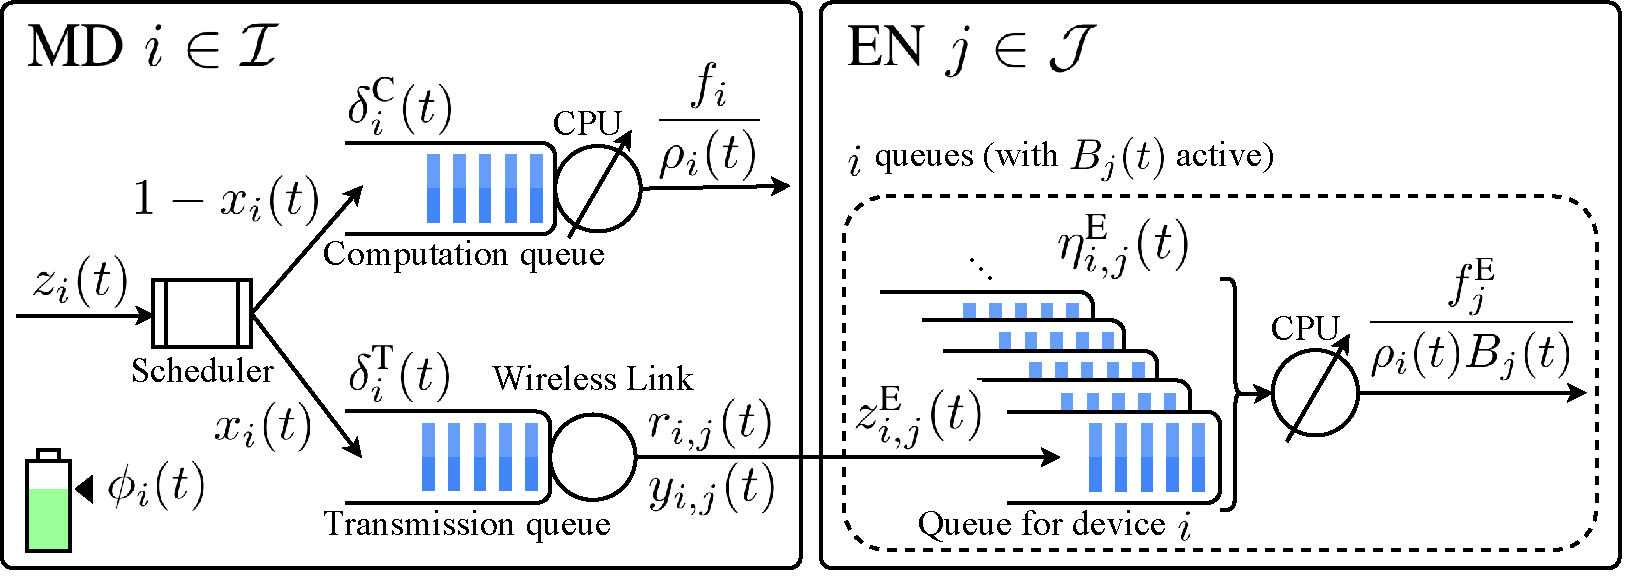
\includegraphics[width=.7\linewidth]{Fig/queue}
	\vspace*{-1mm}
	\caption{An illustration of MD $i \in \mathcal{I}$ and EN $j \in \mathcal{J}$ in the MEC system.}
	\vspace*{-3mm}
	\label{fig1}
\end{figure}

We define $z_i(t)$ as the index assigned to the computation task arriving at MD $i \in \mathcal{I}$ in time slot $t \in \mathcal{T}$. Let $\lambda_i(t)$ denote the size of this task in bits. The size of task $z_i(t)$ is selected from a discrete set $\Lambda = \{\lambda_1, \lambda_2, \ldots, \lambda_{\theta}\}$, where $\theta$ represents the number of these values. Hence, $\lambda_i(t) \in \Lambda \cup \{0\}$ to consider the case that no task has arrived. We also denote the task's processing density as $\rho_i(t)$ that indicates the number of CPU cycles required to complete the execution of a unit of the task. Furthermore, we denote the deadline of this task by $\Delta_i(t)$ which is the number of time slots that the task must be completed to avoid being dropped.
%At the beginning of time slot $t \in \mathcal{T}$, if MD $i \in \mathcal{I}$ has a newly arrived task, we define $z_i(t)$ as the unique index assigned to that task. Let $\lambda_i(t)$ be the number of newly arrived bits at the beginning of time slot $t \in \mathcal{T}$. If a new task $z_i(t)$ exists at the start of time slot $t$, then $\lambda_i(t)$ is equal to the size of task $z_i(t)$. Otherwise, $\lambda_i(t) = 0$. We consider $\rho_i(t)$ to represent the processing density of task $z_i(t)$, indicating the number of CPU cycles required to process a unit of the task.

We define two binary variables, $x_i(t)$ and $y_{i,j}(t)$ for $i \in \mathcal{I}$ and $j \in \mathcal{J}$ to determine the offloading decision and offloading target, respectively. Specifically, $x_i(t)$ indicates whether task $z_i(t)$ is assigned to the computation queue ($x_i(t) = 0$) or to the transmission queue ($x_i(t) = 1$), and $y_{i,j}(t)$ indicates whether task $z_i(t)$ is offloaded to EN $j \in \mathcal{J}$. If the task is dispatched to EN $j$, we set $y_{i,j}(t) = 1$; otherwise, $y_{i,j}(t) = 0$.





\subsection{Communication Model}
We consider that the tasks in the transmission queue are dispatched to the appropriate ENs via the MD wireless interface. We denote the transmission rate of MD $i$'s interface when communicating with EN $j \in \mathcal{J}$ in time $t$ as $r_{i,j}(t)$. In time slot $t \in \mathcal{T}$, if task $z_i(t)$ is assigned to the transmission queue for computation offloading, we define $l_i^{\text{T}}(t) \in \mathcal{T}$ to represent the time slot when the task is either dispatched to the EN or dropped. We also define $\delta_i^{\text{T}}(t)$ as the number of time slots that task $z_i(t)$ should wait in the queue before transmission. It should be noted that MD $i$ computes the value of $\delta_i^{\text{T}}(t)$ before making a decision. The value of $\delta_i^{\text{T}}(t)$ is computed as follows:
\begin{alignat}{1}
	\delta_i^{\text{T}}(t) =\textcolor{white}{i} \left[ \textcolor{white}{i}\max\limits_{t^{'}\textcolor{white}{i} \in \textcolor{white}{i} \{0,1,\ldots,t-1\}} l_i^{\text{T}}\textcolor{white}{i}(t^{'})-t+1\textcolor{white}{i}\right]^+\textcolor{white}{i},
	\label{1}  
\end{alignat}
where $[\cdot]^+ =$ max$(0, \cdot)$ and $l_i^{\text{T}}(0)=0$ for the simplicity of presentation. Note that the value of $\delta_i^{\text{T}}(t)$ only depends on $l_i^{\text{T}}(t)$ for $t' < t$. If MD $i \in \mathcal{I}$ schedules task $z_i(t)$ for dispatching in time slot $t \in \mathcal{T}$, then it will either be dispatched or dropped in time slot $l_i^{\text{T}}(t)$, which is
\begin{alignat}{1}
	l_i^{\text{T}}(t) = \min \Big\{t + \delta_i^{\text{T}}(t) + \lceil{D_i^{\text{T}}(t)}\rceil - 1, t + \Delta_i(t) - 1\Big\},
	\label{2}  
\end{alignat}
where $D_i^{\text{T}}(t)$ refers to the number of time slots required for the transmission of task $z_i(t)$ from MD $i \in \mathcal{I}$ to EN $j \in \mathcal{J}$. We have
\begin{alignat}{1}
	D_i^{\text{T}}(t) =  \sum_{\mathcal{J}} y_{i,j}(t) {\lambda_i(t) \over r_{i,j}(t)\tau}.
	\label{3}  
\end{alignat}
Let $E_i^{\text{T}}(t)$ denote the energy consumption of the transmission from MD $i \in \mathcal{I}$ to EN $j \in \mathcal{J}$. We have
\begin{alignat}{1}
	E_i^{\text{T}}(t) = D_i^{\text{T}}(t)p_i^{\text{T}}(t)\tau,
	\label{4}  
\end{alignat}
where $p_i^{\text{T}}(t)$ represents the power consumption of the communication link of MD $i \in \mathcal{I}$ in time slot $t$.
\subsection{Computation Model}
The computation tasks can be executed either locally on the MD or on the EN. In this subsection, we provide a detailed explanation of these two cases.
\subsubsection{Local Execution}
We model the local execution by a queuing system consisting the computation queue and the MD processor. Let $f_i$ denote the MD $i$'s processing power (in cycle per second). When task $z_i(t)$ is assigned to the computation queue at the beginning of time slot $t \in \mathcal{T}$, we define $l_i^{\text{C}}(t) \in \mathcal{T}$ as the time slot during which task $z_i(t)$ will either be processed or dropped. If the computation queue is empty, $l_i^{\text{C}}(t) = 0$. Let $\delta_i^{\text{C}}(t)$ denote the number of remaining time slots before processing task $z_i(t)$ in the computation queue. We have:
\begin{alignat}{1}
	\delta_i^{\text{C}}(t) = \left[ \max \limits_{t' \in \{0,1,\ldots,t-1\}} l_i^{\text{C}}(t')-t+1 \right]^+.
	\label{5}  
\end{alignat}
%In the above relation, the operator $[z]^+ = \max{0, z}$ is defined, and the variable $l_i^{\text{C}}(0) = 0$. Specifically, the expression $\max_{t' \in {0,1,2,\ldots,t-1}} l_i^{\text{C}}(t')$ determines the time slot until which all tasks placed in the local computation queue have been completed before time slot $t$. Therefore, $\delta_i^{\text{C}}(t)$ represents the number of time slots that task $z_i(t)$ needs to wait for processing. For example, suppose task $z_i(1)$ is in the computation queue, and its processing will be completed in time slot 5. Hence, $l_i^{\text{C}}(1) = 5$, meaning that the task should remain in the queue for $\Delta^{comp}(3) = [\max{5,0}-3+1]^+ = 3$ time slots until the process is finished.
In the equation above, the term $\max_{t' \in \{0, 1, \ldots, t-1\}} l_i^{\text{C}}(t')$ denotes the time slot at which each existing task in the computation queue, which arrived before time slot $t$, is either processed or dropped. Consequently, $\delta_i^{\text{C}}(t)$ denotes the number of time slots that task $z_i(t)$ should wait before being processed. We denote the time slot in which task $z_i(t)$ will be completely processed by $l_i^{\text{C}}(t)$ if it is assigned to the computation queue for local processing in time slot $t$. We have
\begin{alignat}{1}
	l_i^{\text{C}}(t) = \min \Big\{t + \delta_i^{\text{C}}(t) + \lceil D_i^{\text{C}}(t) \rceil - 1, t + \Delta_i(t) - 1\Big\}.
	\label{6}  
\end{alignat}
The task $z_i(t)$ will be immediately dropped if its processing is not completed by the end of the time slot $t + \Delta_i(t) - 1$. In addition, we introduce $D_i^{\text{C}}(t)$ as the number of time slots required to complete the processing of task $z_i(t)$ on MD $i \in \mathcal{I}$. It is given by:
\begin{alignat}{1}
	D_i^{\text{C}}(t) = { \lambda_i(t)  \over  f_i  \tau /  \rho_i(t)}.
	\label{7}  
\end{alignat}



%In particular, the processing of task $z_i(t)$ will commence at time $t + \delta_i^{\text{C}}(t)$. Therefore, the first component of the minimum operator is equal to the duration of time in which task $z_i(t)$ is completed without exceeding its deadline, denoted by $\delta_i^{\text{C}}(t)$. The second component refers to the duration of time in which task $z_i(t)$ becomes expired and discarded. As a result, $l_i^{\text{C}}(t)$ represents the time slot in which task $z_i(t)$ will be completed.
To compute the MD's energy consumption in the time slot $t \in \mathcal{T}$, we define $E_i^{\text{L}}(t)$ as:
\begin{alignat}{1}
	E_i^{\text{L}}(t) =  D_i^{\text{C}}(t) p_i^{\text{C}}  \tau, %=  { \lambda_i(t) \rho_i(t)  \over  f_i} p_i^{\text{C}},
	\label{8}  
\end{alignat}
where $p_i^{\text{C}} = 10^{-27}(f_i)^3$ represents the energy consumption of MD $i$'s CPU frequency \cite{mao2016dynamic}.
\subsubsection{Edge Execution}
We model the edge execution by the queues associated with MDs deployed at ENs. If computation task $z_i(t')$ is dispatched to EN $j$ in time $t' < t$, we let $z_{i,j}^{\text{E}}(t)$ and $\lambda_{i,j}^{\text{E}}(t)$ (in bits) denote the unique index of the task and the size of the task in the $i^{\text{th}}$ queue at EN $j$. We define $\eta_{i,j}^{\text{E}}(t)$ (in bits) as the length of this queue at the end of time slot $t \in \mathcal{T}$. We refer to a queue as an active queue in a certain time slot if it is not empty. That being said, if at least one task is already in the queue from previous time slots or there is a task arriving at the queue, that queue is active. We define $\mathcal{B}_j(t)$ to denote the set of active queues at EN $j$ in time slot $t$.
\begin{alignat}{1}
	\mathcal{B}_j(t) = \textcolor{white}{i}\Big\{i \textcolor{white}{i}\big| i \in \mathcal{I}, \lambda_{i,j}^{\text{E}}(t)>0\,\, \textcolor{white}{i}\text{or}\textcolor{white}{i} \,\, \eta_{i,j}^{\text{E}}(t-1)>0\textcolor{white}{i}\Big\}.\textcolor{white}{i}
	\label{9}  
\end{alignat}
We introduce $b_j(t) \triangleq |\mathcal{B}_j(t)|$ that represents the number of active queues in EN $j \in \mathcal{J}$ in time slot $t \in \mathcal{T}$. In each time slot $t \in \mathcal{T}$, the EN's processing power is divided among its active queues using a generalized processor sharing method~\cite{parekh1993generalized}. Let variable $f_j^{\text{E}}$ (in cycles per second) represent the computational capacity of EN $j$. Therefore, EN $j$ can allocate computational capacity of $f_j^{\text{E}}/(\rho_i(t) b_j(t))$ to each MD $i \in \mathcal{B}_j(t)$ during time slot $t$. To calculate the length of the computation queue for MD $i \in \mathcal{I}$ in EN $j \in \mathcal{J}$, we define $\omega_{i,j}(t)$ (in bits) to represent the number of bits from dropped tasks in that queue at the end of time slot $t \in \mathcal{T}$. The backlog of the queue, referred to as $\eta_{i,j}^{\text{E}}(t)$ is given by:
\begin{alignat}{1}
	\eta_{i,j}^{\text{E}}(t)\hspace{-0.8mm}=\hspace{-1mm}\left[\eta_{i,j}^{\text{E}}(t-1)\hspace{-0.6mm}+\hspace{-0.7mm}\lambda_{i,j}^{\text{E}}(t)\hspace{-0.7mm}-\hspace{-0.7mm}{f_j^{\text{E}}\tau\over \rho_i(t)b_j(t)} -\omega_{i,j}(t)\right]^+\hspace{-1mm}.
	\label{10}  
\end{alignat}
We also define $l_{i,j}^{\text{E}}(t) \in \mathcal{T}$ as the time slot during which the offloaded task $z_{i,j}^{\text{\text{E}}}(t)$ is either processed or dropped by EN $j$. Given the uncertain workload ahead at EN $j$, neither MD $i$ nor EN $j$ has information about $l_{i,j}^{\text{E}}(t)$ until the corresponding task $z_{i,j}^{\text{E}}(t)$ is either processed or dropped. Let $\hat{l}_{i,j}^{\text{E}}(t)$ represent the time slot at which the execution of task $z_{i,j}^{\text{E}}(t)$ starts. In mathematical terms, for $i \in \mathcal{I}$, $j \in \mathcal{J}$, and $t \in \mathcal{T}$, we have:
\begin{alignat}{1}
	\hat{l}_{i,j}^{\text{E}}(t) = \max \{t, \max \limits_{t^{'} \in \{0,1,\ldots,t-1\}} l_{i,j}^{\text{E}}(t^{'})+1\},
	\label{11}  
\end{alignat}
where $l_{i,j}^{\text{E}}(0) = 0$. Indeed, the initial processing time slot of task $z_{i,j}^{\text{E}}(t)$ at EN should not precede the time slot when the task was enqueued or when the previously arrived tasks were processed or dropped. Therefore, $l_{i,j}^{\text{E}}(t)$ is the time slot that satisfies the following constraints. %For $i \in \mathcal{I}$, $j \in \mathcal{J}$, and $t \in \mathcal{T}$,
\begin{alignat}{1}
	\sum_{t^{'}=\hat{l}_{i,j}^{\text{E}}(t)}^{l_{i,j}^{\text{E}}(t)}{f_j^{\text{E}}\tau \over \rho_i(t)b_j(t^{'})}\mathbbm{1}(i \in \mathcal{B}_j(t^{'}))  \geq   \lambda_{i,j}^{\text{E}}(t),
	\label{12}  \\
	\sum_{t^{'}=\hat{l}_{i,j}^{\text{E}}(t)}^{l_{i,j}^{\text{E}}(t)-1}{f_j^{\text{E}}\tau \over \rho_i(t)b_j(t^{'})}\mathbbm{1}(i \in \mathcal{B}_j(t^{'})) < \lambda_{i,j}^{\text{E}}(t),
	\label{13}  
\end{alignat}
where $\mathbbm{1} (z \in \mathbb{Z})$ is the indicator function. In particular, the total processing capacity that EN $j$ allocates to MD $i$ from the time slot $\hat{l}_{i,j}^{\text{E}}(t)$ to the time slot $l_{i,j}^{\text{E}}(t)$ should exceed the size of task $z_{i,j}^{\text{E}}(t)$. Conversely, the total allocated processing capacity from the time slot $l_{i,j}^{\text{E}}(t)$ to the time slot $l_{i,j}^{\text{E}}(t)-1$ should be less than the task's size.

Additionally, we define $D_{i,j}^{\text{E}}(t)$ to represent the quantity of processing time slots allocated to task $z_{i,j}^{\text{E}}(t)$ when executed at EN $j$. This value is given by:
\begin{alignat}{1}
	D_{i,j}^{\text{E}}(t) = { \lambda_{i,j}^{\text{E}}(t) \rho_i(t) \over f_j^{\text{E}} \tau /  b_j(t)}.
	\label{14}  
\end{alignat}
We also define $E_{i,j}^{\text{E}}(t)$ as the energy consumption of processing at EN $j$ in time slot $t$ by MD $i$. This can be calculated as:
\begin{alignat}{1}
	E_{i,j}^{\text{E}}(t) = {D_{i,j}^{\text{E}}(t)  p_j^{\text{E}} \tau \over b_j(t)},  % = { \lambda_{i,j}^{\text{E}}(t) \rho_i(t) \over  f_j^{\text{E}}}p_j^{\text{E}} ,
	\label{15}  
\end{alignat}
where $p_j^{\text{E}}$ is a constant value which denotes the energy consumption of the EN $j$'s processor when operating at full capacity. 

In addition to the energy consumed by EN $j$ for task processing, we also take into account the energy consumed by the MD $i$'s user interface in the standby state while waiting for task completion at the EN $j$. We define $E_{i,j}^{\text{I}}(t)$ as the energy consumption associated with the user interface of MD $i \in \mathcal{I}$, which is given by
\begin{alignat}{1}
	E_i^{\text{I}}(t) = D_{i,j}^{\text{E}}(t) p_i^{\text{I}} \tau, %= {\lambda_{i,j}^{\text{E}}(t) \rho_i(t) \over \mathcal{B}_j(t) f_j^{\text{E}}} p_i^{\text{I}},
	\label{16}
\end{alignat}
where $p_i^{\text{I}}$ is the standby energy consumption of MD $i \in \mathcal{I}$.
\begin{alignat}{1}
	E_i^{\text{O}}(t) = E_i^{\text{T}}(t) + \sum_{\mathcal{J}} E_{i,j}^{\text{E}}(t) + E_i^{\text{I}}(t).
	\label{17}
\end{alignat}



\section{Task Offloading problem Formulation}
\label{section:III}

Based on the introduced system model, we present the computation task offloading problem in this section. Our primary goal is to enhance each MD's QoE individually by taking the dynamic demands of MDs into account. To achieve this, we approach the optimization problem as an MDP, aiming to maximize the MD's QoE by striking a balance among key QoE factors, including task completion, task delay, and energy consumption. To prioritize QoE factors, we utilize the MD's battery level, which plays a crucial role in decision-making. Specifically, when an MD observes its state (e.g. task size, queue details, and battery level) and encounters a newly arrived task, it selects an appropriate action for that task. The selected action, based on the observed state, will result in enhanced QoE. Each MD strives to maximize its long-term QoE by optimizing the policy mapping from states to actions. In what follows, we first present the state space, action space, and QoE function, respectively. We then formulate the QoE maximization problem for each MD.




\subsection{State Space}
A state in our MDP represents a conceptual space that comprehensively describes the state of an MD facing the environment. We represent the MD $i$'s state in time slot $t$ as vector $\boldsymbol{s}_i(t)$ that includes the newly arrived task size, the queues information, the MD's battery level, and the workload history at the ENs. The MD observers this vector at the beginning of each time slot. The vector $\boldsymbol{s}_i(t)$ is defined as follows:
\begin{alignat}{1}
	\boldsymbol{s}_i(t) = \Big(\lambda_i(t), \delta_i^{\text{C}}(t), \delta_i^{\text{T}}(t), \boldsymbol{\eta}_i^{\text{E}}\hspace{-0.4mm}(\hspace{-0.4mm}t\hspace{-0.4mm}-\hspace{-0.4mm}1\hspace{-0.5mm}),\phi_i(t), \mathcal{H}(t) \Big),
	\label{18}
\end{alignat}
where vector $\boldsymbol{\eta}_i^{\text{E}}(t-1) = (\eta_{i,j}^{\text{E}}(t-1))_{j \in \mathcal{J}}$ represents the queues length of MD $i$ in ENs at the previous time slot and is computed by the MD according to \eqref{10}. Let $\phi_i(t)$ denote the battery level of MD $i$ in time slot $t$. Considering the power modes of a real mobile device, $\phi_i(t)$ is derived from the discrete set $\Phi=\{\phi_1,\phi_2,\phi_3\}$, corresponding to ultra power-saving, power-saving, and performance modes, respectively.

In addition, to predict future EN workloads, we define the matrix $\mathcal{H}(t)$ as historical data, indicating the number of active queues for all ENs. This data is recorded over $T^{\text{s}}$ time slots, ranging from $t\hspace{-0.4mm}-\hspace{-0.4mm}T^{\text{s}}$ to $t\hspace{-0.4mm}-\hspace{-0.4mm}1$, in $T^{\text{s}}\hspace{-0.4mm}\times \hspace{-0.4mm} J$ matrix. For EN $j$ workload history at $i^{th}$ time slot from $T^{\text{s}}-t$, we define $h_{i,j}(t)$ as:
\begin{alignat}{1}
	h_{i,j}(t) = b_j(t - T^{\text{s}} + i - 1).
	\label{19}
\end{alignat}
%where $b_j(t - T^{\text{s}} + i - 1)$ is the number of active queues of EN $j$ in time slot $t - T^{\text{s}} + i - 1$. 
EN $j \in \mathcal{J}$ broadcasts $b_j(t)$ at the end of each time slot. %Given $b_j(t) \leq I$, can be represented using only a few bits, the broadcast incurs minimal signaling overhead.

We define vector $\mathcal{S}$ as the discrete and finite state space for each MD. The size of the set $\mathcal{S}$ is given by $\Lambda \times T^2 \times \mathcal{U} \times 3 \times I^{T^{\text{s}} \times J}$, where $\mathcal{U}$ is the set of available queue length values at an EN over $T$ time slots. 



%A MD $i \in \mathcal{I}$ can obtain state information $\lambda_i(t)$, $\delta_i^{\text{C}}(t)$, $\delta_i^{\text{T}}(t)$, and $\phi_i(t)$ through local observation at the beginning of time slot $t$.


%For state information  $\boldsymbol{\eta}_i^{\text{E}}(t-1)$, MD $i$ can compute this vector according to the number of transmitted bits to each EN in each time slot and the number of bits of MD $i$ processed or being dropped by each EN in each time slot according to \eqref{10}. 


%For matrix $\mathcal{H}(t)$, we assume that each EN will broadcast its number of active queues at the end of each time slot. Since the number of active queues is always a small number, which can be represented by several bits, the broadcasting will only incur a small signaling overhead.

\subsection{Action Space}
The action space represents the agent's behavior and the decisions. In this context, we define $\boldsymbol{a}_i(t)$ to denote the action taken by MD $i \in \mathcal{I}$ in time slot $t \in \mathcal{T}$. These actions involve two decisions, (a) Offloading decision to determine whether or not to offload the task, and (b) Offloading target to determine the EN to send the offloaded tasks. Thus, the action of MD $i$ in time slot $t$ can be concisely expressed as the following action tuple: \vspace{-1.5mm}
\begin{alignat}{1}
	\boldsymbol{a}_i(t) = (x_i(t), \boldsymbol{y}_i(t)),
	\label{20}
\end{alignat}
where vector $\boldsymbol{y}_i(t)=(y_{i,j}(t))_{j \in \mathcal{J}}$ represents the selected EN for offloading this task. In Section~\ref{section:1}, we will discuss about the size of this action space.

%Hence, the decision space of each MD is thus equal to $\mathcal{A} = \{0,1\}^{1+N}$, with $j$ representing the number of available ENs.



\subsection{QoE Function}
The QoE function evaluates the influence of agent's actions by taking several key performance factors into account. Given the selected action $\boldsymbol{a}_i(t)$ in the observed state $\boldsymbol{s}_i(t)$, we represent $\mathcal{D}_i(\boldsymbol{s}_i(t), \boldsymbol{a}_i(t))$ as the delay of task $z_i(t),$ which indicates the number of time slots from time slot $t$ to the time slot in which task $z_i(t)$ is processed. It is calculated by: 

$\mathcal{D}_i(\boldsymbol{s}_i(t),\boldsymbol{a}_i(t)) = (1-x_i(t))\Big(l_i^{\text{C}}(t) - t + 1\Big)  +$
\begin{alignat}{1}
	\;\;\;\; x_i(t)\bigg( \sum\limits_{\mathcal{J}} \sum\limits_{t'=t}^{T}\mathbbm{1}\big(z_{i,j}^{\text{E}}(t')=z_i(t)\big) l_{i,j}^{\text{E}}(t') - t +1\bigg),
	\label{21}  
\end{alignat} 
where $\mathcal{D}_i(\boldsymbol{s}_i(t),\boldsymbol{a}_i(t))= 0$ when task $z_i(t)$ is dropped. Correspondingly, we denote the energy consumption of task $z_i(t)$ when taking action $\boldsymbol{a}_i(t)$ in the observed state $\boldsymbol{s}_i(t)$ as $\mathcal{E}_i(\boldsymbol{s}_i(t),\boldsymbol{a}_i(t))$, which is: \vspace{1.7mm}

$\mathcal{E}_i(\boldsymbol{s}_i(t),\boldsymbol{a}_i(t)) = (1-x_i(t)) E_i^{\text{L}}(t)+$
\begin{alignat}{1}
	\hspace{1.8cm} x_i(t)\bigg( \sum\limits_{\mathcal{J}} \sum\limits_{t^{'}=t}^{T}\mathbbm{1}\big(z_{i,j}^{\text{E}}(t') = z_i(t)\big) E_i^{\text{O}}(t)  \bigg).
	\label{22}  
\end{alignat}
Given the delay and energy consumtion of task $z_i(t)$, we also define $\mathcal{C}_i(\boldsymbol{s}_i(t),\boldsymbol{a}_i(t))$ that denotes the assosiate cost of task $z_i(t)$ given the action $\boldsymbol{a}_i(t)$ in the state $\boldsymbol{s}_i(t)$. \vspace{1.7mm}


$\mathcal{C}_i(\boldsymbol{s}_i(t),\boldsymbol{a}_i(t)) =$
\begin{alignat}{1}
	\phi_i(t) \, \mathcal{D}_i(\boldsymbol{s}_i(t),\boldsymbol{a}_i(t)) +(1-\phi_i(t)) \, \mathcal{E}_i(\boldsymbol{s}_i(t),\boldsymbol{a}_i(t)),
	\label{23}  
\end{alignat}
where $\phi_i(t)$ represents the MD $i$'s battery level. When the MD is operating in performance mode, the primary focus is on minimizing task delays, thus the delay contributes more to the cost. On the other hand, when the MD switches to ultra power-saving mode, the main attention is directed toward reducing power consumption.

Finally, we define $\boldsymbol{q}_i(\boldsymbol{s}_i(t),\boldsymbol{a}_i(t))$ as the QoE associated with task $z_i(t)$ given the selected action $\boldsymbol{a}_i(t)$ and the observed state $\boldsymbol{s}_i(t)$. The QoE function is defined as follows:\vspace{1.7mm}

$\boldsymbol{q}_i(\boldsymbol{s}_i(t),\boldsymbol{a}_i(t)) =$
\begin{alignat}{1}
	\hspace*{8mm}
	\begin{cases} 
		\mathcal{R} - \mathcal{C}_i(\boldsymbol{s}_i(t),\boldsymbol{a}_i(t)) & \hspace*{-2mm} \text{if task $z_i(t)$ is processed,} \\
		- \hspace*{0.8mm} \mathcal{E}_i(\boldsymbol{s}_i(t),\boldsymbol{a}_i(t)) &	\hspace*{-2mm} \text{if task $z_i(t)$ is dropped,}
	\end{cases}
	\label{26}  
\end{alignat}
where $\mathcal{R} > 0$ represents a constant reward for task completion. If $z_i(t) = 0$, then $\boldsymbol{q}_i(\boldsymbol{s}_i(t), \boldsymbol{a}_i(t)) = 0$. Throughout the rest of this paper, we adopt the shortened notation $\boldsymbol{q}_i(t)$ to represent $\boldsymbol{q}_i(\boldsymbol{s}_i(t), \boldsymbol{a}_i(t))$.
%When $\phi_i(t)$ is closer to 1, the cost function prioritizes reducing delay and drop, which could be advantageous in situations where tasks need to be completed quickly, and responsiveness is crucial. Conversely, when $\phi_i(t)$ is closer to 0, the cost function prioritizes reducing energy consumption, which is beneficial when the MD's battery level is low, and conserving power is necessary to prolong operation.

\subsection{Problem Formulation}
We define the task offloading policy for MD $i \in \mathcal{I}$ as a mapping from its state to its corresponding action, denoted by i.e., $\pi_i : \mathcal{S} \rightarrow \mathcal{A}$. Especially, MD $i$ determines an action $\boldsymbol{a}_i(t) \in \mathcal{A}$, according to policy $\pi_i$ given the observed environment state $\boldsymbol{s}_i(t) \in \mathcal{S}$. The MD aims to find its optimal policy $\pi_i^*$ which maximizes the long-term QoE,
\begin{alignat}{1}
	\pi_i^* = \text{arg}\,\,  \max\limits_{\pi_i}  \mathbbm{E} \Bigg[ \sum\limits_{t \in \mathcal{T}}  \gamma^{t-1}\boldsymbol{q}_i(t) \Bigg| \pi_i \Bigg],
	\label{24}  
\end{alignat}
where $\gamma \in (0,1]$ is a discount factor and determines the balance between instant QoE and long-term QoE. As $\gamma$ approaches 0, the MD prioritizes QoE within the current time slot exclusively. Conversely, as $\gamma$ approaches 1, the MD increasingly factors in the cumulative long-term QoE. The expectation $\mathbb{E}[\cdot]$ is taken into consideration of the time-varying system environments. Solving the optimization problem in \eqref{24} is particularly challenging due to the dynamic nature of the network. To address this challenge, we introduce a DRL- based offloading algorithm to learn the mapping between each state-action pair and their long-term QoE.
\section{DRL-Based Offloading Algorithm} \label{section:IV}
We now present QECO algorithm so as to address the distributed offloading decision-making of MDs. The aim is to empower MDs to identify the most efficient action that maximizes their long-term QoE. In the following, we introduce a neural network that characterizes the MD's state-action Q-values mapping, followed by a description of the information exchange between the MDs and ENs.

\begin{figure}
	\centering
	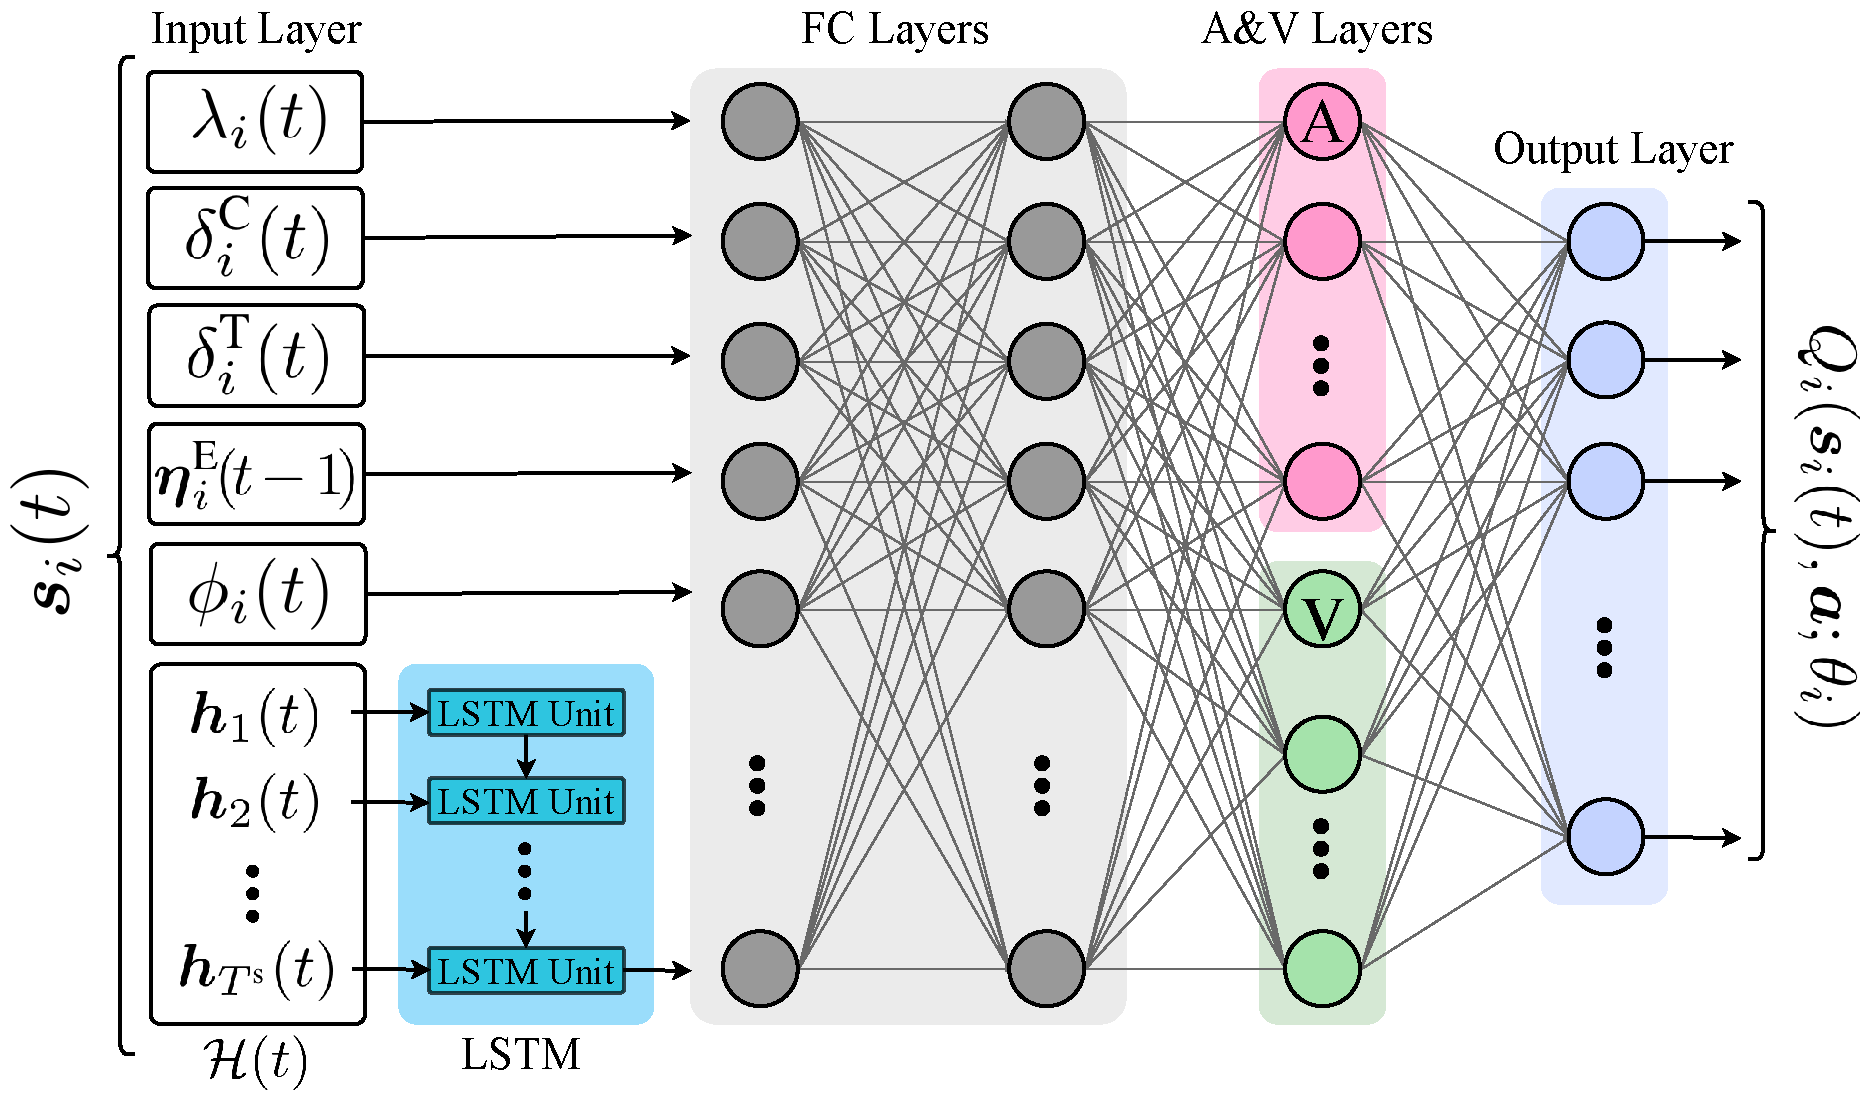
\includegraphics[width=0.7\linewidth]{Fig/DQN}
	\captionsetup{name=Fig.}
	
	\caption{The neural network of MD $i \in \mathcal{I}$, which characterize the Q-value of each action $\boldsymbol{a} \in \mathcal{A}$ under state $\boldsymbol{s}_i(t) \in \mathcal{S}$.}
	\vspace*{-4.5mm}
	\label{DQN}
\end{figure}


\subsection{DQN-based Approach}
We utilize the DQN technique to find the mapping between each state-action pair to Q-values in the formulated MDP. As shown in Fig.~\ref{DQN}, each MD $i \in \mathcal{I}$ is equipped with a neural network comprising six layers. These layers include an input layer, an LSTM layer, two dense layers, an advantage-value (A\&V) layer, and an output layer. The parameter vector $\theta_i$ of MD $i$'s neural network is defined to maintain the connection weights and neuron biases across all layers. For MD $i \in \mathcal{I}$, we utilize the state information as the input of neural network. The state information $\lambda_i(t)$, $\delta_i^{\text{C}}(t)$, $\delta_i^{\text{T}}(t)$, $\phi_i(t)$, and $\boldsymbol{\eta}_i^{\text{E}}(t-1)$ are directly passed to the dense layer, while the state information $\mathcal{H}(t)$ is first supplied to the LSTM layer and then the resulting output is sent to the dense layer. The role and responsibilities of each layer are detailed as follows.


\subsubsection{Predicting Workloads at ENs}
In order to capture the dynamic behavior of workloads at the ENs, we employ the LSTM network \cite{hochreiter1997long}. This network maintains a memory state $\mathcal{H}(t)$ that evolves over time, enabling the neural network to predict future workloads at the ENs based on historical data. By taking the matrix $\mathcal{H}(t)$ as an input, the LSTM network learns the patterns of workload dynamics. The architecture of the LSTM consists of $T^{\text{s}}$ units, each equipped with a set of hidden neurons, and it processes individual rows of the matrix $\mathcal{H}(t)$ sequentially. Through this interconnected design, MD tracks the variations in sequences from $\boldsymbol{h}_1(t)$ to $\boldsymbol{h}_{T^{\text{s}}}(t)$, where vector $\boldsymbol{h}_i(t) = (h_{i,j}(t))_{j \in \mathcal{J}}$, thereby revealing workload fluctuations at the ENs across different time slots. The final LSTM unit produces an output that encapsulates the anticipated workload dynamics, and is then connected to the subsequent layer neurons for further learning.




%\subsubsection{workload Prediction}
%To learning the dynamics of the workloads at the ENs, we use the LSTM network [26], [27], which can keep track of the state $\mathcal{H}(t)$ over time. It can provide the neural network the ability of estimating the workloads at the ENs in the future using the history. The LSTM network takes the matrix $\mathcal{H}(t)$ as input so as to learn the workload dynamics. coresponding the matrix $\mathcal{H}(t)$,  The LSTM network contains $T^{\text{s}}$ LSTM units, each of which contains a set of hidden neurons and takes one row of the matrix $\mathcal{H}(t)$ as input. These LSTM units are connected in sequence so as to keep track of the variations of the sequences from $\{\mathcal{H}(t)\}_1$ to $\{\mathcal{H}(t)\}_{T^{\text{s}}}$, which can reveal the variations of the workloads at the ENs among time slots. The LSTM network will output the information that indicates the dynamics of the workloads in the future in the last LSTM unit, where the output will be connected to the neurons in the next layer for further learning.
%
%---------------------

%This layer is responsible for learning the dynamics of the workloads at the ENs. This is achieved by including an LSTM network [26], [27]. We use the LSTM network because it can keep track of the state $\textbf{H}(t)$ over time. It can provide the neural network the ability of estimating the workloads at the ENs in the future using the history. 
%
%Specifically, the LSTM network takes the matrix $\textbf{H}(t)$ as input so as to learn the workload dynamics. Fig. 3 shows the structure of an LSTM network. The LSTM network contains Tstep LSTM units, each of which contains a set of hidden neurons. Each LSTM unit takes one row of the matrix $\textbf{H}(t)$ as input, we let $\{\textbf{H}(t)\}_1$  denote the $i^{th}$ row of matrix $\textbf{H}(t)$ in Fig. 3. These LSTM units are connected in sequence so as to keep track of the variations of the sequences from $\{\textbf{H}(t)\}_1$ to $\{\textbf{H}(t)\}_{T^{step}}$, which can reveal the variations of the workloads at the ENs among time slots. The LSTM network will output the information that indicates the dynamics of the workloads in the future in the last LSTM unit, where the output will be connected to the neurons in the next layer for further learning.



\subsubsection{State-Action Q-Value Mapping}
The pair of dual dense layers plays a crucial role in learning the mapping of Q-values from the current state and the learned load dynamics to the corresponding actions. The dense layers consist of a cluster of neurons that employ rectified linear units (ReLUs) as their activation functions. In the initial dense layer, connections are established from the neurons in the input layer and the LSTM layer to each neuron in the dense layer. The resulting output of a neuron in the dense layer is connected to each neuron in the subsequent dense layer. In the second layer, the outputs from each neuron establish connections with all neurons in the A\&V layers.



\subsubsection{Dueling-DQN Approach for Q-Value Estimation}
In the neural network architecture, the A\&V layer and the output layer incorporate the principles of the dueling-DQN \cite{wang2016dueling} to compute action Q-values. The fundamental concept of dueling-DQN involves two separate learning components: one for action-advantage values and another for state-value. This approach enhances Q-value estimation by separately evaluating the long-term QoE attributed to states and actions.



The A\&V layer consists of two distinct dense networks referred to as network A and network V. Network A's role is to learn the action-advantage value for each action, while network V focuses on learning the state-value. For an MD $i \in \mathcal{I}$, we define $V_i(\boldsymbol{s}_i(t); \theta_i)$ and $A_i(\boldsymbol{s}_i(t), \boldsymbol{a}; \theta_i)$ to denote the state-value and the action-advantage value of action $\boldsymbol{a} \in \mathcal{A}$ under state $\boldsymbol{s}_i(t) \in \mathcal{S}$, respectively. The parameter $\theta_i$ is responsible for determining these values, and it can be adjusted when training the QECO algorithm.

For an MD $i \in \mathcal{I}$, the A\&V layer and the output layer collectively determine $Q_i(\boldsymbol{s}_i(t), \boldsymbol{a}; \theta_i)$, representing the resulting Q-value under action $\boldsymbol{a} \in \mathcal{A}$ and state $\boldsymbol{s}_i(t) \in \mathcal{S}$, as follows: \vspace{1.7mm}


$Q_i(\boldsymbol{s}_i(t), \boldsymbol{a}; \theta_i) = V_i(\boldsymbol{s}_i(t);\theta_i) +$
\begin{alignat}{1}
	\hspace{0.94cm} \Bigg( A_i(\boldsymbol{s}_i(t),\boldsymbol{a};\theta_i) - {1 \over |\mathcal{A}|} \sum\limits_{\boldsymbol{a}' \in \mathcal{A}}(A_i(\boldsymbol{s}_i(t),\boldsymbol{a}';\theta_i) \Bigg),
	\label{25}  
\end{alignat}
where $\theta_i$ establishes a functional relationship that maps Q-values to pairs of state-action.

%, which characterizes the long-term QoE under any observed state $\boldsymbol{s}_i(t) \in \mathcal{S}$ and action $\mathcal{A} \in \mathcal{A}$. 


%\begin{algorithm} [tbp]
%	\caption{QECO Algorithm (Offloading Decision)}\label{alg:cap}
%	\begin{algorithmic}[1]
	%		\renewcommand{\algorithmicrequire}{\textbf{Input:}} 
	%		\renewcommand{\algorithmicensure}{\textbf{Output:}}
	%		\Require state space $\mathcal{S}$, action space $\mathcal{A}$
	%		\Ensure MD $i \in \mathcal{I}$ experience 
	%		\For {episode 1 to $N^{\text{ep}}$}
	%		\State Initialize $\boldsymbol{s}_i(1)$
	%		\For {time slot $t \in \mathcal{T}$}
	%		\If{MD $i$ receives a new task $z_i(t)$}
	%		\State Send an \textit{UpdateRequest} to EN $j_i$;
	%		\State Receive network parameter vector $\theta_i^{\text{E}}$;
	%		\State Select action $\boldsymbol{a}_i(t)$ based on \eqref{26};
	%		\EndIf
	%		\State Observe a set of QoEs $\{\boldsymbol{q}_i(t'), t' \in \mathcal{F}_i^t\}$;
	%		\State Observe\textcolor{white}{i}the next\textcolor{white}{i}state $\textbf{\textit{s}}_i(t+1)$;\textcolor{white}{i}
	%		\For {each task $z_i(t')$ where $t' \in \mathcal{F}_i^t$} 
	%		\State Send \hspace{-1mm} $(\boldsymbol{s}_i(t'), \boldsymbol{a}_i(t'), \boldsymbol{q}_i(t'), \boldsymbol{s}_i(t'\hspace{-1mm}+1))$ to EN $j_i$;
	%		\EndFor
	%		\EndFor
	%		\EndFor
	%	\end{algorithmic}
%\end{algorithm}


\subsection{QoE-Oriented DRL-Based Algorithm}
\label{section:1}

%Our proposed QoE-Driven DRL-Based Algorithm is designed to efficiently distribute computational loads for training neural networks on MDs while leveraging the support of ENs. The primary objective of this algorithm is to utilize the experience of each MD to train its neural network, allowing the MD to make informed decisions that maximize its long-term QoE. To achieve efficient training, each MD $i \in \mathcal{I}$ is paired with a dedicated EN $n_i \in \mathcal{J}$ that assists in the training process. The selection of EN $n_i$ is based on its maximum transmission capacity with MD $i$. We define the set $\mathcal{I}_j \subset \mathcal{I}$ as the group of MDs whose training is facilitated by EN $j \in \mathcal{J}$.

The QECO algorithm is meticulously designed to optimize the allocation of computational tasks between MDs and ENs. Since the training of neural networks imposes an extensive computational workload on MDs, we enable MDs to utilize ENs for training their neural networks, effectively reducing their computational workload. For each MD $i \in \mathcal{I}$, there is an associated EN, denoted as EN $j_i \in \mathcal{J}$, which assists in the training process. This EN possesses the highest transmission capacity among all ENs. We define $\mathcal{I}_j \subset \mathcal{I}$ as the set of MDs for which training is executed by EN $j \in \mathcal{J}$, i.e. $\mathcal{I}_j = \{i \in \mathcal{I} | j_i = j\}$. This approach is feasible due to the minimal information exchange and processing requirements for training compared to MD's tasks. The algorithms to be executed at MD $i \in \mathcal{I}$ and EN $j \in \mathcal{J}$ are given in Algorithms ~\ref{alg:cap} and ~\ref{alg:cap2}, respectively. The core concept involves training neural networks with MD experiences (i.e., state, action, QoE, next state) to map Q-values to each state-action pair. This mapping allows MD to identify the action in the observed state with the highest Q-value and maximize its long-term QoE.




In detail, EN $j \in \mathcal{J}$ maintains a replay buffer denotes as $\mathcal{M}_i$ with two neural networks for MD $i$: $\textit{Net}_i^{\text{E}}$, denoting the evaluation network, and $\textit{Net}_i^{\text{T}}$, denoting the target network, which have the same neural network architecture. However, they possess distinct parameter vectors $\theta^{\text{E}}_i$ and $\theta^{\text{T}}_i$, respectively. Their Q-values are represented by $Q_i^{\text{E}}(\boldsymbol{s}_i(t), \boldsymbol{a}; \theta^{\text{E}}_i)$ and $Q_i^{\text{T}}(\boldsymbol{s}_i(t), \boldsymbol{a}; \theta^{\text{T}}_i)$ for MD $i \in \mathcal{I}_j$, respectively, associating the action $\boldsymbol{a} \in \mathcal{A}$ under the state $\boldsymbol{s}_i(t) \in \mathcal{S}$. The replay buffer records the observed experience $(\boldsymbol{s}_i(t), \boldsymbol{a}_i(t), \boldsymbol{q}_i(t), \boldsymbol{s}_i(t+1))$ of MD $i$. Moreover, $\textit{Net}_i^{\text{E}}$ is responsible for action selection, while $\textit{Net}_i^{\text{T}}$ characterizes the target Q-values, which represent the estimated long-term QoE resulting from an action in the observed state. The target Q-value serves as the reference for updating the network parameter vector $\theta^{\text{E}}_i$. This update occurs through the minimization of disparities between the Q-values under $\textit{Net}_i^{\text{E}}$ and $\textit{Net}_i^{\text{T}}$. In the following, we introduce the offloading decision algorithm of MD $i \in \mathcal{I}$ and the training process algorithm running in EN $j \in \mathcal{J}$.

% i.e., $\textbf{\textit{s}}_i(1) = \big(\lambda_i(1), \delta_i^{\text{C}}(1), \delta_i^{\text{T}}(1), \boldsymbol{\eta}_i^{\text{E}}(0),\phi_i(1), \mathcal{H}(1) \big)$, where we set $\boldsymbol{\eta}_i^{\text{E}}(0)=0$ for all $j \in \mathcal{J}$, and $ \mathcal{H}(1)$ is a zero matrix with size $T^s \times N$. 




\subsubsection{Offloading Decision Algorithm at MD $i \in \mathcal{I}$}
We analyze a series of episodes, where $N^{\text{ep}}$ denotes the number of them. At the beginning of each episode, if MD $i \in \mathcal{I}$ receives a new task $z_i(t)$, it initializes the state $\mathcal{S}_i(1)$ and sends an $\textit{UpdateRequest}$ to EN $j_i$. After receiving the requested vector $\theta_i^{\text{E}}$ of $\textit{Net}_i^{\text{E}}$ from EN $j_i$, MD $i$ chooses the following action for task $z_i(t)$.
\begin{alignat}{1}
	\hspace*{-2mm}\boldsymbol{a}_i(t) \hspace*{-0.5mm} = \hspace*{-0.5mm}
	\begin{cases} 
		\text{arg $\max_{\boldsymbol{a}\in \mathcal{A}}Q_i^{\text{E}}(\boldsymbol{s}_i(t), \boldsymbol{a}; \theta^{\text{E}}_i)$,} & \text{w.p. $1-\boldsymbol{\epsilon}$,} \\
		\text{pick a random action from $\mathcal{A}$,} & \text{w.p. $\boldsymbol{\epsilon}$,}
	\end{cases}
	\label{26}  
\end{alignat}
where w.p. stands for with probability, and $\boldsymbol{\epsilon}$ represents the random exploration probability. The value of $Q_i^{\text{E}}(\boldsymbol{s}_i(t), \boldsymbol{a}; \theta^{\text{E}}_i)$ indicates the Q-value under the parameter $\theta^{\text{E}}_i$ of the neural network $\textit{Net}_i^{\text{E}}$. Specifically, the MD with a probability of $1 - \boldsymbol{\epsilon}$ selects the action associated with the highest Q-value under $\textit{Net}_i^{\text{E}}$ in the observed state $\boldsymbol{s}_i(t)$.


In the next time slot $t+1$, MD $i$ observes the state $\mathcal{S}_i(t+1)$. However, due to the potential for tasks to extend across multiple time slots, QoE $\boldsymbol{q}_i(t)$ associated with task $z_i(t)$ may not be observable in time slot $t+1$. On the other hand, MD $i$ may observe a group of QoEs associated with some tasks $z_i(t')$ in time slots $t' \leq t$. For each MD $i$, we define the set $\mathcal{F}_i^t \subset \mathcal{T}$ to denote the time slots during which each arriving task $z_i(t')$ is either processed or dropped in time slot $t$, as given by: \vspace{2mm}

$\mathcal{F}_i^t =\bigg \{ t' \bigg|\; t' \leq t,\; \lambda_i(t')>0, \; (1 - x_i(t')) \; l_i^{\text{C}}(t') \; + $ \vspace{-3mm}
\begin{equation}
	\hspace{20mm} x_i(t')\sum\limits_{\mathcal{J}} \sum\limits_{n= t'}^{t}\mathbbm{1}(z_{i,j}^{\text{E}}(n)=z_i(t'))  \; l_{i,j}^{\text{E}}(n) = t \bigg\}.
	\label{27}  
	\nonumber
\end{equation}
Therefore, MD $i$ observes a set of QoEs $\{\boldsymbol{q}_i(t') \mid t' \in \mathcal{F}_i^t\}$ at the beginning of time slot $t+1$, where the set $\mathcal{F}_i^t$ for some $i \in \mathcal{I}$ can be empty. Subsequently, MD $i$ sends its experience $(\boldsymbol{s}_i(t), \boldsymbol{a}_i(t), \boldsymbol{q}_i(t), \boldsymbol{s}_i(t+1))$ to EN $j_i$ for each task $z_i(t')$ in $t' \in \mathcal{F}_i^t$.


%\begin{algorithm}[tbp]
%	\caption{QECO Algorithm (Training Process)}\label{alg:cap2}
%	\begin{algorithmic}[1]
	%		\State Initialize replay buffer $\mathcal{M}_i$ for each MD $i \in \mathcal{I}_j$;
	%		\State Initialize $\textit{Net}_i^{\text{E}}$ and $\textit{Net}_i^{\text{T}}$ with random parameters $\theta_i^{\text{E}}$ and $\theta_i^{\text{T}}$ respectively, for each MD $i \in \mathcal{I}_j$;
	%		\State Set Count := 0
	%		\While{True} \Comment{\textit{infinite loop}}
	%		\If{receive an \textit{UpdateRequest} from MD $i \in \mathcal{I}_j$}
	%		\State Send  $\theta_i^{\text{E}}$ to MD $i \in \mathcal{I}$;
	%		\EndIf
	%		\If {an experience \hspace{-0.2mm} $(\hspace{-0.2mm}\boldsymbol{s}_i(\hspace{-0.2mm}t\hspace{-0.2mm}), \boldsymbol{a}_i(\hspace{-0.2mm}t\hspace{-0.2mm}), \boldsymbol{q}_i(\hspace{-0.2mm}t\hspace{-0.2mm}), \boldsymbol{s}_i(\hspace{-0.2mm}t\hspace{-0.3mm}+\hspace{-0.3mm}\hspace{-0.2mm}1\hspace{-0.2mm}\hspace{-0.2mm})\hspace{-0.2mm})$ is received \\ \;\;\;\; from MD $i \in \mathcal{I}_j$}
	%		\State Store $(\boldsymbol{s}_i(t'), \boldsymbol{a}_i(t'), \boldsymbol{q}_i(t'), \boldsymbol{s}_i(t'\hspace{-1mm}+1))$ in $\mathcal{M}_i$;
	%		\State Get a collection of experiences  $\mathcal{I}$ from $\mathcal{M}_i$; 
	%		\For{each experience $i \in \mathcal{I}$} 
	%		\State Get experience $(\boldsymbol{s}_i(\hspace{-0.2mm}n\hspace{-0.2mm}), \boldsymbol{a}_i(\hspace{-0.2mm}n\hspace{-0.2mm}), \boldsymbol{q}_i(\hspace{-0.2mm}n\hspace{-0.2mm}), \boldsymbol{s}_i(\hspace{-0.2mm}n\hspace{-0.5mm}+1\hspace{-0.2mm}))$; 
	%		\State Generate $\hat{Q}_{i,n}^{\text{T}}$ according to   \eqref{28};
	%		\EndFor
	%		\State Set vector  $\hat{\mathbf{Q}}_i^{\text{T}} := (\hat{Q}^{\text{T}}_{i,n})_{n \in \mathcal{N}}$;
	%		\State Update $\theta_i^{\text{E}}$ to minimize $L(\theta_i^{\text{E}}$, $\hat{\mathbf{Q}}_i^{\text{T}})$ in   \eqref{30};
	%		\State Count := Count + 1;
	%		\If {mod(Count, \textit{ReplaceThreshold}) = 0}
	%		\State $\theta_i^{\text{T}}$ := $\theta_i^{\text{E}}$;
	%		\EndIf
	%		\EndIf
	%		\EndWhile
	%		
	%	\end{algorithmic}
%\end{algorithm}


\subsubsection{Training Process Algorithm at EN $j \in \mathcal{J}$}
Upon initializing the replay buffer $\mathcal{M}_i$ with the neural networks $\textit{Net}_i^{\text{E}}$ and $\textit{Net}_i^{\text{T}}$ for each MD $i \in \mathcal{I}_j$, EN $j \in \mathcal{J}$ waits for messages from the MDs in the set $\mathcal{I}_j$. When EN $j$ receives an $\textit{UpdateRequest}$ signal from an MD $i \in \mathcal{I}_j$, it responds by transmitting the updated parameter vector $\theta^{\text{E}}_i$, obtained from $\textit{Net}_i^{\text{E}}$, back to MD $i$. On the other side, if EN $j$ receives an experience $(\boldsymbol{s}_i(t), \boldsymbol{a}_i(t), \boldsymbol{q}_i(t), \boldsymbol{s}_i(t+1))$ from MD $i \in \mathcal{I}_j$, the EN stores this experience in the replay buffer $\mathcal{M}_i$ associated with that MD. %The replay buffer operates at maximum capacity and FIFO principle.

The EN randomly selects a sample collection of experiences from the replay buffer, denoted as $\mathcal{N}$. For each experience $n \in \mathcal{N}$, it calculates the value of $	\hat{Q}^{\text{T}}_{i,n}$. This value represents the QoE in experience $n$ and includes a discounted Q-value of the action anticipated to be taken in the subsequent state of experience $n$, according to the network $\textit{Net}^\text{T}_i$, given by
\begin{alignat}{1}
	\hat{Q}_{i,n}^{\text{T}} = \boldsymbol{q}_i(n) + \gamma Q_i^{\text{T}}(\boldsymbol{s}_i(n+1)), \tilde{\boldsymbol{a}}_n; \theta_i^{\text{T}}),
	\label{28}  
\end{alignat}  
where $\tilde{\boldsymbol{a}}_n$ denotes the optimal action for the state $\boldsymbol{s}_i(n+1)$ based on its highest Q-value under $\textit{Net}_i^{\text{E}}$, as given by:
\begin{alignat}{1}
	\tilde{\boldsymbol{a}}_n = \text{arg} \; \max_{\boldsymbol{a} \in \mathcal{A}} \; Q_i^{\text{E}}(\boldsymbol{s}_i(n+1), \boldsymbol{a}; \theta_i^{\text{E}}).
	\label{29}  
\end{alignat} 
In particular, regarding experience $n$, the target-Q value $\hat{Q}_{i,n}^{\text{T}}$ represents the long-term QoE for action $\boldsymbol{a}_i(n)$ under state $\boldsymbol{s}_i(n)$. This value corresponds to the QoE observed in experience $n$, as well as the approximate expected upcoming QoE. %based on $\textit{Net}_i^{\text{T}}_i$, i.e., $\gamma Q_i^{\text{T}}(\mathcal{S}_i(i+1)), \mathcal{A}_i^{\text{N}}; \theta_i^{\text{T}})$
Based on the set $\mathcal{N}$, the EN trains the MD's neural network using previous sample experiences. Simultaneously, it updates $\theta^{\text{E}}_i$ in $\textit{Net}_i^{\text{E}}$ and computes vector $\hat{\mathbf{Q}}_i^{\text{T}} = (\hat{Q}^{\text{T}}_{i,n})_{n \in \mathcal{N}}$. The key idea of updating $\textit{Net}_i^{\text{E}}$ is to minimize the disparity in Q-values between $\textit{Net}_i^{\text{E}}$ and $\textit{Net}_i^{\text{T}}$, as indicated by the following loss function:
\begin{alignat}{1}
	\hspace{-2mm}L(\theta_i^{\text{E}},\hat{\mathbf{Q}}_i^{\text{T}}) = {1 \over |\mathcal{N}| }\hspace{-1mm} \sum\limits_{n \in \mathcal{N}} \bigg(Q_i^{\text{E}}(\boldsymbol{s}_i(n) , \boldsymbol{a}_i(n); \theta_i^{\text{E}} ) -   \hat{Q}^{\text{T}}_{i,n}  \bigg)^2.
	\label{30}  
\end{alignat}  
In every \textit{ReplaceThreshold} iterations, the update of $\textit{Net}_i^{\text{T}}$ will involve duplicating the parameters from $\textit{Net}_i^{\text{E}}$ ($\theta_i^{T} = \theta_i^{E}$). The objective is to consistently update the network parameter $\theta_i^{T}$ in $\textit{Net}_i^{\text{T}}$, which enhances the approximation of the long-term QoE when computing the target Q-values in \eqref{28}.\\

\subsubsection{Computational Complexity}


The computational complexity of the QECO algorithm is determined by the number of experiences required to discover the optimal offloading policy. Each experience involves backpropagation for training, which has a computational complexity of $\mathcal{O}(C)$, where $C$ represents the number of multiplication operations in the neural network. During each training round triggered by the arrival of a new task, a sample collection of experiences of size $|\mathcal{N}|$ is utilized from the replay buffer. Since the training process encompasses $N^{\text{ep}}$ episodes and there are $K$ expected tasks in each episode, the computational complexity of the proposed algorithm is $\mathcal{O}(N^{\text{ep}}K|\mathcal{N}|C$), which is polynomial. Given the integration of neural networks for function approximation, the convergence guarantee of the DRL algorithm remains an open problem. In this work, we will empirically evaluate the convergence of the proposed algorithm in Section \ref{section:2}.

%Regarding the convergence, as mentioned in many existing works (e.g., [29]), the convergence guarantee of a DRL algorithm is still an open problem. Despite the fact that the convergence of a reinforcement learning algorithm can be proven, a DRL algorithm requires function approximation (e.g., the approximation of the Q-values in deep Q-learning algorithm) using neural networks, under which the convergence may no longer be guaranteed. In this work, we empirically evaluate the convergence performance of the proposed algorithm in Section 5.1.



\section{Performance Evaluation}\label{section:V}
In this section, we first present the simulation setup and training configuration. We then illustrate the convergence of the proposed DRL-based QECO algorithm and evaluate its performance in comparison to three baseline schemes in addition to the existing work~\cite{yang2018distributed}.
%We begin by presenting the simulation setting and training configuration, followed by the evaluation of QECO algorithm under multiple key performance metrics in comparison to benchmark methods.


\subsection{Simulation Setup}
We consider a MEC environment with 50 MDs and 5 ENs, similar to \cite{9253665}. We also follow the model presented in \cite{zhou2021deep} to determine the energy consumption. All the parameters are given in Table~\ref{table}. To train the MDs' neural networks, we adopt a scenario comprising 1000 episodes. Each episode contains 100 time slots, each of length 0.1 second. The QECO algorithm incorporates real-time experience into its training process to continuously enhance the offloading strategy. Specifically, we employ a batch size of 16, maintain a fixed learning rate of 0.001, and set the discount factor $\gamma$ to 0.9. The probability of random exploration gradually decreases from an initial value 1, progressively approaching 0.01, all of which is facilitated by an RMSProp optimizer. %The convergence of the proposed algorithm is evaluated across a spectrum of neural network hyperparameters and algorithm configurations.




%In these simulations, we first evaluate the QECO algorithm for each of the influencing QoE factors, including the number of completed tasks, overall energy consumption, and average delay. Subsequently, we demonstrate the overall improvement of QECO in terms of average QoE by comparing it against the following benchmark methods across multiple challenging scenarios.
We use the following methods as benchmarks.
\begin{enumerate}
	
	\item \textbf{Local Computing (LC):} The MDs execute all of their computation tasks using their own computing capacity.
	
	\item \textbf{Full Offloading (FO):} Each MD dispatches all of its computation tasks while choosing the offloading target randomly. %It leverages their complete communication capacity and the computation resources allocated to them by the EN.
	
	\item \textbf{Random Decision (RD):} In this approach, when an MD receives a new task, it randomly makes the offloading decisions and selects the offloading target if it decides to dispatch the task. %This method leverages the MD's complete computational and communication capabilities, and the computational resources allocated to it by the EN.
	
	\item \textbf{PGOA~\cite{yang2018distributed}:} This existing method is a distributed optimization algorithm designed for delay-sensitive tasks in an environment where MDs interact strategically with multiple ENs. We select PGOA as a benchmark method due to its similarity to our work.
\end{enumerate}

%In this part, we first illustrate the convergence performance of the proposed DRL-based QECO algorithm, and then we compare its performance of these two proposed methods with the fiducial methods in terms of the energy con- sumption of the system and the average delay of the task at each time slot.

%In the following, we first show the convergence of the proposed algorithm across episodes. Then, we compare the performance of our proposed algorithm with the benchmark methods under different parameter settings.

%In the following, we will compare the performance of the QECO algorithm with benchmark methods under two different computation workloads. This comparison will involve increasing the task arrival rate and the number of MDs.



%\newpage

\begin{table}
	\centering
	\renewcommand{\arraystretch}{1}
	\captionsetup{name=TABLE}
	\caption{Simulation Parameters}
	\scalebox{1}{%
		\begin{tabular}{ l|l } 
			%\toprule
			\textbf{Parameter} & \textbf{Value}  \\ \hline
			%\midrule
			%Number of MDs $i$  & 50  \\ 
			%Number of EN $j$  & 5  \\ 
			%Number of episodes $N^{\text{ep}}$  & 1000  \\ 
			%Number of time slots $T$  & 100 (with $\tau = 0.1$ second) \\ 
			Computation capacity of MD $f_i$  & 2.6 GHz \\ 
			Computation capacity of EN $f_j^{\text{E}}$ & 42.8 GHz  \\ 
			Transmission capacity of MD $r_{i,j}(t)$ & 14 Mbps  \\ 
			Task arrival rate & 150 Task/sec  \\ 
			Size of task $\lambda_i(t)$  & $\{\text{1.0, 1.1, \ldots , 7.0}\}$ Mbits \\ 
			Required CPU cycles of task $\rho_i(t)$  & $\{\text{0.197,0.297,0.397}\}$ $\times10^3$ \\ 
			Deadline of task $ \Delta_i$  & 10 time slots (1 Sec)\\ 
			Battery level percentage of MD $\phi_i(t)$  & $\{\text{25, 50, 75}\}$\\ %Percent \\ 
			%Computation power of MD $p_i^{\text{C}}$ & \text{$10^{-27}(f_i)^3$}  \\ 
			Computation power of EN $p_j^{\text{E}}$ & 5 W  \\ 
			Transmission power of MD $p_i^{\text{T}}$ & 2.3 W  \\ 
			Standby power of MD $p_i^{\text{I}}$& 0.1 W  \vspace{1mm}\\ 
			%\toprule
	\end{tabular}}
	\label{table}
\end{table}

\subsection{Performance Comparison and Convergence}
\label{section:2}





%We evaluate the convergence of the proposed algorithm under different neural network hyperparameters and algorithm settings.

%We first investigate the effects of different hyper-parameters on the convergence performance of the proposed QECO algorithm, which is shown through the average QoE across episodes. In Fig. \ref{chart0} (a) the convergence of the proposed algorithm under different values of learning rate is shown, where the learning rate controls the step size in each iteration for moving towards the minimum of the loss function. %It can be observed that the average QoE in each episode increases rapidly as the training episodes increase, and the efficient computation offloading policies can be successfully learned as the interaction continues.
% In Fig. \ref{chart0} (a), learning rate = 0.001 leads to a relatively fast convergence and small converged cost. When the learning rate is small (i.e., 0.0001), the convergence is slow and the converged cost increases and also a too big learning rate cause poor convergence performance. Fig. \ref{chart0} (b) shows the convergence performance under different value of batch sizes, which refers to the number of sampled experiences in each training round. We vary the value of batch size of each MD from 4 to 16, batch size as 16 has the best convergence performance. As it further increases, the performance of the proposed algorithm does not have a significant improvement in terms of the convergence speed and the converged result. We set the default values of batch size for each MD as 16.



%Fig. 4 (b) shows the algorithm performance under differ- ent batch sizes, i.e., the number of experiences sampled in each training round. As the batch size increases from 2 to 8, the convergence speed increases. As it further increases from 8 to 32, the performance of the proposed algorithm does not have a significant improvement in terms of the convergence speed and the converged result. Thus, we can choose a small batch size (e.g., 8) to reduce the time for one round of training without significantly reducing the performance of the proposed algorithm.

%lr = 103 leads to a relatively fast convergence and small converged cost.

%Based on the parameters given in Table \ref{table}, the learning process commences with random policy, and after about 400 episodes, the proposed algorithm achieves an average QoE of 0.77. 

%We first delve into the investigation of the convergence performance of the proposed QECO algorithm, which is shown through the average QoE across episodes in Fig. \ref{chart0} (a). 




%This represents a notable enhancement of 77\% and 16\% over LC and PGOA, respectively. This improvement is attributed to our algorithm's ability to reduce each user-associated cost regarding \eqref{28}, while striving to increase the number of completed tasks. As shown in Figs. \ref{chart0} (b), the converged QECO algorithm decreases the average cost by 38\% compared to RD and 25\% compared to PGOA.


%\subsection{Method Comparison}
%In this part, we first investigate the performance of the proposed DRL-based algorithm under different computation workloads in comparison to benchmark methods across several key performance metrics, including the number of completed tasks, average delay, and energy consumption in the entire system. Then, we evaluate the average QoE of users, which is a balance among these metrics with meticulous attention to users' demands.


We first evaluate the number of completed tasks when comparing our proposed QECO algorithm with the other four schemes. As illustrated in Fig.~\ref{chart1} (a), the QECO algorithm consistently outperforms the benchmark methods when we vary the task arrival rate. At a lower task arrival rate (i.e., 50), most of the methods demonstrate similar proficiency in completing tasks. However, as the task arrival rate increases, the efficiency of QECO becomes more evident. Specifically, when the task arrival rate increases to 250, our algorithm can increase the number of completed tasks by 73\% and 47\% compared to RD and PGOA, respectively.
Similarly, in Fig.~\ref{chart1} (b), as the number of MDs increases, QECO shows significant improvements in the number of completed tasks compared to other methods, especially when faced with a large number of MDs. When there are 110 MDs, our proposed algorithm can effectively increase the number of completed tasks by at least 34\% comparing with other methods. This achievement is attributed to the QECO's ability to effectively handle unknown workloads and prevent congestion at the ENs.

Figs.~\ref{chart2} (a) and ~\ref{chart2} (b) illustrate the overall energy consumption for different values of task arrival rate and the number of MDs, respectively. At the lower task arrival rate, the total energy consumption of all methods is close to each other. The total energy consumption increases when we have a higher task arrival rate.  
%When the task arrival rate increases, the total energy consumption of each method increases differently. It can be found that the production of more computational tasks leads to a continuous increase in energy consumption until the capacity is saturated, and the energy consumption remains constant at its maximum. The QECO algorithm takes into account the battery level of the MD in its decision-making process. 
As can be observed from Fig.~\ref{chart2} (a), at task arrival rate 450, QECO effectively reduces overall energy consumption by 18\% and 15\% compared to RD and PGOA, respectively, as it takes into account the battery level of the MD in its decision-making process. However, it consumes more energy compared to LC and FO because they do not utilize all computing resources. In particular, LC only uses the MD's computational resources, while FO utilizes the allocated EN computing resources.

\begin{figure}[tbp]
	\centering
	\captionsetup{name=Fig.}
	\begin{minipage}[b]{0.34\linewidth}
		\centering
		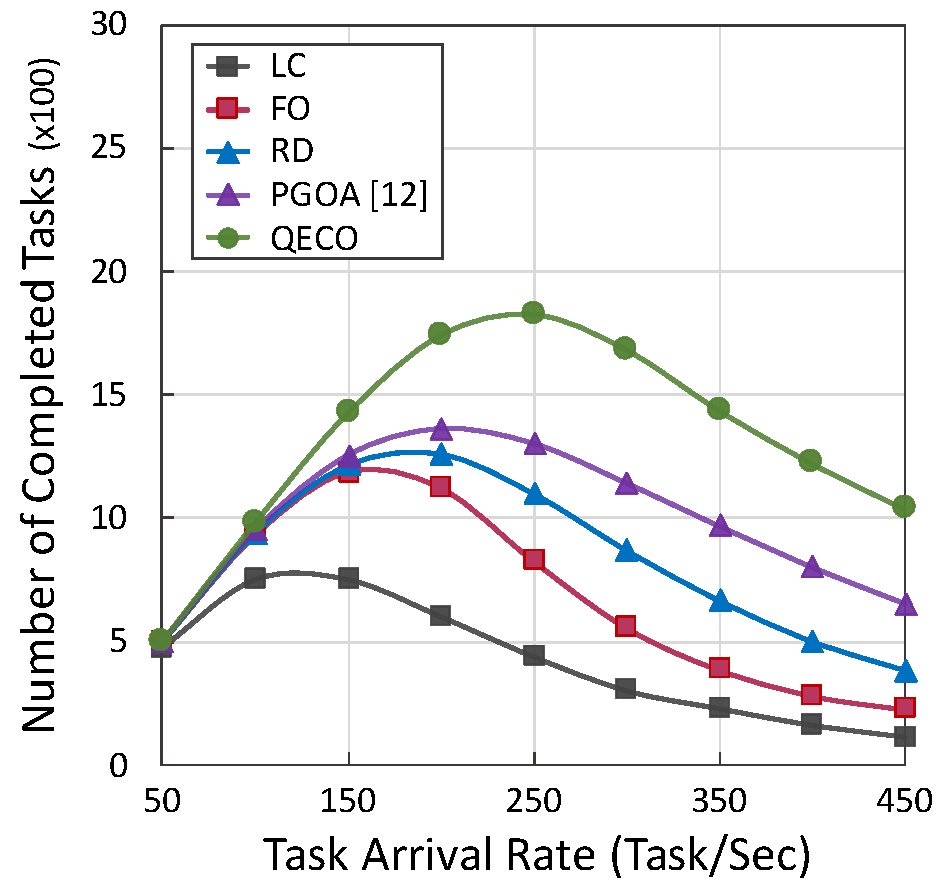
\includegraphics[width=\textwidth]{Fig/completed_tasks_1} 
		\textcolor{white}{i}\hspace{0.6cm}(a)
	\end{minipage}
	\hspace{-0.2cm}
	\begin{minipage}[b]{0.34\linewidth}
		\centering
		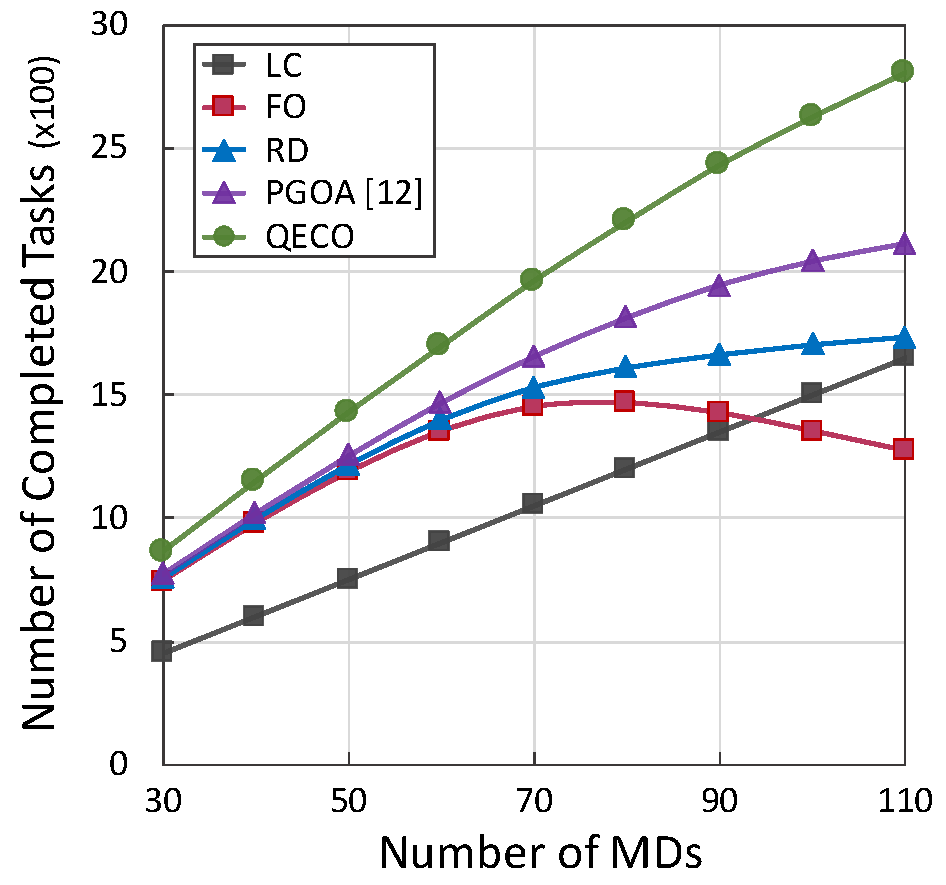
\includegraphics[width=\textwidth]{Fig/completed_tasks_2}
		\textcolor{white}{i}\hspace{0.6cm}(b)
	\end{minipage}
	%\vspace{-0.65cm}
	\caption{The number of completed tasks under different computation workloads: (a) task arrival rate; (b) the number of MDs.}
	\label{chart1}
\end{figure}



\begin{figure}[tbp]
	\centering
	\captionsetup{name=Fig.}
	\begin{minipage}[b]{0.340\linewidth}
		\centering
		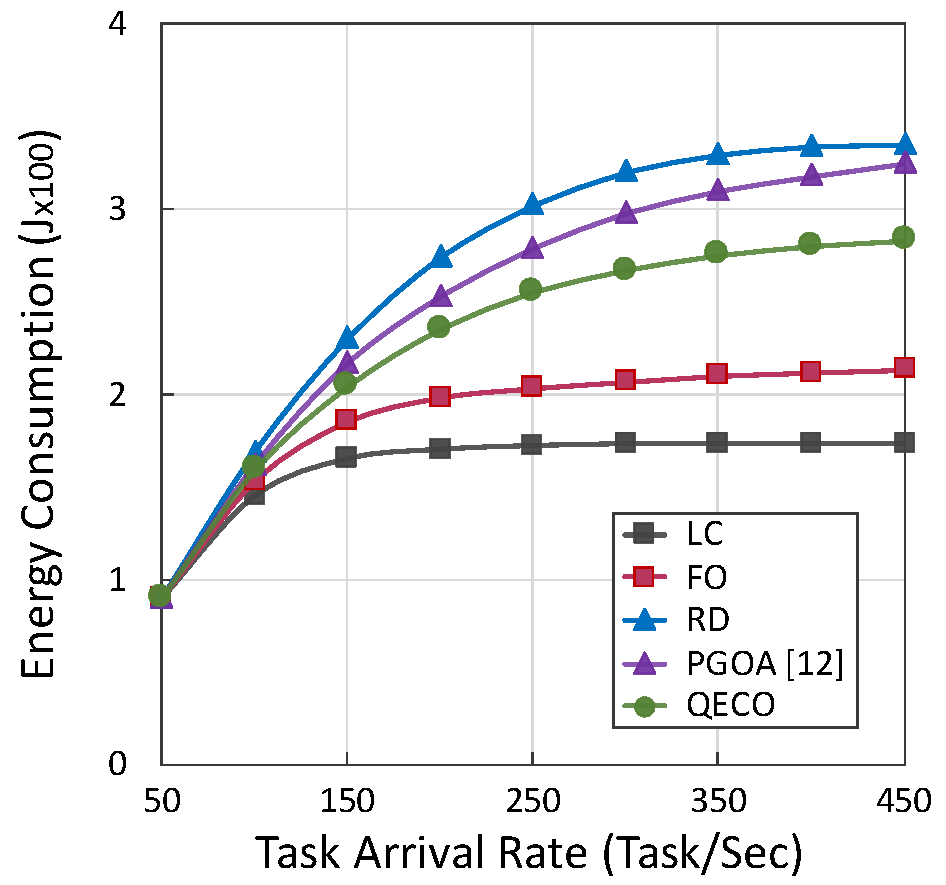
\includegraphics[width=\textwidth]{Fig/energy_1} 		
		\textcolor{white}{i}\hspace{0.6cm}(a)
	\end{minipage}
	%\hspace{-0.2cm}
	\begin{minipage}[b]{0.340\linewidth}
		\centering
		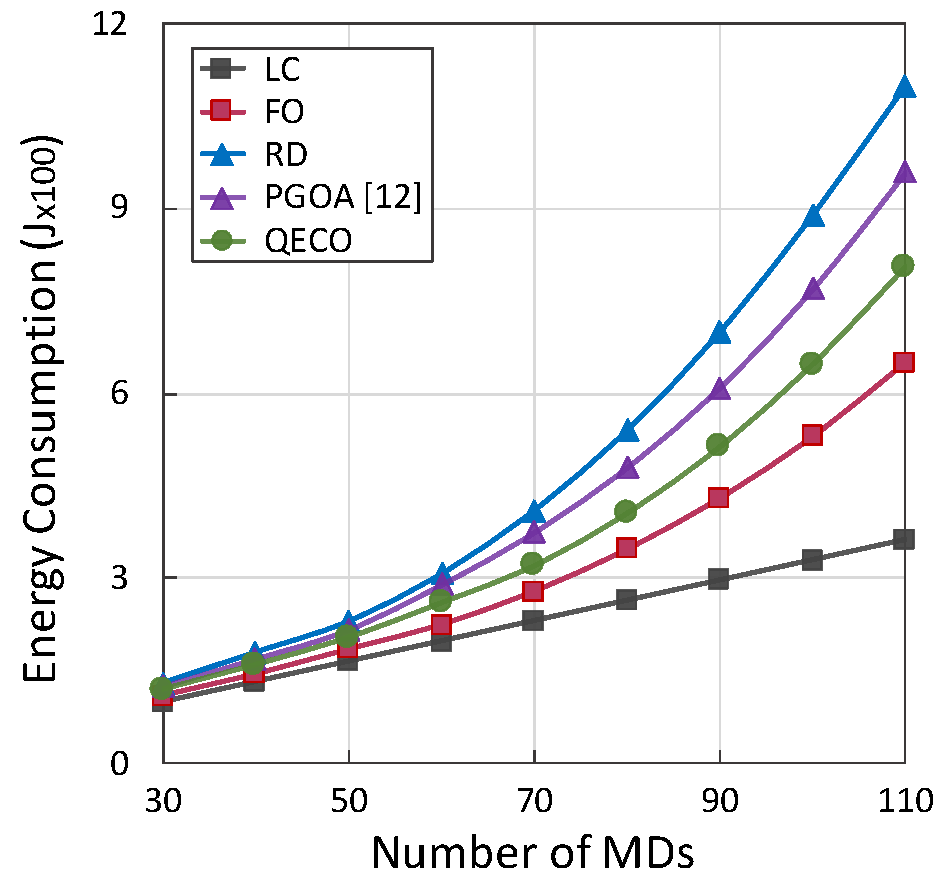
\includegraphics[width=\textwidth]{Fig/energy_2}
		\textcolor{white}{i}\hspace{0.6cm}(b)
	\end{minipage}
	%\vspace{-0.7cm}
	\caption{The overall energy consumption under different computation workloads: (a) task arrival rate; (b) the number of MDs.}
	\label{chart2}
\end{figure}

\begin{figure}[t]
	\centering
	\captionsetup{name=Fig.}
	\begin{minipage}[b]{0.340\linewidth}
		\centering
		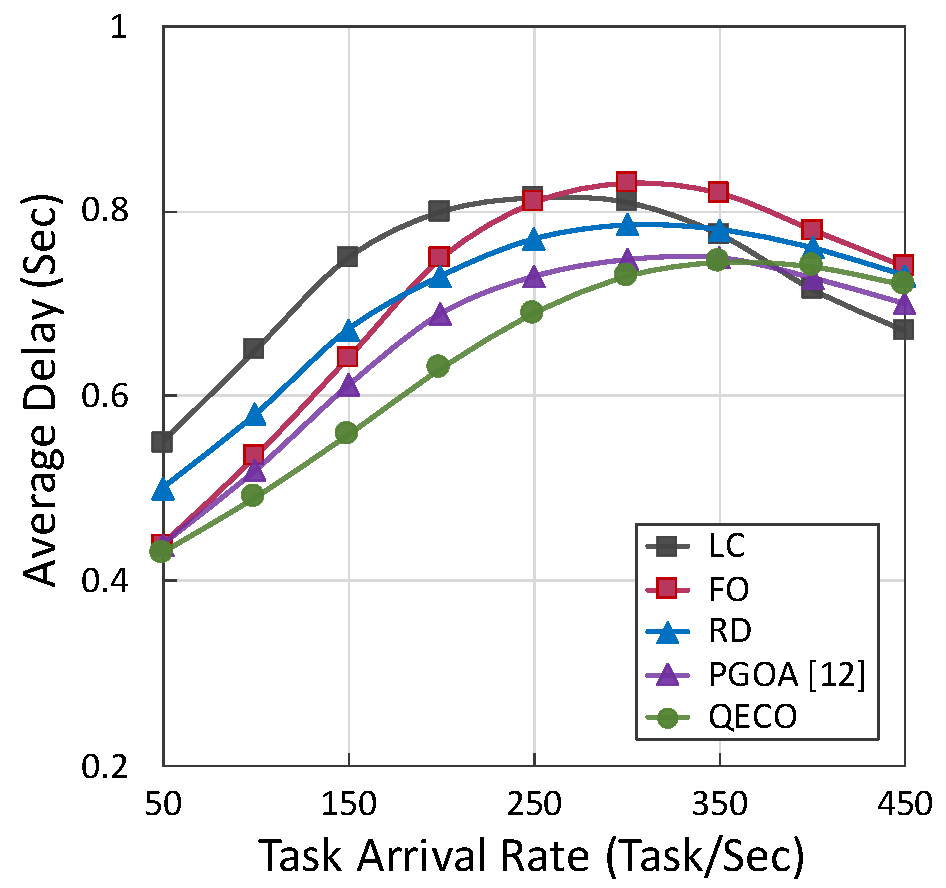
\includegraphics[width=\textwidth]{Fig/delay_1} 		
		\textcolor{white}{i}\hspace{0.6cm}(a)
	\end{minipage}
	\hspace{-0.2cm}
	\begin{minipage}[b]{0.340\linewidth}
		\centering
		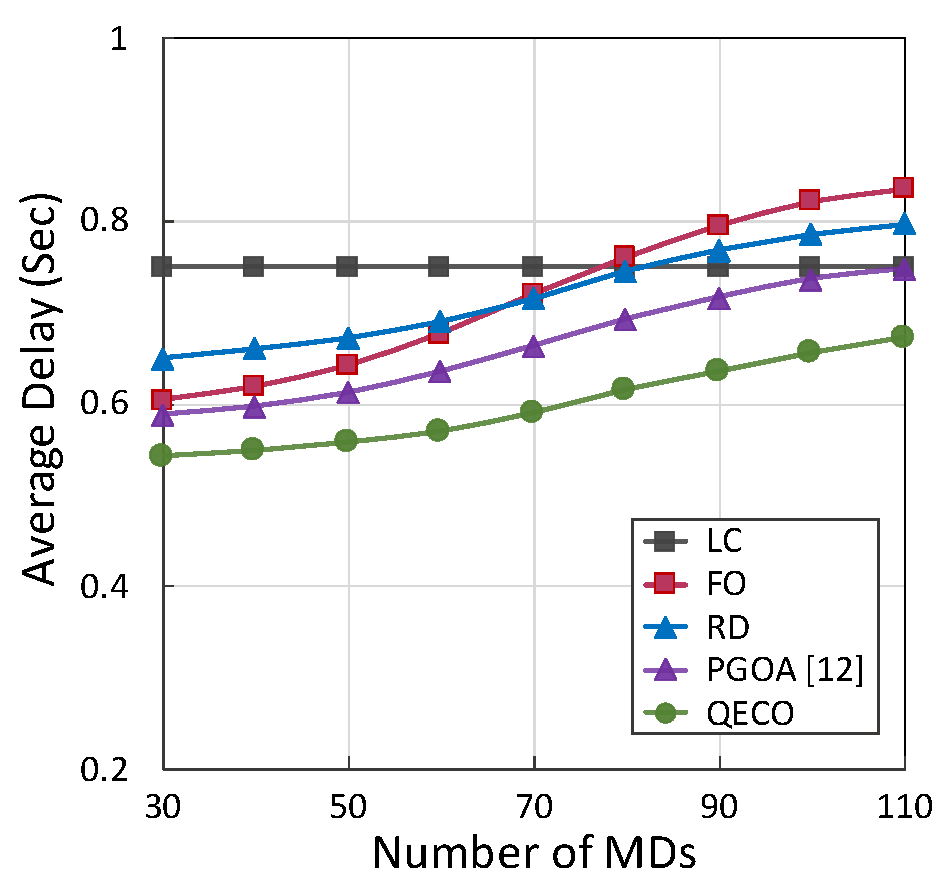
\includegraphics[width=\textwidth]{Fig/delay_2}
		\textcolor{white}{i}\hspace{0.6cm}(b)
	\end{minipage}
	%\vspace{-0.7cm}
	\caption{The average delay under different computation workloads: (a) task arrival rate; (b) the number of MDs.}
	\label{chart3}
\end{figure} 

\begin{figure}[tbp]
	\centering
	\captionsetup{name=Fig.}
	\begin{minipage}[b]{0.340\linewidth}
		\centering
		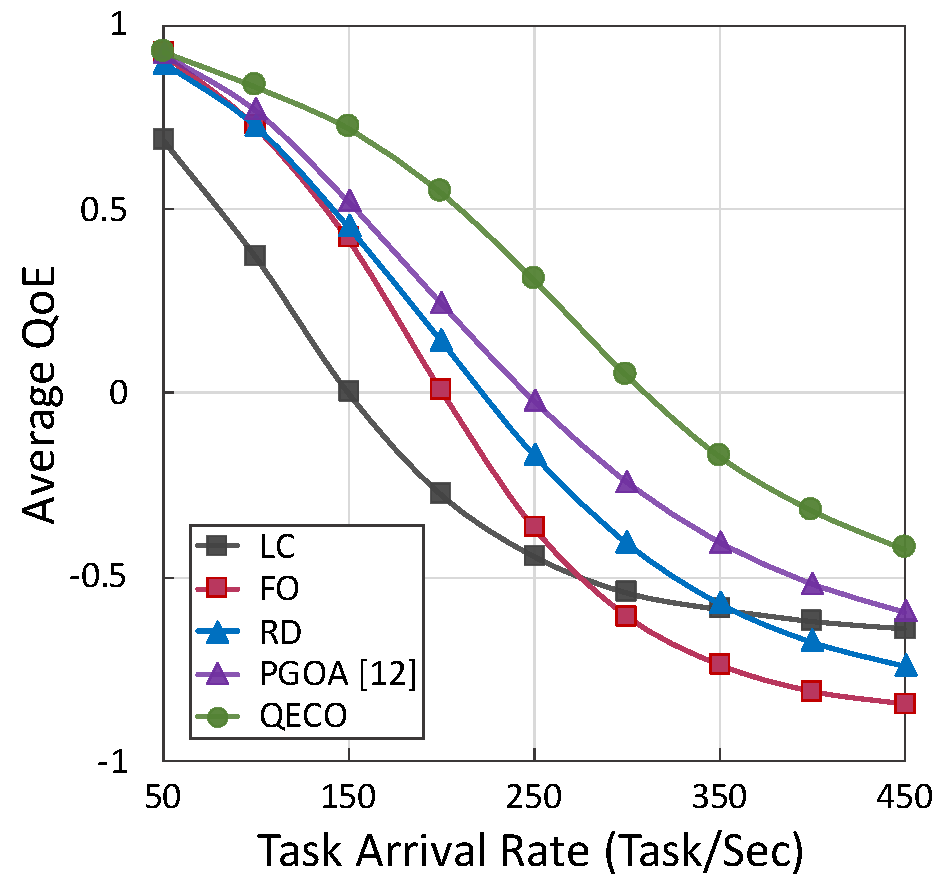
\includegraphics[width=\textwidth]{Fig/qoe_1} 		
		\textcolor{white}{i}\hspace{0.6cm}(a)
	\end{minipage}
	\hspace{-0.2cm}
	\begin{minipage}[b]{0.340\linewidth}
		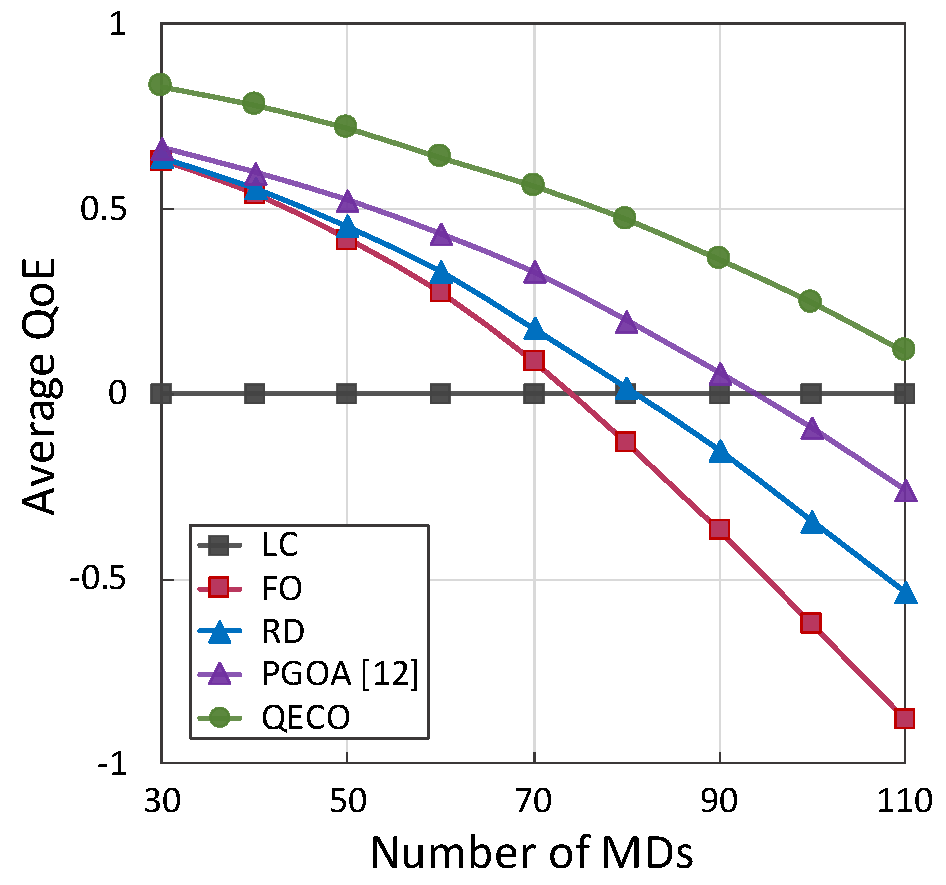
\includegraphics[width=\textwidth]{Fig/qoe_2}
		\textcolor{white}{i}\hspace{0.6cm}(b)
	\end{minipage}
	%\vspace{-0.7cm}
	\caption{The average QoE under different computation workloads: (a) task arrival rate; (b) the number of MDs.}
	\label{chart4}
\end{figure} 





In Fig.~\ref{chart2} (b), an increasing trend in overall energy consumption is observed as the number of MDs increases since the number of resources available in the system increases, which leads to higher energy consumption. The QECO algorithm consistently outperforms RD and PGOA methods in overall energy consumption, especially when there are a large number of MDs. Specifically, QECO demonstrates a 27\% and 16\% reduction in overall energy consumption compared to RD and PGOA, respectively, when the number of MDs increases to 110.

As shown in Fig.~\ref{chart3} (a), the QECO algorithm maintains a lower average delay compared to other methods as the task arrival rate increases from 50 to 350. Specifically, when the task arrival rate is 200, it reduces the average delay by at least 12\% compared to other methods. However, for task arrival rates exceeding 350, QECO may experience a higher average delay compared to some of the other methods. This can be attributed to the fact that the other algorithms drop more tasks while our proposed algorithm is capable of completing a higher number of tasks, potentially leading to an increase in average delay. In Fig.~\ref{chart3} (b), as the number of MDs increases, we observe a rising trend in the average delay. It can be inferred that an increase in computational load in the system can lead to higher queuing delays and computations at ENs. Considering the QECO's ability to schedule workloads, when the number of MDs increases from 30 to 110, it consistently maintains a lower average delay which is at least 8\% less than the other methods.

%Fig. 6 illustrates a performance comparison of methods in terms of energy consumption in the entire system, considering an increase in the task arrival rate and the number of MDs. With efficient decision-making, the DRL-based algorithm achieves lower energy consumption in both cases compared to RD and PGOA. However, it consumes more energy compared to LC and FC. This is because LC only utilizes the MD's computational resources, and FC solely utilizes the transmission link. In Fig. 6(a), when the task arrival rate is low, the energy consumption of all methods is close to each other, and as the task arrival rate increases, the energy consumption of each method also increases. It can be observed that the generation of more computational tasks leads to a continuous increase in energy consumption. When the task arrival rate increases from 0.1 to 0.9, the DRL-based algorithm increases by 20\%, while RD and PGOA increase by at least 30\%. Similarly, in Fig. 6(b), the DRL-based algorithm effectively reduces energy consumption, especially when the number of MDs is large.The DRL-based algorithm demonstrates a 15\% reduction in energy consumption compared to RD and a 30\% reduction compared to PGOA as the number of MDs increases to 110.

%In the following, we delve into the investigation of the overall improvement achieved by the QECO algorithm in comparison to other methods in terms of the average QoE as the task arrival rate and the number of MDs increase. This metric signifies the average advantage created by each method for MDs, including a combination of the values of the previously evaluated metrics (task completion, delay, energy consumption) according to the demands of MDs.

%The average QoE comparison in Fig.~\ref{chart4} (a) indicates the superiority of the QECO algorithm in providing MDs with a better experience. By taking into account the specific demands of MDs for each key performance metric, it consistently achieves a higher average QoE across various values of arrival task rates when compared to other methods. Specifically, when the task arrival rate is moderate (i.e., 250), QECO increases the average QoE by 57\% and 33\% compared to RD and PGOA, respectively. In Fig.~\ref{chart4} (b), As the number of MDs increases, the potential workload on the ENs also rises, leading to a decrease in the average QoE for each method (excluding LC). It can be observed that an increase in the ENs' workload leads to a reduction in the allocated computing capacity for MDs, resulting in a decrease in the average QoE. However, QECO effectively manages the uncertain load at the ENs. When the number of MDs increases to 90, it increases the average QoE by at least 29\% more than the other methods.

We further investigate the overall improvement achieved by the QECO algorithm in comparison to other methods in terms of the average QoE. This metric signifies the advantages MDs obtain by utilizing different algorithms. Fig.~\ref{chart4} (a) shows the average QoE for different values of task arrival rate. This figure indicates the superiority of the QECO algorithm in providing MDs with an enhanced experience. Specifically, when the task arrival rate is moderate (i.e., 250), QECO improves the average QoE by 57\% and 33\% compared to RD and PGOA, respectively. Fig.~\ref{chart4} (b) illustrates the average QoE when we increase the number of MDs. The EN's workload grows when there are a larger number of MDs, leading to a reduction in the average QoE of all methods except LC. However, QECO effectively manages the uncertain load at the ENs. When the number of MDs increases to 90, QECO achieves at least a 29\% higher QoE comparing with the other methods.
It is worth noting that although improvements in each of the QoE factors can contribute to enhancing system performance, it is essential to consider the user's demands in each time slot. Therefore, the key difference between QECO and other methods is that it prioritizes users' demands, enabling it to strike an appropriate balance among them, ultimately leading to a higher QoE for MDs.








We finally delve into the investigation of the convergence performance of the QECO algorithm, which is shown through the average QoE across episodes in Figs.~\ref{chart0} (a) and~\ref{chart0} (b). We explore the impact of two main hyper-parameters on the convergence speed and the converged result of the proposed algorithm. Fig. \ref{chart0} (a) illustrates the convergence of the proposed algorithm under different learning rates, where the learning rate regulates the step size per iteration towards minimizing the loss function. The QECO algorithm achieves an average QoE of 0.77 after around 400 episodes when the learning rate is 0.001, indicating relatively rapid convergence. However, with smaller learning rates (e.g., 0.0001) or larger values (e.g., 0.01),  a slower convergence is observed. Fig. \ref{chart0} (b) shows the convergence of the proposed algorithm under different batch sizes, which refer to the number of sampled experiences in each training round. An improvement in convergence performance is observed as the batch size increases from 4 to 16. However, further increasing the batch size from 16 to 32 does not notably enhance the converged QoE or convergence speed. Hence, a batch size of 16 may be more appropriate for training processes.

\begin{figure}
	\centering
	\captionsetup{name=Fig.}
	\begin{minipage}[b]{0.34\linewidth}
		\centering
		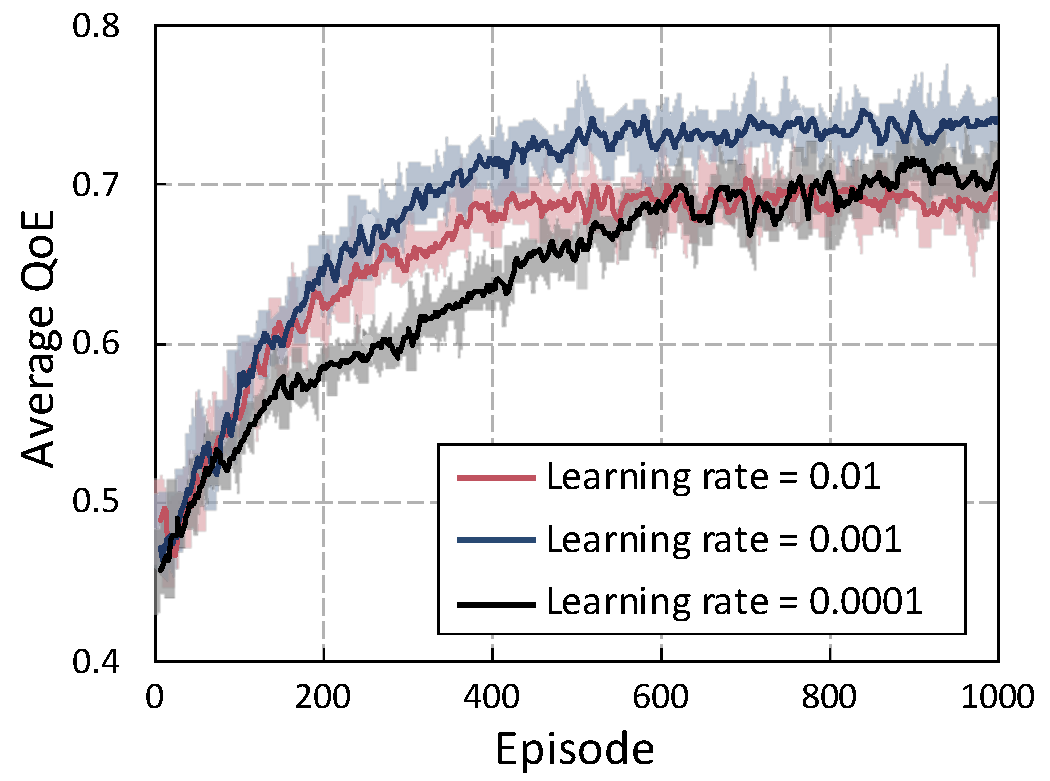
\includegraphics[width=\textwidth]{Fig/conv1_f} 
		\textcolor{white}{i}\hspace{0.4cm}(a)
	\end{minipage}
	\hspace{-0.26cm}
	\begin{minipage}[b]{0.4\linewidth}
		\centering
		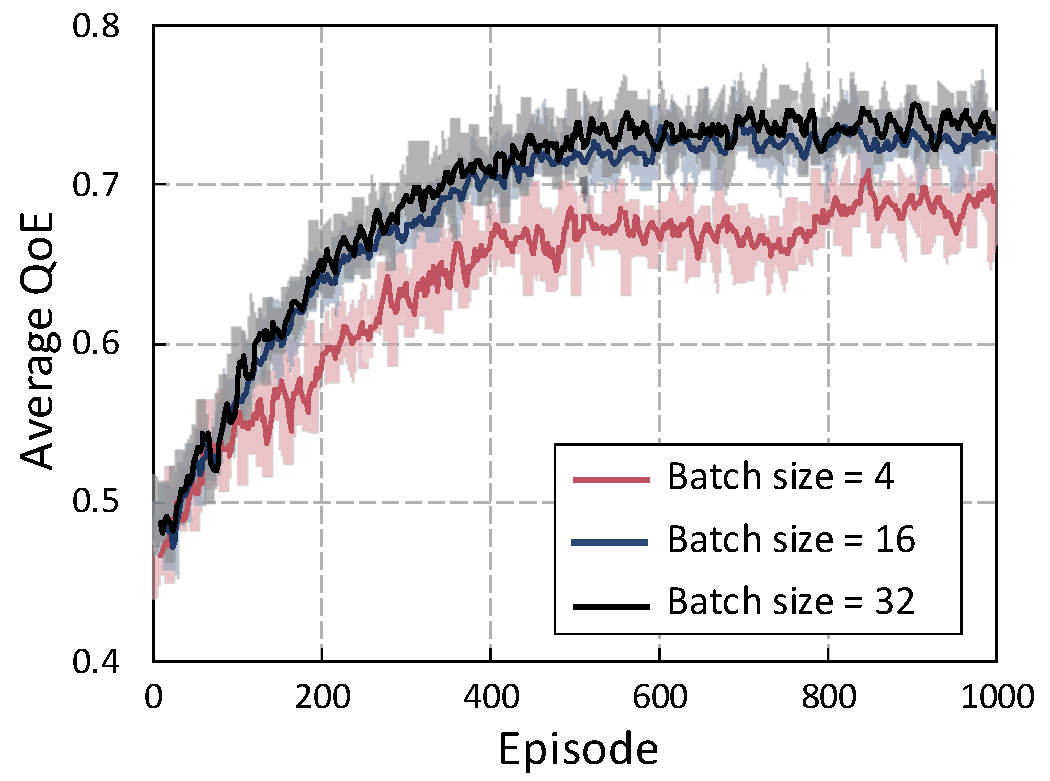
\includegraphics[width=\textwidth]{Fig/conv2_f}
		\textcolor{white}{i}\hspace{0.4cm}(b)
	\end{minipage}
	\vspace{-0.65cm}
	\caption{The convergence of the average QoE across episodes under different hyper-parameters: (a) Learning rate; (b) Batch size.}
	\label{chart0}
\end{figure}




\section{Conclusion}\label{section:VI}
%In this study, our focus was directed towards addressing the challenge of offloading in MEC systems, where strict task processing deadlines and energy constraints adversely impact system performance. To address this challenge, we propose the QECO algorithm specifically designed to empower MDs to make offloading decisions without relying on knowledge about task models or other MDs' offloading decisions. The QECO algorithm not only adapts to the uncertain dynamics of load levels at ENs but also effectively manages the ever-changing system environment. Through extensive simulations, we demonstrate that QECO outperforms several established benchmark techniques. Specifically, it can significantly increase the average user's QoE. This advantage can lead to improvements in key performance metrics, including task completion rate, task delay, and energy consumption, according to the user's demands under different system conditions. 

%There are multiple directions for extend this research. A complementary approach involves extending the simplified task model by considering dependent divisible tasks that correspond to actual computational tasks. This can be achieved by incorporating a call graph~\cite{kwok1996dynamic} representation to develop relationships among task partitions. Furthermore, in order to accelerate the learning of optimal offloading policies, it is beneficial to enable MDs to take advantage of federated learning~\cite{li2020federated} techniques in the training process. This allows MDs to collectively contribute to improving the offloading model and enables continuous learning when new MDs join the network.

In this paper, we focused on addressing the challenge of offloading in MEC systems, where strict task processing deadlines and energy constraints adversely impact system performance. We formulated an optimization problem that aims to maximize the QoE of each MD individually, while QoE reflects the energy consumption and task completion delay. To address the dynamic and uncertain mobile environment, we proposed a QoE-oriented DRL-based computation offloading algorithm called QECO. Our proposed algorithm empowers MDs to make offloading decisions without relying on knowledge about task models or other MDs' offloading decisions. The QECO algorithm not only adapts to the uncertain dynamics of load levels at ENs, but also effectively manages the ever-changing system environment. Through extensive simulations, we showed that QECO outperforms several established benchmark techniques, while demonstrating a rapid training convergence. Specifically, QECO increases the average user's QoE by 37\% compared to an existing work. This advantage can lead to improvements in key performance metrics, including task completion rate, task delay, and energy consumption, under different system conditions and varying user demands.

There are multiple directions for future work. A complementary approach involves extending the task model by considering interdependencies among tasks. This can be achieved by incorporating a task call graph representation. Furthermore, in order to accelerate the learning of optimal offloading policies, it will be beneficial to take advantages of federated learning techniques in the training process. This will allow MDs to collectively contribute to improving the offloading model and enable continuous learning when new MDs join the network.



\newpage




\begin{abstract}
	Mobile edge computing (MEC) is envisioned to address the computation demands of Internet of Things (IoT) devices. However, it is crucial for the MEC to operate in coordination with the cloud tier to achieve a highly scalable IoT system. In addition, IoT devices require regular maintenance to either recharge or replace their batteries which may not always be feasible. Wireless energy transfer (WET) can provide IoT devices a stable source of energy. Nonetheless, proper scheduling of energy harvesting and efficient allocation of computing resources are the key for sustainable operation of these devices. In this paper, we introduce a three-tier wireless powered mobile edge computing (WPMEC) consisting of cloud, MEC servers, and IoT devices. We first formulate a combinatorial optimization problem that aims to minimize the wireless energy transmission. To tackle the complexity of the problem, we use bipartite graph matching and propose a harvest-then-offload mechanism for IoT devices. We also exploit parallel processing to increase the performance of the proposed algorithm. Through numerical experiments, we evaluate the performance of our proposed mechanism. Our results show that the proposed mechanism significantly reduces the required energy for the operation of IoT devices comparing to different offloading policies. \textcolor{blue}{We further show that WiEnTM results in up to 34\% less wireless energy transmission in comparison to an existing work in the literature.}
\end{abstract}

\begin{IEEEkeywords}
	Bipartite graph matching, mobile edge computing (MEC), wireless power transfer (WPT), Internet of Things (IoT)
\end{IEEEkeywords}

\section{Introduction}
\textcolor{blue}{The Internet of Things (IoT) applications (e.g., smart cities \cite{b1}, homes \cite{b3}, and augmented/virtual reality \cite{b11}) are mostly involved with computation-intensive and latency-sensitive tasks. Mobile edge computing (MEC) is a state-of-the-art computation paradigm to address the challenge of insufficient computing resources in IoT networks \cite{b35, b4}. By deploying the edge servers, nearby devices can offload their computation tasks. Dispatching those tasks that require a higher amount of energy will let devices save more energy \cite{b38}. However, as the computation tasks become more and more intensive, coordination with cloud servers will be inevitable \cite{b37}. The three-tier computing models consisting of cloud, edge, and IoT devices are introduced to overcome the aforementioned challenge \cite{b5,b6,b39,b40}.}

\textcolor{blue}{In addition to their restricted computation resources, IoT devices usually have small battery capacities which is mainly due to their small form factor and the constraints of the production cost \cite{b1}.} Thus, their battery needs to be replaced or recharged quite often which may be infeasible or costly in some cases such as toxic \cite{b7} or hard-to-reach environments \cite{b4}. Thanks to the latest developments of radio frequency (RF) enabled wireless energy transfer (WET) technology, a promising solution called wireless powered communication (WPC) has been introduced \cite{b8}. In WPC, wireless devices (WDs) are powered by dedicated energy transmitters (ETs) \cite{b8}. As wireless powered networks do not require replacement or manual recharging of batteries, they have significantly lower maintenance costs. Therefore, these networks are more scalable compared to the battery powered networks in terms of size \cite{b8}. \textcolor{blue}{By combining the advantages of MEC and WPC, the newly emerged wireless powered MEC (WPMEC) holds a major promise to overcome the fundamental hurdles in scalability of the IoT networks \cite{b9,b10,b30,b33}.}

Computation offloading has attracted many research projects in recent years \cite{b5,b39,b40,b11,b13,b29,b26,b28,b32}. \textcolor{blue}{It helps WDs save more energy and reduce the tasks' execution time.} As energy is crucial for the operation and maintenance of wireless powered systems, many of these works are focusing on analyzing and optimizing energy. Aazam \textit{et al.} in \cite{b5} analyzed the energy and performance of a three-tier cloud-edge-IoT offloading model. \textcolor{blue}{In \cite{b39}, authors proposed a scheme that aims to minimize the total cost in terms of energy and delay for a three-tier cloud-edge-IoT system. Gao \textit{et al.} in \cite{b40} proposed an offloading algorithm to minimize an objective called the energy time cost for a three-tier network. Although \cite{b5}, \cite{b39}, and \cite{b40} all benefit from a computationally-scalable three-tier system, IoT devices still rely on battery energy and hence lack the sustainability feature of WPMEC systems.} In \cite{b11}, authors provided a method to maximize energy efficiency in a two-user WPMEC system with user cooperation, non-divisible tasks, and harvest-then-offload TDMA protocol. Wang \textit{et al.} in \cite{b13} presented a heuristic solution to reduce the ET's total transmission energy consumption over a finite horizon in a single-user WPMEC system. In \cite{b29}, authors presented a single-user WPMEC framework with task partitioning to jointly optimize the computation rate and transmit energy. The methods proposed in \cite{b11,b13,b29} are not suitable for larger networks. Zhang \textit{et al.} in \cite{b26} introduced a decentralized game for a multi-user MEC system to optimize the ET's energy and computation costs. Nonetheless, reaching an equilibrium may require a considerable number of iterations. It also needs all WDs to cooperate with each other which may not be feasible in many cases. Huang \textit{et. al} in \cite{b28} proposed an offloading algorithm based on deep reinforcement learning for WPMEC systems with non-divisible tasks to maximize a value function (e.g., computation rate or energy efficiency). \textcolor{blue}{However, the proposed system model is oversimplified and thus less applicable to real-world scenarios.} He \textit{et al.} in \cite{b32} designed a scheduling algorithm to minimize the processing energy consumption for a multi-user WPMEC network with multiple access points (APs) and non-divisible tasks. As a task usually models a program, it consists of a number of interrelated subprograms. It may also include subprograms to send and retrieve data which cannot be offloaded. Therefore, non-divisible task models used in \cite{b11,b26,b28}, and \cite{b32} may not accurately represent real world applications. Additionally, such models cannot properly utilize multiple computing resources.

By considering the challenges of the aforementioned works, the following questions arise:
\begin{enumerate}
	\item \textcolor{blue}{\textit{How can we take advantage of cloud computing in addition to MEC to meet different requirements of IoT applications?}}
	\item \textcolor{blue}{\textit{How can we provide RF energy to enable the battery-less IoT devices operate seamlessly?}}
	\item \textcolor{blue}{\textit{What would be the optimal offloading decision when considering the subtasks' interdependencies?}}
\end{enumerate}

To answer these questions, we propose a novel three-tier WPMEC system with multiple WDs to minimize the ET's total transmitted energy. In the proposed system, we partition tasks into a number of fine-grained subtasks to consider their interdependencies. We design an offloading and scheduling algorithm to be executed efficiently on parallel processors such as graphical processing units (GPUs). \textcolor{blue}{This significantly reduces the execution time of the algorithm.}

\begin{figure}
	\centering
	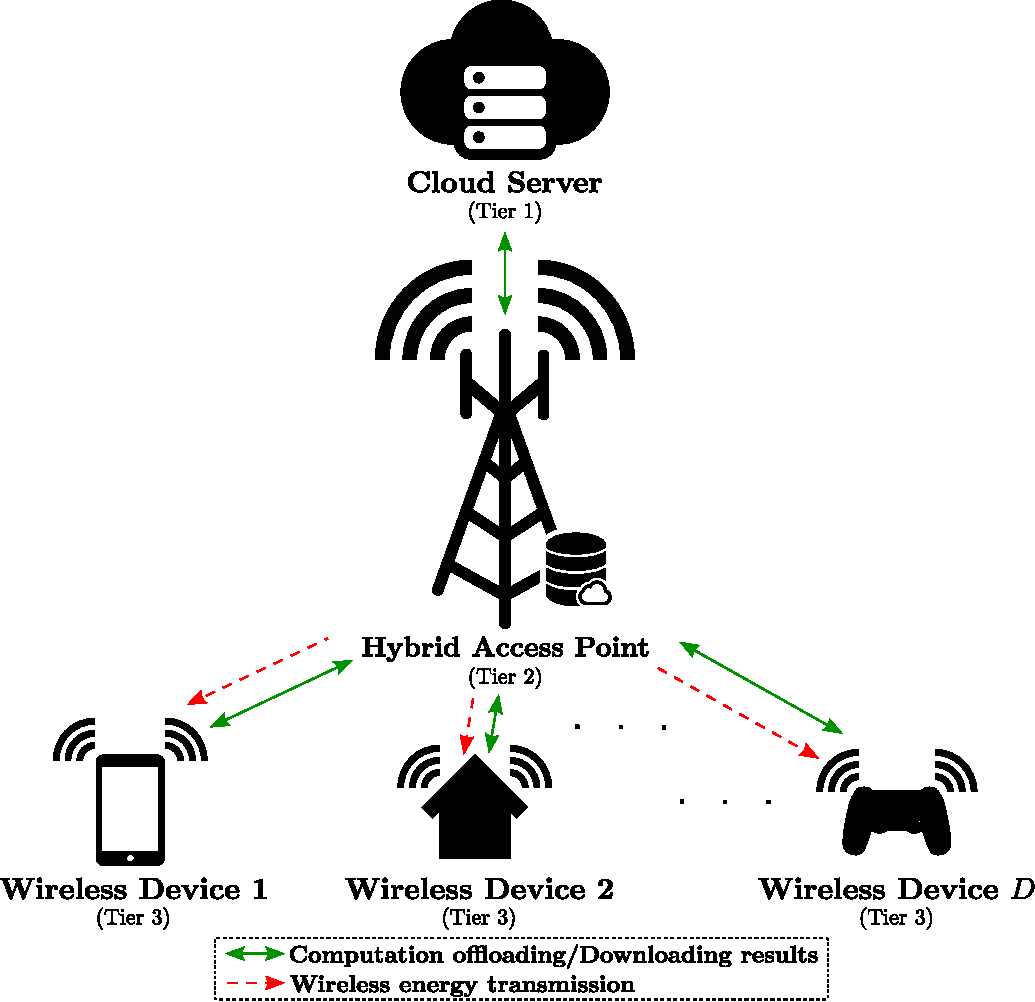
\includegraphics[width=.33\textwidth]{system_model.pdf}
	\caption{Proposed three-tier WPMEC system in an IoT network.}\label{fig1}
\end{figure}

Our main contributions are as follows.
\begin{enumerate}
	\item \textit{Problem formulation}: We formally define the mixed-integer ET's energy minimization (ETEM) problem by deciding on offloading, WET time, and computation scheduling of subtasks for a multi-user three-tier WPMEC system \textcolor{blue}{considering task interdependencies and MEC server computation time.}
	\item \textit{Algorithm design}: We propose wireless energy transmission minimization (WiEnTM) algorithm based on bipartite graph matching. We first study the properties of the problem to decompose it into individual problems for each subtask to make it suitable for the matching algorithm. \textcolor{blue}{By efficiently utilizing parallel processing on decomposed problems, we prove that our proposed algorithm has a logarithmic time complexity with respect to the network size.}
	\item \textit{Performance evaluation}: Extensive numerical experiments are carried out to evaluate the proposed algorithm. Our experiments show major reduction in the WDs' required energy in comparison with baseline offloading policies. \textcolor{blue}{The algorithm also reduces the energy consumption by 34\% for large tasks compared to an existing work \cite{b13}.}
\end{enumerate}

The rest of this paper is organized as follows. In Section II, we first present the MEC system model including the edge and cloud servers and IoT devices. We then present the computation task partitioning model. Section III consists of the energy optimization problem and a step-by-step formulation. In Section IV, we propose our WiEnTM algorithm to efficiently solve the problem. Simulation results are presented in Section V. We conclude the paper in Section VI.

\section{System Model}
In this section, we first introduce the IoT network and computation task models. The IoT network consists of IoT devices and computing servers. The task model represents the subtasks as a directed acyclic graph (DAG) and introduces its associated properties. \textcolor{blue}{Some of the key notations are listed in Table \ref{table1}}.

\subsection{Network Model}
As illustrated in Fig. \ref{fig1}, we consider a three-tier WPMEC system with a cloud server and a hybrid access point (HAP)\footnote{Our analysis can be extended to the case of multiple HAPs by modeling the MEC server as a pool of edge computing servers and considering the fact that each IoT device can only be connected to an HAP.} in a network of multiple WDs. \textcolor{blue}{The HAP is equipped with an MEC server and an ET. MEC and the cloud servers are both able to receive and execute the offloaded tasks and then send the results back to WDs.} ET broadcasts stable RF power to WDs. Thus, with proper scheduling, WDs can sustain their operation by only relying on the harvested energy \cite{b8}. In order to allow multiple WDs to share the same RF-channel, we assume a time-division multiple access (TDMA) protocol for WDs, as inspired by \cite{b11} and \cite{b14}. Moreover, we assume that WDs have half-duplex transmission. As a result, computation offloading cannot be performed simultaneously with energy harvesting \cite{b2}. We thus adopt the \textit{harvest-then-offload} \cite{b2} model of scheduling, as shown in Fig. \ref{fig2}. \textcolor{blue}{In contrast, for the case of full-duplex transmission, scheduling algorithms are categorized as the simultaneous wireless information and power transfer (SWIPT) \cite{b8} mode. However, considering the constraints of the production costs and devices' form factor for battery-less WDs, they usually lack a full-duplex transceiver for energy harvesting and data transmission.}

We now introduce the detailed network model. Let $\mathcal{D}\triangleq\{1,...,D\}$ denote the set of WDs where $D$ indicates the total number of WDs. Each device $d\in\mathcal{D}$ is connected to the HAP and hence, the cloud server, using a wireless interface. \textcolor{blue}{We regard a complete cycle of executing a single subtask for all WDs having a candidate subtask as an \textit{episode}. Each episode jointly models the harvest-then-offload timing, subtasks' deadlines, and TDMA‌ scheduling of WDs.} As shown in Fig. \ref{fig2}, an episode of length $\Gamma$ is divided into two time frames: WET time (i.e., harvesting time) and offloading/local computation time. In the case of offloading, the latter is consisted of three time slots. The first slot is to relocate the task bits from WD $d\in\mathcal{D}$ to the HAP. Then, the task should be either executed on the MEC server or transmitted to the cloud. We consider that the computation time on the cloud server is negligible due to the high computation capacity compared to WDs or the MEC server. Thus, in the case of offloading to the cloud server, the second time slot indicates the time required to send the task data of WD $d\in\mathcal{D}$ from the HAP to the cloud server and then retrieve the processed data. Finally, the results should be transmitted from the HAP back to the corresponding WD in the third time slot.

\textcolor{blue}{Now that we have introduced the network model, we need to provide an approach to calculate the length of episode $\Gamma$. As stated earlier, each episode reflects the requirements of the harvest-then-offload timing and subtask deadlines. Therefore, $\Gamma$ is directly related to the individual subtask deadlines being executed in that episode. In other words, $\Gamma$ can be calculated as the summation of the subtasks' deadlines. In the next section, we will calculate the length of each episode.}

\begin{table}
	\centering
	\caption{{\color{blue}List of key notations}}
	\ContinuedFloat
	\label{table1}
	{\color{blue}\begin{tabular}{ |p{2cm}|p{12cm}|}
			\hline
			\textbf{Symbol} & \textbf{Description} \\
			\hline
			$x^{\text{L}}_{v_d^u}, x^{\text{M}}_{v_d^u}, x^{\text{C}}_{v_d^u}$ & Binary offloading decisions \\
			$\tau_{1,v_d^u}$ & Length of scheduled time for data transmission of subtask $v_d^u$ \\
			$\tau_{2,v_d^u}$ & Length of scheduled time for execution of subtask $v_d^u$\\
			$\tau_{3,v_d^u}$ & Length of scheduled time for retrieving the result of subtask $v_d^u$ \\
			$\tau_0^u$ & WET time in episode $u$\\
			$p^{u}$ & ET's power in episode $u$ \\
			$\Gamma^u$ & Length of episode $u$ \\
			$\mu_{v_d^u}$ & Response time of cloud server for subtask $v_d^u$ \\
			$C_{v_d^u}$ & Number of CPU cycles required for subtask $v_d^u$ \\
			$N_{i,j}$ & Number of bits required to transmit the result of subtask $i$ and $j$ \\
			$g_d$ & Channel gain between WD $d$ and ET \\
			$h_d$ & Channel gain between WD $d$ and MEC server \\
			$\sigma^2$ & Noise power at the HAP \\
			$\eta_d$ & Energy harvesting efficiency of WD $d$ \\
			$\zeta_{d}$ & CPU's effective switched capacitance of WD $d$ \\
			$r_{t,v_d^u}$ & Virtual resource for tier $t$ and subtask $v_d^u$ \\
			$F^{\text{M},\max}$ & Maximum CPU frequency of MEC server \\
			$F^{\text{L},\max}_{d}$ & Maximum CPU frequency of WD $d$ \\
			$P^{\text{ET},\max}$ & ET's maximum transmission power \\
			$P^{\text{AP},\max}$ & AP's maximum transmission power \\
			$P^{\text{WD},\max}_d$ & Maximum transmission power of WD $d$ \\
			$D$ & Number of WDs \\
			$V_d$ & Number of subtasks of WD $d$ \\
			$B_d$ & Bandwidth of WD $d$ \\
			$\mathcal{D}$, $\mathcal{D}^u$ & Set of WDs \\ 
			$\mathcal{U}$ & Set of episodes \\
			$\mathcal{V}_d$ & Set of subtasks of WD $d$ \\
			$\mathcal{R}^{\text{virt}}$ & Set of virtual resources \\
			$\mathcal{I}_{v_d^u}$ & Set of episodes associated to executing prerequisite subtasks of the subtask $v_d^u$ \\
			$\mathcal{J}_{v_d^u}$ & Set of episodes associated to executing subtasks with the subtask $v_d^u$ as their prerequisite \\
			\hline
	\end{tabular}}
\end{table}

\subsection{Task Model}
Generally, there are two main methods for computation offloading: 1) \textit{Binary offloading}, and 2) \textit{partial offloading} which is also known as \textit{program partitioning} \cite{b4}. \textcolor{blue}{In the former method, each task, as an independent unit, is either fully computed locally or offloaded to an MEC server, based on the system constraints such as task arrival time, deadline, and energy harvesting-related constraints.} However, the latter provides a more fine-grained model of tasks by dividing each of them into a number of interrelated subtasks based on the dependencies inside each task \cite{b4}. These subtasks together form a directed, weighted, and acyclic graph known as \textit{task call graph} \cite{b4}. \textcolor{blue}{The partial offloading provides a more realistic model of tasks as it leverages the task call graph to represent each task. This accurately models the call stack of a computer program\footnote{\textcolor{blue}{For instance, \textit{Pyan}\cite{b41} is a Python module that generates the task call graph of a Python code by analysis of its modules and functions.}}} It can also lead to building networks with a higher performance as the optimal offloading decisions are made for each subtask instead of the whole task. Apart from that, by leveraging program partitioning, one can extract and process them in parallel. That being said, it can be a preferred model for many applications including distributively training deep neural networks \cite{b1}, advanced image processing based on parallel processing, and also most of the augmented reality applications \cite{b12}.

\begin{figure}
	\centering
	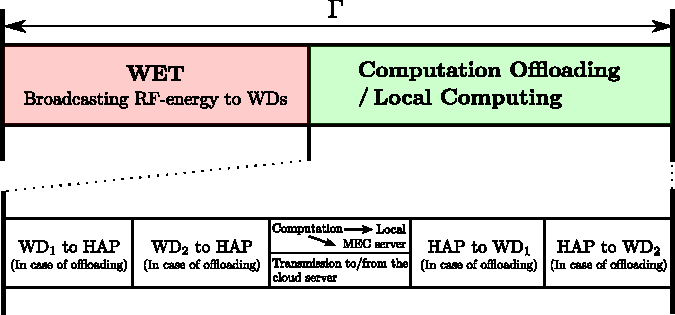
\includegraphics[width=180pt]{TDMA.pdf}
	\caption{\textcolor{blue}{Harvest-then-offload scheduling with TDMA protocol for a system of two WDs. An episode of length $\Gamma$ is divided into two times frames of WET and offloading/local computing. In the case of offloading, the offloading/local computing time frame consists of three slots. The first and last slots are for transmitting the data and retrieving the results, respectively. The second slot is dedicated to the computation in the MEC server or transmission to/from the cloud server.}}\label{fig2}
\end{figure}

\begin{figure}
	\centering
	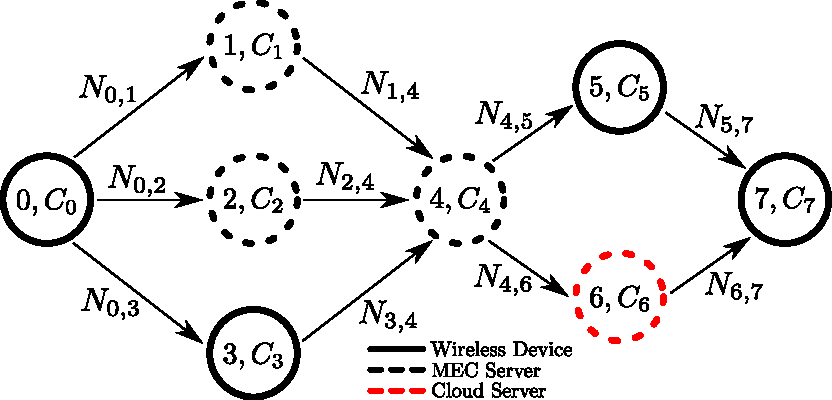
\includegraphics[width=180pt]{task_call_graph.pdf}
	\caption{An example of task call graph with eight subtasks for device $d$. Each parameter $C_{i}$ indicates the computation intensity of subtask $i$ in terms of the number of CPU cycles. Weights $N_{i,j}$ represent the number of bits transferred between subtasks $i$ and $j$.}\label{fig3}
\end{figure}

In this paper, we assume that each device $d\in\mathcal{D}$ has a task which can be partitioned into a number of $V_d$ subtasks using the program partitioning method. We denote $\mathcal{G}_d(\mathcal{V}_d,\mathcal{E}_d)$ as the task call graph of device $d\in\mathcal{D}$ where $\mathcal{V}_d$ indicates the set of vertices which are the subtasks and $\mathcal{E}_d$ denotes the set of edges representing the connection between each two subtasks. Each directed edge $(i,j)\in\mathcal{E}_d$ shows the transmission of the $i$-th subtask output to the $j$-th subtask. An example of this graph with specified computation modes is shown in Fig. \ref{fig3}. For illustration purposes, solid-circled vertices show the subtasks that are computed locally, while vertices with dashed circles correspond to the offloaded subtasks. The black ones are computed on the nearby MEC server and the red one is computed on the remote cloud server. In addition, each subtask $i$ is labeled by a parameter $C_{i}$ which indicates the required CPU cycles to perform the task and represents the task computation intensity. The weight $N_{i,j}$ of the edge from $i$ to $j$ denotes the number of bits required to transmit the result of subtask $i$ to subtask $j$. As the task requires the subtasks to accumulate or send/receive data at the start and end of its procedure, the ones at these ends are executed locally and no offloading decision is made for them \cite{b4}.

\section{Problem Formulation}
This section presents the steps toward formulating the ETEM problem. After providing motivations behind the selection of the objective, we formulate each part of the problem from the objective function to the constraints.

\subsection{Problem Objective}
Due to the high attenuation of RF energy over distances \cite{b8}, WET may require the HAP to consume a considerable amount of energy to provide sustainable operation for WDs. Due to its high cost, it is desired for HAP to consume less energy at the ET. In this paper, we formulate an optimization problem to minimize the total energy consumption of the HAP at the ET by jointly considering computation offloading, scheduling, and power allocation while guaranteeing the task completion and energy constraints. We also adopt the network and task models described in Section II.

Since the proposed WPMEC system consists of multiple WDs and hence multiple task call graphs, we consider the time horizon of the problem to be the number of required episodes to execute the subtasks of all WDs. \textcolor{blue}{We denote $\mathcal{U}\triangleq\{0,...,U-1\}$ as the set of episodes, where $U\triangleq\max_{d\in\mathcal{D}}V_d$  indicates the number of episodes. Note that $V_d$ is obtained from the call graph of the corresponding task.} Therefore, the ET's cumulative energy consumption will be the sum of energy broadcasting over the time horizon. We define $\Gamma^u$, $\tau_0^u$, and $p^u$ as the length of episode $u\in\mathcal{U}$, WET time, and ET's power in episode $u\in\mathcal{U}$, respectively. We will then calculate the HAP's energy consumption at the ET as follows.
\begin{equation}\label{eq2}
	E^{\text{ET}} = \sum_{u\in\mathcal{U}}\tau_0^up^u = \boldsymbol{\tau}_0\boldsymbol{p}^{\intercal},
\end{equation}
where $\boldsymbol{\tau}_0 = \left(\tau_0^u\right)_{u\in\mathcal{U}}$ and $\boldsymbol{p} = \left(p^u\right)_{u\in\mathcal{U}}$ denote the vectors of WET time and ET's transmission power, respectively.

\subsection{Energy harvesting}
In this subsection, we present the energy harvesting-related constraints. \textcolor{blue}{As described earlier, we assume sustainable operation of WDs by only relying on the harvested energy (i.e., battery-less network). Thus, the cumulative energy consumption of the devices on each episode must be no more than their harvested energy.} The required energy of WDs can be divided into two parts: 1) Local computation energy, and 2) energy to send the task's data to the MEC server. We adopt the CPU's dynamic power equation \cite{b2}, \cite{b4}, \cite{b13} to model the local computation energy. We denote $\mathcal{D}^u$ as the set of WDs having a candidate subtask in episode $u\in\mathcal{U}$. We also denote $v_d^u\in\mathcal{V}_d$ as the candidate subtask of WD $d\in\mathcal{D}^u$ to be executed in episode $u\in\mathcal{U}$ and $\tau_{2,v_d^u}$ as the length of time slot scheduled for local computation of this subtask. Therefore, the energy consumption for locally executing subtask $v_d^u\in\mathcal{V}_d$ is
\begin{equation}\label{eq3}
	\begin{aligned}
		E^{\text{LO}}(\tau_{2,v_d^u})=\zeta_d C_{v_d^u}\left(\frac{C_{v_d^u}}{\tau_{2,v_d^u}}\right)^2=\frac{\zeta_d C_{v_d^u}^3}{\left(\tau_{2,v_d^u}\right)^2},&\\
		\forall d\in\mathcal{D}^u, \forall u\in\mathcal{U},&
	\end{aligned}
\end{equation}
where $C_{v_d^u}$ is the number of CPU cycles for executing subtask $v_d^u\in\mathcal{V}_d$ of the corresponding task call graph. Moreover, $\zeta_d$ is the CPU's effective switched capacitance \cite{b13} of device $d\in\mathcal{D}^u$. 

In order to derive the WD energy consumption in case of offloading, we first use the Shannon formula to calculate the transmission rate between the device and MEC server. Assume that $B_d,g_d,q_{v_d^u},$ and $\sigma^2$ denote the spectrum bandwidth, wireless channel gain of device $d\in\mathcal{D}^u$ for data transmission, transmission power for offloading subtask $v_d^u\in\mathcal{V}_d$, and noise power at the HAP, respectively. The transmission rate is then given as
\begin{equation}\label{eq4}
	r_{v_d^u}=B_d\log_2\left(1+\frac{g_dq_{v_d^u}}{\sigma^2}\right),\quad\forall d\in\mathcal{D}^u, \forall u\in\mathcal{U}.
\end{equation}

By utilizing (\ref{eq4}), we will have the following equation for the offloading transmission power.
\begin{equation}\label{eq5}
	q_{v_d^u} = \frac{\sigma^2}{g_d}\left(2^{\frac{r_{v_d^u}}{B_d}}-1\right),\quad\forall d\in\mathcal{D}^u, \forall u\in\mathcal{U}.
\end{equation}

According to the task call graph in Fig. \ref{fig3}, the prerequisite of remotely executing a subtask $v_d^u\in\mathcal{V}_d$ for each device $d\in\mathcal{D}^u$ is to offload the required input data (i.e., the summation of weights of the subtask's input edges) to the MEC server. A time slot with length denoted as $\tau_{1,v_d^u}$ is scheduled for data transmission of subtask $v_d^u\in\mathcal{V}_d$ from device $d\in\mathcal{D}^u$ to the MEC server. We consider $\mathcal{I}_{v_d^u}=\{i\in\mathcal{U}|(v_d^i,v_d^u)\in\mathcal{E}_d\}$ as the set of episodes associated to those subtasks which have an output edge to vertex $v_d^u\in\mathcal{V}_d$. Therefore, by utilizing (\ref{eq5}), we can calculate the offloading energy consumption for each subtask $v_d^u\in\mathcal{V}_d$ as follows.
\begin{equation}\label{eq6}
	\begin{aligned}
		E^{\text{OF}}(\tau_{1,v_d^u}) = \tau_{1,v_d^u}q_{v_d^u} = \frac{\tau_{1,v_d^u}\sigma^2}{g_d}\left(2^{\frac{\sum_{i\in\mathcal{I}_{v_d^u}}{N_{v_d^i,v_d^u}}}{\tau_{1,v_d^u}B_d}}-1\right),&\\
		\forall d\in\mathcal{D}^u, \forall u\in\mathcal{U} &.
	\end{aligned}
\end{equation}

We now determine the amount of harvested energy. Let $\eta_d$ and $h_d$ denote the energy harvesting efficiency of WD $d\in\mathcal{D}$ and channel gain between the WD and ET, respectively. The harvested energy during each episode $u\in\mathcal{U}$, denoted as $E^{\text{EH}}(\tau_0^u,p^u)$, is
\begin{equation}\label{eq7}
	E^{\text{EH}}(\tau_0^u,p^u) = \eta_dh_d\tau_0^up^u,\quad\forall u\in\mathcal{U}.
\end{equation}

By denoting $P^{\text{ET}, \max}$ as the maximum power ET can transmit, we will have the following constraint on $p^u$.
\begin{equation}\label{eq7_1}
	0\leq p^u\leq P^{\text{ET}, \max},\quad\forall u\in\mathcal{U}.
\end{equation}

We denote $x^{\text{L}}_{v_d^u}$, $x^{\text{M}}_{v_d^u}$, and $x^{\text{C}}_{v_d^u}$ as binary variables that indicate the offloading decision of subtask $v_d^u$ of device $d\in\mathcal{D}^u$ in episode $u\in\mathcal{U}$. If $x^{\text{L}}_{v_d^u}=1$, the subtask is performed locally while $x^{\text{M}}_{v_d^u}=1$ indicates that the subtask is offloaded to the MEC server and $x^{\text{C}}_{v_d^u}=1$ means that it is offloaded to the cloud server. As stated earlier, we consider that the proposed WPMEC system is fully wireless powered. As a result, the consumed energy of each WD should be at most equal to its harvested energy. Therefore, by utilizing (\ref{eq3}), (\ref{eq6}), and (\ref{eq7}), we have the following constraint.
\begin{equation}\label{eq8}
	\begin{aligned}
		E^{\text{LO}}(\tau_{2,v_d^u})x^{\text{L}}_{v_d^u} + E^{\text{OF}}(\tau_{1,v_d^u})\left(x^{\text{M}}_{v_d^u}+x^{\text{C}}_{v_d^u}\right) \leq E^{\text{EH}}(\tau_0^u,p^u),& \\
		\forall d\in\mathcal{D}^u, \forall u\in\mathcal{U}.&
	\end{aligned}
\end{equation}
Note that the excessive harvested energy cannot be stored for future use.

\subsection{Harvest-then-offload TDMA scheduling}
We adopt the harvest-then-offload scheduling mechanism to enable WDs with half-duplex transmission to execute or offload their computation tasks. We also leverage a TDMA protocol for scheduling multiple WDs according to Fig. \ref{fig2}. We consider that an episode of WET and task execution for all WDs should not exceed the length of episode $\Gamma^u$. Therefore, by assuming $u\in\mathcal{U}$ as the episode, the following constraints should be satisfied.
\begin{equation}\label{eq9}
	\tau_0^u + \sum_{d\in\mathcal{D}^u}\left(\tau_{1,v_d^u} +\tau_{2,v_d^u}+\tau_{3,v_d^u}\right) \leq \Gamma^u,\quad\forall u\in\mathcal{U},
\end{equation}
\begin{equation}\label{eq9_1}
	0\leq\tau_0^u\leq\Gamma^u,\quad\forall u\in\mathcal{U},
\end{equation}
where $\tau_{3,v_d^u}$ denotes the length of scheduled time for retrieving the results of subtask $v_d^u\in\mathcal{V}_d$ from the MEC server. \textcolor{blue}{It is worth noting that inequality (\ref{eq9}) also enforces a hard deadline for each cycle of subtasks' execution in each episode. Thus, the total execution time of each task generated by WDs is constrained. This way, we can address the requirements of latency-sensitive tasks as well. Also, it can be concluded that $\Gamma^u$ is a key factor in the optimal value of the ETEM problem. A longer episode (i.e., larger $\Gamma^u$) provides more time for execution of the tasks. In fact, this will enlarge the feasible region of the ETEM optimization problem and enhances the energy-efficiency of the algorithm.}

As illustrated in Fig. \ref{fig2}, in the case of offloading to the MEC server (i.e., $x^{\text{M}}_{v_d^u}=1$) or cloud server (i.e., $x^{\text{C}}_{v_d^u}=1$), the time $\tau_{1,v_d^u}$ must be at most $\Gamma^u$. The figure also shows that if the subtask is executed locally (i.e., $x^{\text{L}}_{v_d^u}=1$ and $x^{\text{M}}_{v_d^u}=x^{\text{C}}_{v_d^u}=0$), $\tau_{1,v_d^u}$ should be equal to zero. Therefore, the following constraint holds.
\begin{equation}\label{eq10}
	\tau^{\min}_{1,v_d^u}\leq\tau_{1,v_d^u}\leq \tau^{\max}_{1,v_d^u},\quad\forall d\in\mathcal{D}^u, \forall u\in\mathcal{U},
\end{equation}
where $\tau^{\min}_{1,v_d^u}\triangleq\frac{\sum_{i\in\mathcal{I}_{v_d^u}}N_{v_d^i,v_d^u}}{B_d\log_2\left( 1+\frac{g_dP^{\text{WD}, \max}_d}{\sigma^2}\right)}\left(x^{\text{M}}_{v_d^u} + x^{\text{C}}_{v_d^u}\right)$ and  $\tau^{\max}_{1,v_d^u}\triangleq\Gamma^u\left(x^{\text{M}}_{v_d^u} + x^{\text{C}}_{v_d^u}\right)$ are obtained using (\ref{eq4}). In addition, $P^{\text{WD}, \max}_d$ denotes the maximum transmission power for WD $d\in\mathcal{D}$.

Constraints (\ref{eq8}) and (\ref{eq10}) address a tradeoff between the energy consumption and the transmission duration in the WDs. Above statements are also held for time $\tau_{3,v_d^u}$. Thus, we introduce the following constraint:
\begin{equation}\label{eq11}
	\tau^{\min}_{3,v_d^u} \leq \tau_{3,v_d^u} \leq \tau^{\max}_{3,v_d^u},\quad\forall d\in\mathcal{D}^u, \forall u\in\mathcal{U},
\end{equation}
where
$\tau^{\min}_{3,v_d^u}\triangleq\frac{\sum_{j\in\mathcal{J}_{v_d^u}}N_{v_d^u,v_d^j}}{B_d\log_2\left( 1+\frac{g_dP^{\text{AP}, \max}}{\sigma^2}\right)}\left(x^{\text{M}}_{v_d^u} + x^{\text{C}}_{v_d^u}\right), $ $\tau^{\max}_{3,v_d^u}\triangleq\Gamma^u\left(x^{\text{M}}_{v_d^u} + x^{\text{C}}_{v_d^u}\right),$  $\mathcal{J}_{v_d^u}=\{j\in\mathcal{U}|(v_d^u,v_d^j)\in\mathcal{E}_d\},$ and $P^{\text{AP}, \max}$ denotes the maximum AP's transmission power.

It is also worth noting that according to Fig. \ref{fig2}, in the case of local computation, there will not be any time required for data transmission between the MEC server and the corresponding WD. Thus, we have the following constraints for the first and last subtasks of each task call graph.
\begin{equation}\label{eq12_1}
	\tau_{1,v_d^0} = \tau_{3,v_d^0} = \tau_{1,v_d^{V_d-1}} = \tau_{3,v_d^{V_d-1}} = 0,\quad\forall d\in\mathcal{D},
\end{equation}
\begin{equation}\label{eq12_2}
	x^{\text{M}}_{v_d^0} = x^{\text{C}}_{v_d^0} = x^{\text{M}}_{v_d^{V_d-1}} = x^{\text{C}}_{v_d^{V_d-1}} = 0,\quad\forall d\in\mathcal{D},
\end{equation}
where $v_d^0,v_d^{V_d-1}\in\mathcal{V}_d$ indicate the first and last subtasks of device $d\in\mathcal{D}$, respectively.

We denote $F^{\text{L},\max}_{d}$ as the maximum CPU frequency of device $d\in\mathcal{D}$. We also denote $F^{\text{M},\max}$ as the maximum CPU frequency of the MEC server. We consider $C_{v_d^u}$ as the number of CPU cycles for executing a subtask $v_d^u\in\mathcal{V}_d$ on device $d\in\mathcal{D}^u$. Thus, $\tau_{2,v_d^u}$ will be at least $C_{v_d^u}/F^{\text{L},\max}_{d}$ if the subtask is locally computed or $C_{v_d^u}/F^{\text{M},\max}$ in the case of offloading to the MEC server. However, as the cloud servers mostly benefit from powerful processors, we omit the processing delay if the subtask is offloaded to the cloud server. Therefore, the scheduling time $\tau_{2,v_d^u}$ is affected by the server's load and also the round-trip and transmission delay from the MEC server to the cloud. We refer this as the response time which is denoted as $\mu_{v_d^u}\geq 0$ for each device $d\in\mathcal{D}^u$ and episode $u\in\mathcal{U}$. As a result, we have
\begin{equation}\label{eq13}
	\tau^{\min}_{2,v_d^u} \leq \tau_{2,v_d^u} \leq\Gamma^u,\quad\forall d\in\mathcal{D}^u, \forall u\in\mathcal{U},
\end{equation}
where $\tau^{\min}_{2,v_d^u}\triangleq\frac{C_{v_d^u}}{F^{\text{L},\max}_{d}}x^{\text{L}}_{v_d^u} + \frac{C_{v_d^u}}{F^{\text{M},\max}}x^{\text{M}}_{v_d^u} +
\mu_{v_d^u}x^{\text{C}}_{v_d^u}$. The response time $\mu_{v_d^u}$ is estimated by the MEC server at the beginning of each episode $u\in\mathcal{U}$ for each WD $d\in\mathcal{D}^u$.

\subsection{ET's Energy Minimization (ETEM) Problem}
To formulate the problem, we first define three offloading decision vectors for cloud, edge, and local computation as $\boldsymbol{x}^\text{C} = \left(x^{\text{C}}_{v_d^u}\right)_{\sum_{d\in\mathcal{D}}V_d}$, $\boldsymbol{x}^{\text{M}} = \left(x^{\text{M}}_{v_d^u}\right)_{\sum_{d\in\mathcal{D}}V_d}$, and $\boldsymbol{x}^{\text{L}} = \left(x^{\text{L}}_{v_d^u}\right)_{\sum_{d\in\mathcal{D}}V_d}$, respectively. We also define decision matrix $\boldsymbol{X} = \left(x_{t,v_d^u}\right)_{3\times \sum_{d\in\mathcal{D}}V_d} = \left(\boldsymbol{x^\text{C}};\boldsymbol{x^\text{M}};\boldsymbol{x^\text{L}}\right)$, where each row corresponds to a tier number $t\in\{1,2,3\}$. We also define $\boldsymbol{T} = (\tau_{m,v_d^u})_{3\times \sum_{d\in\mathcal{D}}V_d}$ as the computation scheduling matrix with $m\in\{1,2,3\}$ representing the time frame number. We can now formulate the ETEM problem as follows.
\begin{subequations}
	\begin{alignat}{4}
		\text{ETEM: }\displaystyle{\minimize_{\boldsymbol{X},\boldsymbol{p},\boldsymbol{\tau}_0,\boldsymbol{T}}}\quad & \boldsymbol{\tau}_0\boldsymbol{p}^{\intercal} \label{p1a}\\
		%
		\textrm{subject to} \quad & \text{constraints } (\ref{eq7_1})\text{--}(\ref{eq13}), \label{p1b}\\
		%
		\begin{split}
			&x^{\text{L}}_{v_d^u} + x^{\text{M}}_{v_d^u} + x^{\text{C}}_{v_d^u} = 1,\\
			%
			&\quad\quad\forall d\in\mathcal{D}^u, \forall u\in\mathcal{U}, \label{p1c}
			%
		\end{split}\\
		\begin{split}
			&x^{\text{L}}_{v_d^u}, x^{\text{M}}_{v_d^u}, x^{\text{C}}_{v_d^u}\in\left\{0,1\right\},\\
			%
			&\quad\quad\forall d\in\mathcal{D}^u, \forall u\in\mathcal{U}. \label{p1d}
			%
		\end{split}
	\end{alignat}
\end{subequations}

ETEM is a mixed-integer optimization problem which is intractable. In the next section, we will propose our algorithm called WiEnTM to efficiently solve the problem by leveraging bipartite graph matching and parallel processing\cite{b16}.

\section{Wireless Energy Transmission Minimization (WiEnTM) Algorithm}

In this section, we propose our parallel WiEnTM algorithm to solve the ETEM problem using bipartite graph matching. We also analyze the time complexity of each parallel block of the algorithm.

\subsection{Bipartite Graph Matching}
Matching in graph theory can provide a tractable approach to combinatorial optimization problems \cite{b17}. Matching theory has been widely used for resource allocation in wireless networks where the users and resources are modeled as a bipartite graph \cite{b16}, \cite{b17}. In this graph, users are connected to resources via edges. Each edge is associated with a weight which represents the cost of using the corresponding resource. A subset of edges associated with a feasible resource allocation is called a \textit{matching}. The goal is to find the minimum weighted graph matching.


\begin{figure*}[ht]
	\centering
	\begin{subfigure}{.21\textwidth}
		\centering
		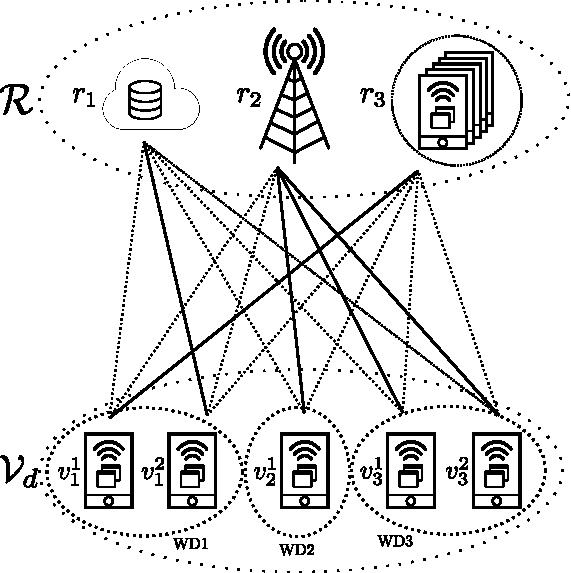
\includegraphics[height=\linewidth]{matching1.pdf}
		\caption{}
		\label{fig:4a}
	\end{subfigure}\hspace{8mm}
	\begin{subfigure}{.21\textwidth}
		\centering
		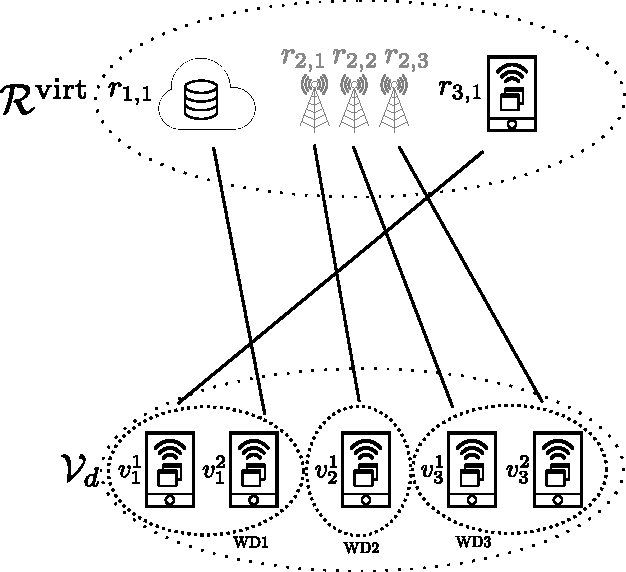
\includegraphics[height=\linewidth]{matching2.pdf}
		\caption{}
		\label{fig:4b}
	\end{subfigure}
	
	\caption{An example for matching bipartite graph of subtasks $\mathcal{V}_d$ and computation resources $\mathcal{R}$. Set $\mathcal{R}$ contains resources $r_1$ (i.e., cloud servers), $r_2$ (i.e., MEC servers), and $r_3$ (i.e., local devices). a) Many-to-one matching. b) Equivalent one-to-one matching by utilizing virtual resources $\mathcal{R}^{\text{virt}}$ where each $r_{t,v_d^u}$ is related to tier number $t\in\{1,2,3\}$ and subtask $v_d^u$.} \label{fig:4}
\end{figure*}

The bipartite graph in Fig. \ref{fig:4} provides an example of matching problem in the proposed WPMEC system. In Fig. \ref{fig:4a}, each subtask $v_d^u\in\mathcal{V}_d$ of device $d\in\mathcal{D}^u$ in episode $u\in\mathcal{U}$ is matched with computation resources of set $\mathcal{R}$ which consists of cloud, MEC server, and local devices. It is important to note that device $d$ can only be matched with itself or cloud/edge resources not other devices.

\textcolor{blue}{To leverage the matching algorithm, we need to calculate the cost of each matching between subtasks and computing resources. To accomplish this, we first transform the ETEM problem into an equivalent simplified problem. We then show that the transformed problem is decomposable, and the resultant decomposed problems are still equivalent to the ETEM problem.}

For each matching, the binary decision variables $x_{v_d^u}^{\text{L}}$, $x_{v_d^u}^{\text{M}}$, and $x_{v_d^u}^{\text{C}}$ will have known values (e.g., matching subtask $v_d^u\in\mathcal{V}_d$ with the cloud resource will result in $x_{v_d^u}^{\text{C}} = 1$ and $x_{v_d^u}^{\text{L}}=x_{v_d^u}^{\text{M}}=0$). However, the ETEM problem is still non-convex even with eliminating binary variables. This is due to the term $\tau_0^up^u$ which is neither a convex nor concave function of $\tau_0^u$ and $p^u$. For the sake of resolving this issue, we present the following theorem.

\begin{theorem}
	Given a matching (i.e., particular values of binary variables $x^{\text{L}}_{v_d^u}$, $x^{\text{M}}_{v_d^u}$, and $x^{\text{C}}_{v_d^u}$), ETEM can be transformed into a convex optimization problem.
\end{theorem}
\begin{IEEEproof}
	Refer to Appendix A.
\end{IEEEproof}

We now transform the ETEM problem with the change of variable $\varepsilon^u=\tau_0^up^u$ into a more tractable form. This helps us calculate the edge weights in the matching graph. In order to accomplish this, it is required to decompose the aforementioned problem into problems for each subtask $v_d^u\in\mathcal{V}_d$ of device $d\in\mathcal{D}$ in episode $u\in\mathcal{U}$. We first provide two important remarks as follows.

\begin{remark}
	The optimal value of variable $\tau_{3,v_d^u}$ will be
	\begin{equation}\label{eq18}
		\tau_{3,v_d^u}^{\ast} \triangleq \tau_{3,v_d^u}^{\min},\quad\forall d\in\mathcal{D}^u, \forall u\in\mathcal{U}.
	\end{equation}
\end{remark}
\noindent The above equation eliminates constraint (\ref{eq11}).

Variable $\tau_{3,v_d^u}$ is only present in constraints (\ref{eq9}) and (\ref{eq11}). Since (\ref{eq9}) forces a hard deadline on the scheduling times, it is desirable for $\tau_{3,v_d^u}$ to have the smallest possible value which is dictated by constraint (\ref{eq11}). Therefore, at the optimal point of ETEM problem, \ref{eq18} will be achieved.

\begin{remark}
	We can calculate the transmitted wireless energy during each episode $u\in\mathcal{U}$ as
	\begin{equation}\label{eq19}
		\varepsilon^u = \max_{d\in\mathcal{D}^u}\left\{\frac{E^{\text{LO}}(\tau_{2,v_d^u})x^{\text{L}}_{v_d^u}}{\eta_d h_d} + \frac{E^{\text{OF}}(\tau_{1,v_d^u})\left(x^{\text{M}}_{v_d^u}+x^{\text{C}}_{v_d^u}\right)}{\eta_d h_d}\right\},
	\end{equation}
	where $v_d^u\in\mathcal{V}_d$ is the candidate subtask of device $d\in\mathcal{D}^u$ that is being executed in episode $u\in\mathcal{U}$.
\end{remark}

We know that the objective of the ETEM problem is to minimize the wireless energy transmission. This minimum value must meet the energy requirements of all WDs. Therefore, it is the maximum energy consumption among WDs in each episode $u\in\mathcal{U}$. Using the above remark, we can rewrite the objective function and eliminate constraint (\ref{eq8}).

Using (\ref{eq19}), we can transform ETEM into a minimax optimization problem but it may still be difficult to solve when there are large number of WDs. We know that constraint (\ref{eq9}) is creating a dependency between subtasks. By rewriting this constraint for each subtask, we will be able to reduce this minimax optimization problem into a number of independent problems. As a result, the ETEM problem will convert into a minisum optimization problem \cite{b18} which is easier to solve.

In order to eliminate the aforementioned dependency in constraint (\ref{eq9}), we first consider a given value for the WET time $\tau_0^u$ which satisfies constraint (\ref{eq9_1}). Thus, the ET's transmitted energy will only depend on $p^u$. There are iterative methods to calculate the appropriate value of $\tau_0^u$ such as the one proposed in \cite{b2}. By decomposing the summation on the left-hand side of (\ref{eq9}), this constraint can be rewritten for each subtask $v_d^u\in\mathcal{V}_d$. We first introduce a new parameter $0\leq\beta_{v_d^u}\leq|\mathcal{D}^u|$ which reflects the priority, computation complexity, or input/output size of each subtask $v_d^u\in\mathcal{V}_d$. We then introduce the following constraint.
\begin{equation}\label{eq28}
	\tau_{1,v_d^u} + \tau_{2,v_d^u} \leq \frac{\beta_{v_d^u}}{|\mathcal{D}^u|}\left(\Gamma^u-\tau_0^u\right) - \tau_{3,v_d^u}^{\ast}.
\end{equation}

We now reconstruct (\ref{eq9}) using (\ref{eq28}). To do so, we accumulate each side of (\ref{eq28}) over all WDs in $\mathcal{D}$ and choose $\beta_{v_d^u}$ such that
\begin{equation}\label{eq27}
	\sum_{d\in\mathcal{D}^u}\beta_{v_d^u} \leq 	|\mathcal{D}^u|,\quad\forall u\in\mathcal{U}.
\end{equation}

It can be easily shown that when the above condition holds, constraint (\ref{eq28}) ensures that constraint (\ref{eq9}) is met. Moreover, in the case of equality, constraints (\ref{eq9}) and (\ref{eq28}) will be equivalent. \textcolor{blue}{We will analyze the effect of $\beta_{v_d^u}$ on the optimal solution in Section V.}

For ease of exposition, we now define the following two functions for each $v_d^u\in\mathcal{V}_d$ assuming $x^{\text{L}}_{v_d^u}$, $x^{\text{M}}_{v_d^u}$, and $x^{\text{C}}_{v_d^u}$ are given.
\begin{equation}\label{eq20}
	\begin{aligned}
		e_1(\tau_{1,v_d^u}) &\triangleq \frac{E^{\text{OF}}_{v_d^u}\left(x^{\text{M}}_{v_d^u}+x^{\text{C}}_{v_d^u}\right)}{\eta_d h_d}\\
		&= \frac{\tau_{1,v_d^u}\left(x^{\text{M}}_{v_d^u}+x^{\text{C}}_{v_d^u}\right)}{\sigma^{-2}g_d\eta_d h_d}\left(2^{\frac{\sum_{i\in\mathcal{I}_{v_d^u}}{N_{v_d^i,v_d^u}}}{\tau_{1,v_d^u}B_d}}-1\right),
	\end{aligned}
\end{equation}
\begin{equation}\label{eq21}
	e_2(\tau_{2,v_d^u}) \triangleq \frac{E^{\text{LO}}_{v_d}x_{\text{L}}^{v_d}}{\eta_d h_d} = \frac{\zeta_d C_{v_d^u}^3x^{\text{L}}_{v_d^u}}{\eta_d h_d\left(\tau_{2,v_d^u}\right)^2}.
\end{equation}

As WDs may require different amounts of power, the problem for each subtask may find different values for $p^u$. Thus, we define $p_{v_d^u}$ as the required ET's power for subtask $v_d^u\in\mathcal{V}_d$. Let $p_{v_d^u}^{\ast}$ and $p^{u^\ast}$ denote the optimal values of $p_{v_d^u}$ and $p^u$, respectively. We know that $p^u$ must be enough to power all WDs. As a result, we can calculate $p^{u^\ast}$ by selecting the maximum $p_{v_d^u}^{\ast}$ as follows.
\begin{equation}\label{eq29}
	p^{u^\ast} = \max_{d\in\mathcal{D}^u}p_{v_d^u}^{\ast},\quad\forall u\in\mathcal{U}.
\end{equation}

In the following remark, we will present an equality constraint for calculating $p_{v_d^u}^{\ast}$.

\begin{remark}
	The following constraint is equivalent to (\ref{eq8}) when $\tau_0^u$ is given.
	\begin{equation}\label{eq30}
		e_1\left(\tau_{1,v_d^u}\right) + e_2\left(\tau_{2,v_d^u}\right) - p_{v_d^u}\tau_0^u = 0.
	\end{equation}
\end{remark}

Based on the definition of $p_{v_d^u}$, $p_{v_d^u}\tau_0^u$ will be the energy required by each subtask $v_d^u\in\mathcal{V}_d$. We know that $e_1\left(\tau_{1,v_d^u}\right) + e_2\left(\tau_{2,v_d^u}\right)$ is the total energy consumption for local computation or offloading of subtask $v_d^u\in\mathcal{V}_d$. In the optimal point of ETEM problem, there should not be any excessive WET. As a result, equality (\ref{eq30}) holds.

We now utilize (\ref{eq28}) and (\ref{eq20})--(\ref{eq30}) to reformulate the ETEM problem into a simplified ETEM problem (S-ETEM) with given offloading decisions $x^{\text{L}}_{v_d^u}$, $x^{\text{M}}_{v_d^u}$, and $x^{\text{C}}_{v_d^u}$.
\begin{subequations}
	\begin{alignat}{4}
		\text{S-ETEM: }\displaystyle{\minimize_{\boldsymbol{p}^\text{v}, \boldsymbol{\tau}_{1}, \boldsymbol{\tau}_{2}}} \quad & \sum_{u\in\mathcal{U}} \sum_{d\in\mathcal{D}^u} e_1\left(\tau_{1,v_d^u}\right)+e_2\left(\tau_{2,v_d^u}\right) \label{eq26}\\
		\textrm{subject to} \quad & 0 \leq p_{v_d^u} \leq P^{\text{ET}, \max}, \forall d\in\mathcal{D}^u, \forall u\in\mathcal{U},\\
		& \text{constraints }(\ref{eq10}), (\ref{eq13}),\\
		%
		\begin{split}
			& \text{constraints }(\ref{eq28}), (\ref{eq30}),\\ & \quad\forall d\in\mathcal{D}^u, \forall u\in\mathcal{U}.
		\end{split}
	\end{alignat}
\end{subequations}
where $\boldsymbol{p}^{\text{v}} \triangleq (p_{v_d^u})_{\sum_{d\in\mathcal{D}}V_d}$, $\boldsymbol{\tau}_{1} \triangleq (\tau_{1,v_d^u})_{\sum_{d\in\mathcal{D}}V_d}$, and $\boldsymbol{\tau}_{2} \triangleq (\tau_{2,v_d^u})_{\sum_{d\in\mathcal{D}}V_d}$.

The above problem is a convex optimization problem. The proof is similar to the proof of Theorem 1 and is omitted due to space limit. \textcolor{blue}{It is also worth noting that for a given $\beta_{v_d^u}$, by solving S-ETEM, we can achieve the optimal solution of the ETEM problem. In other words, by determining the optimal value of $\beta_{v_d^u}$ for each $d\in\mathcal{D}^u$ and $u\in\mathcal{U}$, the optimal ET's transmitted energy can be obtained and there would not be any approximation.}

The S-ETEM problem can be further decomposed as its objective function is separable. Thus, we can have problems specific to each subtask $v_d^u\in\mathcal{V}_d$. We regard these problems as decomposed S-ETEM (DS-ETEM). We can then calculate the weight of each matching as the solution of DS-ETEM which will be individually solved for each subtask $v_d^u\in\mathcal{V}_d$ of WD $d\in\mathcal{D}^u$ and episode $u\in\mathcal{U}$.
\begin{subequations}
	\begin{alignat}{4}
		\text{DS-ETEM: }\displaystyle{\minimize_{p_{v_d^u}, \tau_{1,v_d^u}, \tau_{2,v_d^u}}}\quad &e_1\left(\tau_{1,v_d^u}\right) + e_2\left(\tau_{2,v_d^u}\right) \label{eq31}\\
		%
		\textrm{subject to} \quad&
		\tau^{\min}_{1,v_d^u} \leq \tau_{1,v_d^u} \leq \tau^{\max}_{1,v_d^u},\\
		%
		& \tau^{\min}_{2,v_d^u} \leq \tau_{2,v_d^u} \leq \Gamma^u,\\
		%
		& 0 \leq p_{v_d^u} \leq P^{\text{ET}, \max},\\
		%
		& \text{constraints } (\ref{eq28}), (\ref{eq30}).
	\end{alignat}
\end{subequations}

We continue by presenting \textit{matching rules} \cite{b16} which are constraints on selecting optimal matching to ensure it is a feasible solution of ETEM problem. The first matching rule is that each WD can only be matched to one of the resources corresponding to the equality constraint (\ref{p1c}) in the ETEM problem. Note that each resource can be assigned to multiple WDs. Therefore, we call this matching as a \textit{many-to-one} matching. 
For a specific matching, if the constraints of DS-ETEM problem are satisfied for all subtasks, the matching (i.e., a subset of edges in the matching graph) is considered as a feasible matching \cite{b16}. We exclude the edges corresponding to infeasible matchings from the problem by setting their weights to infinity. Thus, these edges will never be selected in the minimum weight matching as they have infinite edge weights.

Since solving many-to-one matching problems are difficult \cite{b16}, we further convert this matching into a \textit{one-to-one} matching similar to Fig. \ref{fig:4b}. In order to perform this transformation, we first introduce the concept of \textit{virtual resource} as inspired by \cite{b16}. Each virtual resource corresponds to an identical copy of a resource associated to each subtask. The matching between a subtask and a virtual resource is called a \textit{virtual matching}. From Fig. \ref{fig:4a}, it can be observed that subtasks $v_2^1$, $v_3^1$, and $v_3^2$ of WD2 and WD3 are connected to resource $r_2$. We replace this resource with three virtual resources $r_{2,1}$, $r_{2,2}$, and $r_{2,3}$. This makes the many-to-one matching of Fig. \ref{fig:4a}, an equivalent one-to-one matching.

In the next subsection, we propose an algorithm to solve this one-to-one matching.

\subsection{Proposed Algorithm}
In this subsection, we describe our parallel algorithm named WiEnTM to solve the non-convex ETEM problem using the aforementioned minimum weighted graph matching. The algorithm consists of three stages. In the first stage, the weight of all possible matchings are calculated in parallel. We regard this stage as \textit{matching graph weight calculation} (MGW) algorithm. \textcolor{blue}{Note that in order to calculate the weights of subtasks, there is no need to actually execute them. The only required information is the size of input and output of each subtask which is already known from the task call graph. Thus, Lines 4 to 17 of the MGW algorithm can be run simultaneously.} The next stage is intended to find the optimal matchings based on these weights. In the final stage, the algorithm utilizes the optimal virtual matching to determine the desired optimal offloading decisions and scheduling.

Let $\mathcal{R}^{\text{virt}}$ denote the set of virtual resources. We consider $r_{t,v_d^u}^{\text{virt}}\in\mathcal{R}^{\text{virt}}$ as the virtual resource for tier $t\in\{1,2,3\}$ and subtask $v_d^u\in\mathcal{V}_d$. We then define the matrix $\boldsymbol{W}^{\text{virt}} = \left(w_{v_d^u,r_{t,v_d^u}}^{\text{virt}}\right)_{\left(\sum_{d\in\mathcal{D}}{\left(V_d-2\right)}\right)\times|\mathcal{R}^{\text{virt}}|}$ whose entries are the edge weights of the one-to-one matching graph initialized with infinity for all elements. We similarly define matrices $\boldsymbol{T}_i^{\text{virt}} = \left(\tau_{i,v_d^u}^{\text{virt}}\right)_{\left(\sum_{d\in\mathcal{D}}{\left(V_d-2\right)}\right)\times|\mathcal{R}^{\text{virt}}|}, i\in\{1,2,3\}$ and $\boldsymbol{P}^{\text{virt}} = \left(p_{v_d^u}^{\text{virt}}\right)_{\left(\sum_{d\in\mathcal{D}}{\left(V_d-2\right)}\right)\times|\mathcal{R}^{\text{virt}}|}$as auxiliary matrices to store the optimal scheduling times and required powers for different matchings, respectively. As the first and last subtasks are always performed locally, we exclude them from the matching algorithm. Thus, these matrices as well as the power vector will all have $\sum_{d\in\mathcal{D}}{\left(V_d-2\right)}$ rows which corresponds to all subtasks except the first and last ones.
\begin{algorithm}[t]
	\DontPrintSemicolon
	\SetAlgoLined
	\caption{MGW algorithm}\label{alg1}
	\KwIn{$\mathcal{D}, \mathcal{D}^u, \mathcal{R}^{\text{virt}}, \mathcal{V}_d, \mathcal{U}, \Gamma^u, V_d, \tau_{1,v_d^u}^{\min}, \tau_{2,v_d^u}^{\min}, \tau_{3,v_d^u}^{\min}, B_d, \sigma,$ $ \mu_{v_d^u}, g_d, \eta_d, h_d, \beta_{v_d^u}, \tau_0^u, F^{\text{L},\max}_{d}, F^{\text{M},\max}, \forall r_{t,v_d^u}^{\text{virt}}\in\mathcal{R}^{\text{virt}}, t\in\{1,2,3\}, v_d^u\in\mathcal{V}_d, d\in\mathcal{D}, u\in\mathcal{U}$}
	\KwOut{Virtual matching graph weights $\boldsymbol{W}^{\text{virt}}$, virtual scheduling times $\boldsymbol{T}_{1}^{\text{virt}}$, $\boldsymbol{T}_{2}^{\text{virt}}$, $\boldsymbol{T}_{3}^{\text{virt}}$, and virtual power values $\boldsymbol{P}^{\text{virt}}$}
	
	\SetKwProg{Coblock}{cobegin}{ }{coend}
	$\boldsymbol{W}^{\text{virt}}$ $\leftarrow \left(+\infty\right)_{\left(\sum_{d\in\mathcal{D}}\left(V_d-2\right)\right)\times |\mathcal{R}^{\text{virt}}|}$;\;
	$\boldsymbol{T}_1^{\text{virt}}$, $\boldsymbol{T}_2^{\text{virt}}$, $\boldsymbol{T}_3^{\text{virt}}$ $\leftarrow \left(+\infty\right)_{\left(\sum_{d\in\mathcal{D}}\left(V_d-2\right)\right)\times |\mathcal{R}^{\text{virt}}|}$;\;
	$\boldsymbol{P} ^{\text{virt}}$ $\leftarrow \left(+\infty\right)_{\left(\sum_{d\in\mathcal{D}}\left(V_d-2\right)\right)\times |\mathcal{R}^{\text{virt}}|}$;\;
	
	\Coblock{$r_{t,v_d^u}\left(0:|\mathcal{R}^{\text{virt}}|\right)$}{
		Assign $x^{\text{L}}_{v_d^u}$, $x^{\text{M}}_{v_d^u}$, and $x^{\text{C}}_{v_d^u}$ based on $r_{t,v_d^u}^{\text{virt}}$;\;
		
		\tcc{Eqs. (\ref{eq18}), (\ref{eq20}), and (\ref{eq21})}
		\If {$\tau_{j,v_d^u}^{\min} \leq \tau_{j,v_d^u}^{\max}, j\in\{1,2\}$}{
			\eIf{$u\not\in\{0, V_d-1\}$}{
				$\tau_{3,v_d^u}^{\text{virt}^{\ast}} \leftarrow \tau_{3,v_d^u}^{\ast}$; \tcp*{Eq. (\ref{eq18})}
				Solve DS-ETEM for $p_{v_d^u}^{\ast}, \tau_{1,v_d^u}^{\ast}, \tau_{2,v_d^u}^{\ast}$ and assign to $p_{v_d^u}^{\text{virt}^{\ast}} , \tau_{1,v_d^u}^{\text{virt}^{\ast}} , \tau_{2,v_d^u}^{\text{virt}^{\ast}}$;\;
				$w_{v_d^u,r_{t,v_d^u}}^{\text{virt}} \leftarrow e_1\left(\tau_{1,v_d^u}^{\ast}\right) + e_2\left(\tau_{2,v_d^u}^{\ast}\right)$;\;
			}{
				$x^{\text{L}^{\ast}}_{v_d^u} \leftarrow 1$; $x^{\text{M}^{\ast}}_{v_d^u}, x^{\text{C}^{\ast}}_{v_d^u} \leftarrow 0$;\;
				$\tau_{1,v_d^u}^{\ast}, \tau_{3,v_d^u}^{\ast} \leftarrow 0$;\;
				Solve DS-ETEM for $p_{v_d^u}^{\ast}, \tau_{2,v_d^u}^{\ast}$ given $x^{\text{L}^{\ast}}_{v_d^u}, x^{\text{M}^{\ast}}_{v_d^u},x^{\text{C}^{\ast}}_{v_d^u}$;\;
			}
		}
	}
	\Coblock{$v_d^u\left(0:\sum_{d\in\mathcal{D}}\left(V_d-2\right)\right)$}{
		\If {$w_{v_d^u,r_{t,v_d^u}}^{\text{virt}} = +\infty, \forall r_{t,v_d^u}^{\text{virt}}\in\mathcal{R}^{\text{virt}}$}{
			\Return infeasible;
		}
	}
\end{algorithm}

\begin{algorithm}[t]
	\DontPrintSemicolon
	\SetAlgoLined
	\caption{WiEnTM algorithm}\label{alg2}
	\KwIn{$\mathcal{D}, \mathcal{D}^u, \mathcal{R}^{\text{virt}}, \mathcal{V}_d, \mathcal{U}, \Gamma^u, V_d, \tau_{1,v_d^u}^{\min}, \tau_{2,v_d^u}^{\min}, \tau_{3,v_d^u}^{\min}, B_d, \sigma,$ $ \mu_{v_d^u}, g_d, \eta_d, h_d, \beta_{v_d^u}, \tau_0^u, F^{\text{L},\max}_{d}, F^{\text{M},\max}, \forall r_{t,v_d^u}^{\text{virt}}\in\mathcal{R}^{\text{virt}}, t\in\{1,2,3\}, v_d^u\in\mathcal{V}_d, d\in\mathcal{D}, u\in\mathcal{U}$}
	\KwOut{Offloading decisions \mbox{\boldmath$X$}$^{\ast}$, WET powers $\boldsymbol{p}^{\ast}$, and scheduling times $\boldsymbol{T}^{\ast}$}
	
	\SetKwProg{Coblock}{cobegin}{ }{coend}
	
	\mbox{\boldmath$X$}$^{\text{virt}^{\ast}} \leftarrow \left(0\right)_{\left(\sum_{d\in\mathcal{D}}\left(V_d-2\right)\right)\times |\mathcal{R}^{\text{virt}}|}$;\;
	
	Run \textrm{MGW} algorithm;\;
	
	\Coblock{$v_d^u\left(0:\sum_{d\in\mathcal{D}}\left(V_d-2\right)\right)$}{
		$r_{\min} \leftarrow \textrm{argmin}_{r_{t,v_d^u}\in\mathcal{R}^{\text{virt}}} \left(w_{v_d^u,r_{t,v_d^u}}\right)$;\;
		$x_{v_d^u,r_{\min}}^{\text{virt}^{\ast}} \leftarrow 1$;\;
	}
	
	\For{$u\in\mathcal{U}$}{
		\Coblock{$d\left(0:|\mathcal{D}^u|\right)$}{
			\If{$u\not\in\{0,V_d-1\}$}{
				Find the non-zero element in \mbox{\boldmath$x$}$^{\text{virt}^{\ast}}_{v_d^u}$ row;\;
				Set $x^{\text{L}^{\ast}}_{v_d^u}, x^{\text{M}^{\ast}}_{v_d^u}, x^{\text{C}^{\ast}}_{v_d^u},$ and $p_{v_d^u}^{\ast}, \tau_{1,v_d^u}^{\ast}, \tau_{2,v_d^u}^{\ast},\tau_{3,v_d^u}^{\ast}$ based on the value of tier number $t$ determined in Line 10 and the outputs of MGW in Line 2;\;
			}
		}
		$p^{u^{\ast}} \leftarrow \max_{d\in\mathcal{D}^u} p_{v_d^u}^{\ast}$;\;
	}
\end{algorithm}



We now explain the MGW algorithm. The first stage of this algorithm (Lines 5-19) requires $|\mathcal{R}^{\text{virt}}|\times \left(\sum_{d\in\mathcal{D}}\left(V_d-2\right)\right)$ parallel executions as shown by a block inside \textit{cobegin} and \textit{coend} keywords. We regard this block as a \textit{kernel}. Each kernel has two input parameters $\lambda_{\text{id}}$ and $\lambda_{\text{count}}$ in the form of $\lambda_\text{id}(0:\lambda_{\text{count}})$ where $\lambda_{\text{id}}$ is the identifier of each kernel and is given during the execution. In addition, $\lambda_{\text{count}}$ is the total number of required executions of the parallel block. In each kernel, the algorithm solves DS-ETEM for virtual resource $r_{t,v_d^u}^{\text{virt}}\in\mathcal{R}^{\text{virt}}$ of subtask $v_d^u\in\mathcal{V}_d$ (Lines 11 and 16) using the techniques such as sequential quadratic programming \cite{b31}. Note that this is a convex problem with only three variables. For the subtasks at both ends, the algorithm enforces the local computation by setting $x^{\text{L}^{\ast}}_{v_d^u} = 1$ and $x^{\text{M}^{\ast}}_{v_d^u} = x^{\text{C}^{\ast}}_{v_d^u} = 0$ (Lines 14-15). It then similarly solves DS-ETEM to obtain optimal values of $\tau_{0,v_d^u}$ and $\tau_{2,v_d^u}$ denoted by $\tau_{0,v_d^u}^{\ast}$ and $\tau_{2,v_d^u}^{\ast}$ (Line 16). Moreover, if $\tau_{j,v_d^u}^{\min} > \tau_{j,v_d^u}^{\max}$ for $j\in\{1,2\}$, the algorithm skips solving DS-ETEM. The next kernel (Lines 20-25) checks for matching feasibility. In the case of having infinite weights for all virtual resources of subtask $v_d^u\in\mathcal{V}_d$, the algorithm stops the executions and indicates the infeasibility. Therefore, checking this condition for each subtask requires $\sum_{d\in\mathcal{D}}\left(V_d-2\right)$ parallel execution.

Next, we analyze the complexity of the MGW algorithm. Problem DS-ETEM is formulated for each subtask $v_d^u\in\mathcal{V}_d$. Thus, it has a time complexity of $O(1)$. The if-statement in the last kernel can also be executed with the time complexity of $O(1)$. This is due to having only three resource options for a given subtask. In order to analyze the time complexity of the parallel algorithm, a parameter known as \textit{depth}\cite{b23} is defined as the time complexity of the longest series of computations that are required to be executed sequentially. Another parameter known as \textit{work}\cite{b23} denotes the total number of primitive works executed by the parallel processor. Therefore, the first kernel of the MGW algorithm has the depth of $O(1)$ and work of $O(UD)$ where $U$ and $D$ are the number of episodes and WDs, respectively, and $UD$ is the total number of virtual resources. In addition, the second kernel of MGW has the depth of $O(1)$ and work of $O(UD)$.

Algorithm 2 presents the WiEnTM algorithm. The algorithm first exploits the MGW algorithm in Line 1 to find the matching weights and related matrices. Lines 3 to 6 are intended to find the index in the weight matrix which offers the minimum weight for subtask $v_d^u\in\mathcal{V}_d$ to obtain the corresponding optimal virtual matching. In this kernel, we consider $r_{\min}$ as a temporary variable to store the minimum-weighted virtual resource. Let $\boldsymbol{X}^{\text{virt}^{\ast}} = \left(x_{v_d^u,r_{t,v_d^u}}^{\text{virt}^{\ast}}\right)_{\left(\sum_{d\in\mathcal{D}}{\left(V_d-2\right)}\right)\times|\mathcal{R}^{\text{virt}}|}$denote the optimal virtual matching. In Line 5, we set the corresponding position in $\boldsymbol{X}^{\text{virt}^{\ast}}$ matrix. The last loop of Algorithm 2 from Line 7 to Line 15 aims to map $\boldsymbol{X}^{\text{virt}^{\ast}}$ to the corresponding optimal decision matrix which we denote as $\boldsymbol{X}^{\ast}$. In addition, we also determine the optimal values of $\boldsymbol{p}$ and $\boldsymbol{T}$ denoted as $\boldsymbol{p}^{\ast}$ and $\boldsymbol{T}^{\ast}$, respectively. This is done according to the matching graph and the output of the previous stage. We know that the non-zero element in each row of $\boldsymbol{X}^{\text{virt}^{\ast}}$ corresponds to the optimal matching of a subtask. We can obtain the optimal values of $\boldsymbol{X}^{\ast}$ and $\boldsymbol{T}^{\ast}$ by executing Line 11. In order to calculate the optimal vector of WET powers $\boldsymbol{p}^{\ast}$, we need to find the maximum value of $p_{v_d^u}^{\ast}$ over all WDs according to (\ref{eq29}) (Line 14).

We further analyze the complexity of WiEnTM algorithm. The argmin operation (Line 4) is only executed over three virtual resources of the subtask. Therefore, the depth and work of the block in Lines 3-6 are $O(1)$ and $O(UD)$, respectively. In the next kernel, finding the non-zero element in each row only requires three comparisons. As a result, the primitive in this block has the time complexity of $O(1)$. Therefore, the depth of this kernel over WDs has the complexity of $O(1)$. It also has the work with complexity $O(|\mathcal{D}^u|)=O(D)$. In Line 14, we execute a $\max$ operation. In general, maximization is a traditional reduction operation which can be parallelized in a tree-like structure with the depth of $O(\log_2D)$ and the work of $O(2D)$. Therefore, the last stage of the algorithm has the depth of $O(U\log_2D)$ and the work of $O(UD)$.

\begin{figure}
	\centering
	\begin{subfigure}{.2\textwidth}
		\centering
		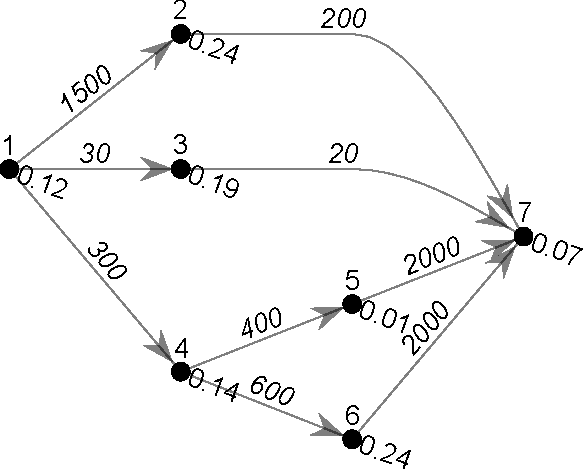
\includegraphics[width=\linewidth]{tcg1.pdf}
		\caption{}
		\label{fig:5a}
	\end{subfigure}\hspace{6mm}
	\begin{subfigure}{.2\textwidth}
		\centering
		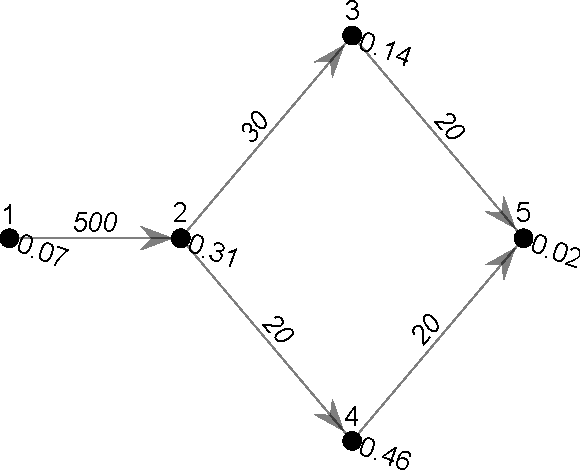
\includegraphics[width=\linewidth]{tcg2.pdf}
		\caption{}
		\label{fig:5b}
	\end{subfigure}
	
	\caption{Task call graph of a) WD1 and b) WD2. The numbers on each node represent the sequence in which the corresponding subtask is executed as well as the normalized computation cycle. Edge weights are input/output data sizes of subtasks in Kbits.} \label{fig:5}
\end{figure}

\begin{figure*}[ht]
	\centering
	\begin{subfigure}[b]{.22\textwidth}
		\centering
		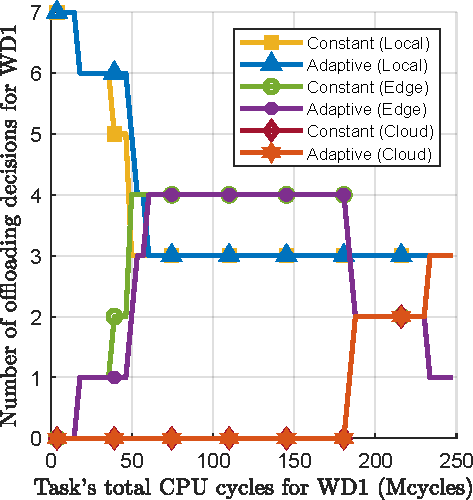
\includegraphics[width=\linewidth]{simulation_a.pdf}
		\caption{} \label{fig:6a}
	\end{subfigure}\hspace{15mm}
	\begin{subfigure}[b]{.22\textwidth}
		\centering
		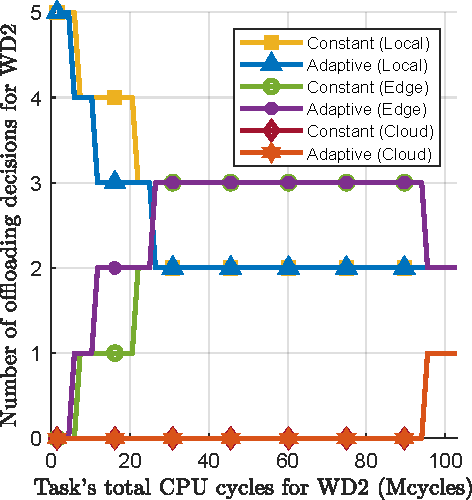
\includegraphics[width=\linewidth]{simulation_b.pdf}
		\caption{} \label{fig:6b}
	\end{subfigure}\hspace{15mm}
	\begin{subfigure}[b]{.22\textwidth}
		\centering
		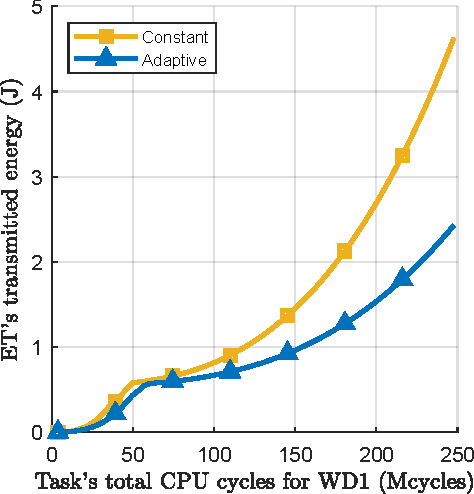
\includegraphics[width=\linewidth]{simulation_c.pdf}
		\caption{} \label{fig:6c}
	\end{subfigure}
	
	\caption{Impact of increasing the task's total number of CPU cycles \textcolor{blue}{(i.e., $\sum_{v_d\in\mathcal{V}_d}C_{v_d}$)} on a) The optimal number of offloading decisions of WD1, b) the optimal number of offloading decisions of WD2, and c) ET's transmitted energy, for constant and adaptive $\beta_{v_d^u}$ approaches.} \label{fig:6}
\end{figure*}

As the value of $U$ represents the maximum number of subtasks among devices, it does not scale with the size of network $D$. Therefore, we can consider it as a constant in analyzing time complexity. To summarize, by considering this fact, the depth and work of our parallel WiEnTM algorithm are $O(\log_2D)$ and $O(D)$, respectively.

\section{Performance Evaluation}
In this section, we investigate the performance of WiEnTM algorithm by evaluating the computation time of tasks and the ET's energy transmission. We further compare our proposed algorithm with an existing work in \cite{b13}.

\subsection{Simulation Setup}
We consider two devices WD1 and WD2 with task call graphs shown in Fig. \ref{fig:5a} and Fig. \ref{fig:5b}. \textcolor{blue}{These figures show the dependencies in the task call graph of each WD. An arrow leaving node $i$ toward $j$ indicates that task $j$ is dependent on task $i$.} The size of subtasks to be transferred between the devices and cloud/MEC server is shown in Kbits as the weight of edges. The normalized computation cycles of each subtask is also shown next to the vertices. This value reflects the required computation cycles for each subtask \textcolor{blue}{(i.e., $C_{v_d^u}, \forall d\in\mathcal{D}^u, \forall u\in\mathcal{U}$)} divided by the task's total computation cycle \textcolor{blue}{(i.e., $\sum_{u\in\mathcal{U}}C_{v_d^u}, \forall d\in\mathcal{D}$)}. Constant parameters are set as $\zeta_1=\zeta_2=10^{-28} \text{F}$ (i.e., CPU's effective switched capacitance)\cite{b2}, $\eta_1=\eta_2=0.51$ (i.e., energy harvesting efficiency) \cite{b2}, $\sigma^2=10^{-9}\text{W}$ (i.e., noise power) \cite{b2}, $\Gamma_1=0.8\text{s}$, $\Gamma_2=\Gamma_3=\Gamma_4=\Gamma_5=0.6\text{s}$, $\Gamma_6=0.3\text{s}$, $\Gamma_7=0.4\text{s} \text{ (i.e., length of each episode)}$, $P^{\text{ET}, \max} = 50\text{W}$, $P^{\text{AP}, \max} = 25\text{W}$, and $P^{\text{WD}, \max}_1 = P^{\text{WD}, \max}_2 = 25\text{mW}$. We set the cloud response times $\mu_{v_d^u}=20\text{ms}, \forall d\in\mathcal{D}^u, \forall u\in\mathcal{U}$ as inspired by \cite{b24}. We also set $B_1 = B_2 = 50\text{MHz}, F_{1}^{\text{L},\max} = F_{2}^{\text{L},\max} = 160\text{MHz}$, and $F^{\text{M},\max} = 2.2\text{GHz}$. We adopt the simplified path loss model \cite{b21} for wireless channel gains. Without loss of generality, we set $g_d = h_d = -5\text{dB}, \forall d\in\mathcal{D}$.

In order to analyze the effect of $\beta_{v_d^u}$ on the optimal solution, we consider two cases for $\beta_{v_d^u}$ :
1) Constant with $\beta_{v_d^u}=1, \forall v_d^u\in \mathcal{V}_d$, 2) adaptive $\beta_{v_d^u}$ with $0\leq k \leq 1$ given as follows.
\begin{equation}\label{eq32}
	\begin{aligned}
		\beta_{v_d^u} = &\frac{kC_{v_d^u}}{\sum_{d'\in\mathcal{D}^u}C_{v_{d'}^u}}|\mathcal{D}^u| +\\
		&\frac{(1-k)\sum_{v_d^i\in\mathcal{I}_{v_{d'}^u}}N_{v_{d'}^i,v_d^u}}{\sum_{d'\in\mathcal{D}^u}\sum_{v_{d'}^i\in\mathcal{I}_{v_{d'}^u}}N_{v_{d'}^i,v_{d'}^u}}|\mathcal{D}^u|,\quad\forall d\in\mathcal{D}^u, \forall u\in\mathcal{U},
	\end{aligned}
\end{equation}
where we consider $k=0.8$. Note that the above value is an example of adaptive $\beta_{v_d^u}$ and determining it's optimal value is beyond the scope of this work. \footnote{\textcolor{blue}{For the case of non-optimal $\beta_{v_d^u}$, one needs to analyze the approximation ratio of the proposed algorithm. An approach similar to \cite{b2} can be followed. However, we leave this extension as future work.}}

\begin{figure}
	\centering
	\begin{subfigure}[b]{.39\textwidth}
		\centering
		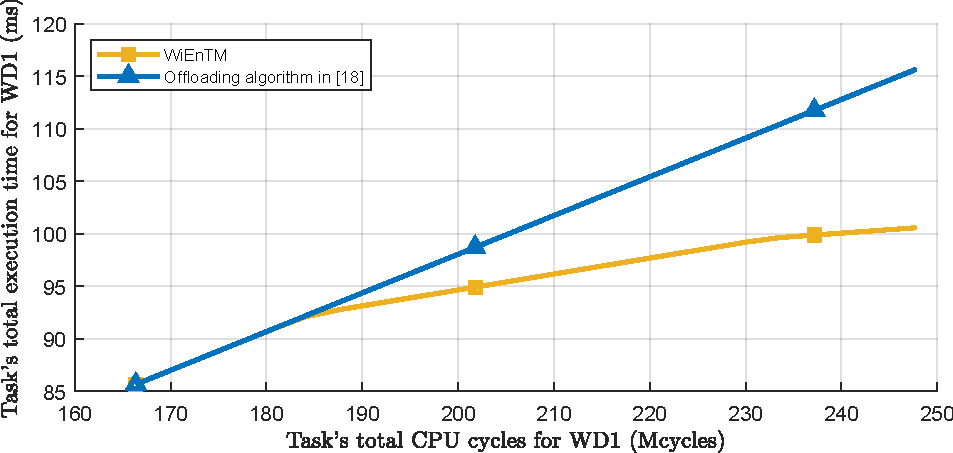
\includegraphics[width=\linewidth]{simulation2_a1.pdf}
		\caption{} \label{fig:7a1}
	\end{subfigure}
	\begin{subfigure}[b]{.39\textwidth}
		\centering
		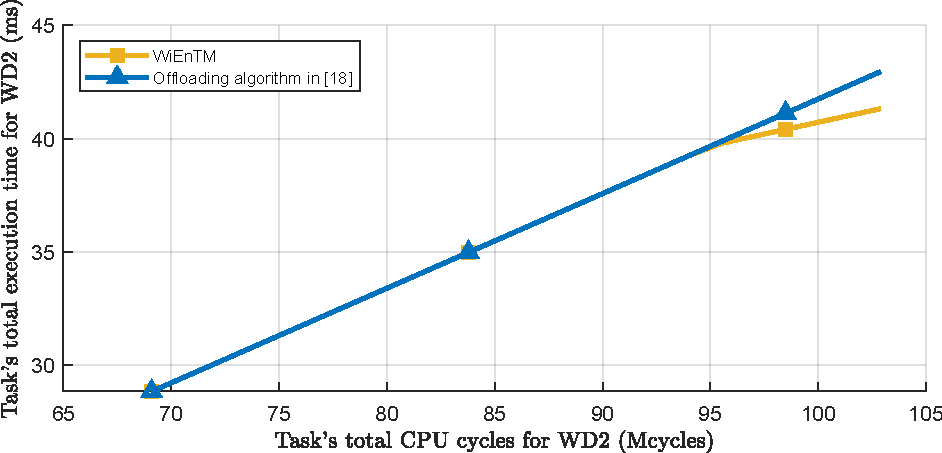
\includegraphics[width=\linewidth]{simulation2_b1.pdf}
		\caption{} \label{fig:7b1}
	\end{subfigure}
	
	\caption{The total computation time of our three-tier WPMEC and the scheme proposed in \cite{b13} for different task's total CPU cycles \textcolor{blue}{(i.e., $\sum_{v_d\in\mathcal{V}_d}C_{v_d}$)} for a) WD1, and b) WD2.} \label{fig:71}
\end{figure}

We now describe the intuition behind the adaptive $\beta_{v_d^u}$ value given in (\ref{eq32}). According to (\ref{eq2}) and (\ref{eq3}), it can be observed that increasing the number of CPU cycles and input/output data bits of each subtask will increase the energy required by the subtask. Constraint (\ref{eq28}) depicts that increasing $\beta_{v_d^u}$ will expand the feasible space for $\tau_{1,v_d^u}$ and $\tau_{2,v_d^u}$ which will decrease the energy consumption. Therefore, subtasks with high number of CPU cycles and high amount of input/output data bits are the bottleneck of energy consumption. As a result, modeling $\beta_{v_d^u}$ based on a weighted sum of normalized number of CPU cycles and input/output bits should decrease the energy consumption compared to assigning equal $\beta_{v_d^u}$ to all subtasks. 

\begin{figure}
	\centering
	\begin{subfigure}[b]{.37\textwidth}
		\centering
		\includegraphics[width=\linewidth]{simulation2_a.pdf}
		\caption{} \label{fig:7a}
	\end{subfigure}
	\begin{subfigure}[b]{.37\textwidth}
		\centering
		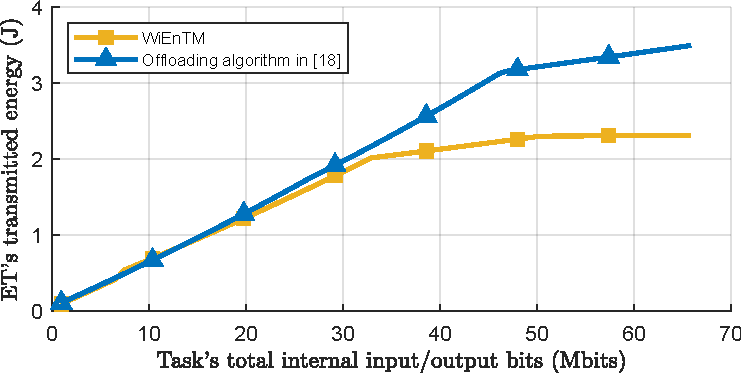
\includegraphics[width=\linewidth]{simulation2_b.pdf}
		\caption{} \label{fig:7b}
	\end{subfigure}
	
	\caption{\textcolor{blue}{Comparison of ET's transmitted energy between WiEnTM and the algorithm proposed in \cite{b13} for different a) task's CPU cycles (i.e., $\sum_{v_d\in\mathcal{V}_d}C_{v_d}$) and, b) task's internal input/output bits (i.e., $\sum_{v_d^i,v_d^j\in\mathcal{V}_d}N_{v_d^i,v_d^j}$).}} \label{fig:7}
\end{figure}

\subsection{Simulation Results}
Figs. \ref{fig:6a} and \ref{fig:6b} show the transition between different optimal offloading decisions as we increase the task's CPU cycles \textcolor{blue}{(i.e., $\sum_{u\in\mathcal{U}}C_{v_d^u}, \forall d\in\mathcal{D}$)} for WD1 and WD2, respectively. In both of these figures, we illustrate the number of offloading decisions for the local, edge, and cloud computing. Note that for each WD, the sum of offloading decisions is the number of subtasks. It can be observed that as we increase the task CPU cycles, the offloading decisions gradually transit from the local to the edge and finally to the cloud. Additionally, it is shown that for WD1 which has a larger number of task CPU cycles, the system relies more on the cloud server than WD2. Fig. \ref{fig:6c} shows the  optimal ET’s energy transmission. From Fig. \ref{fig:6c}, it can be perceived that adaptive technique offers up to 47\% less energy consumption in comparison with the constant $\beta_{v_d^u}$ approach. It means that setting $\beta_{v_d^u}$ according to the number of CPU cycles and input/output sizes greatly enhances the performance comparing to the constant approach.

By considering adaptive $\beta_{v_d^u}$ given in (\ref{eq32}), we also compare our proposed three-tier WPMEC system with the scheme proposed in \cite{b13}. Figs. \ref{fig:7a1} and \ref{fig:7b1} illustrate the task's execution time for WD1 and WD2, respectively. The results show that by using WiEnTM, up to $13\%$ overall less total computation time can be obtained for WD1 in comparison to \cite{b13}. This is because WD1 has a computationally intensive task. However, a lower improvement is achieved for WD2 as it has a lighter task which is mostly executed locally by the device or on the MEC server.

\textcolor{blue}{We further investigate the performance of our proposed WiEnTM algorithm by evaluating the ET's transmitted energy in comparison to that of \cite{b13}. Figs. \ref{fig:7a} and \ref{fig:7b} illustrate the effect of the task's CPU cycles and the task size (i.e., the number of input/output bits), respectively. The results show that by using WiEnTM, the ET consumes up to $34\%$ less energy compared to the algorithm in \cite{b13}.}

\textcolor{blue}{We now consider 200 WDs and investigate the ET transmission energy required to enable WDs execute their tasks. We study three different policies: 1) Local computing, 3) computation offloading, and 3) WiEnTM algorithm. We assume that among these devices, 100 WDs have a task with the call graph shown in Fig. \ref{fig:5a} and the rest with the task call graph of Fig. \ref{fig:5b}.} In the local computing case, all WDs harvest the energy to execute their subtasks locally while in the computation offloading case, the energy is used to offload all the subtasks. \textcolor{blue}{Fig. \ref{fig:9a} shows the ET's energy transmission when we vary the task's total CPU cycles. Additionally, Fig. \ref{fig:9b} illustrates the ET's energy for different numbers of the task's total input/output bits, which reflect the size of the tasks.} As can be observed, WiEnTM substantially reduces the required energy as it achieves the optimal offloading decisions. \textcolor{blue}{In particular, according to Fig. \ref{fig:9a}, comparing to the local computing case, a higher improvement is obtained for the computationally intensive tasks.} This is because the WDs require more energy to execute all their subtasks locally. However, for light tasks with low computation cycles, the WiEnTM algorithm significantly outperforms the offloading case as it is more preferred to execute such tasks locally. \textcolor{blue}{The results of Fig. \ref{fig:9b} imply that WiEnTM mainly follows the policy of offloading to edge/cloud server for tasks with a small number of input/output bits. As we increase the number of bits, the algorithm tends to rely more on local computing. As can be observed, WiEnTM greatly outperforms both schemes.} 

\begin{figure}
	\centering
	\begin{subfigure}[b]{.24\textwidth}
		\centering
		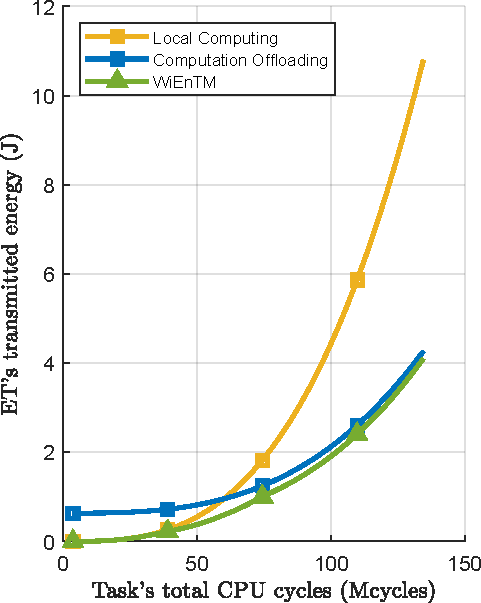
\includegraphics[height=1.2\linewidth]{simulation3_a.pdf}
		\caption{} \label{fig:9a}
	\end{subfigure}
	\begin{subfigure}[b]{.24\textwidth}
		\centering
		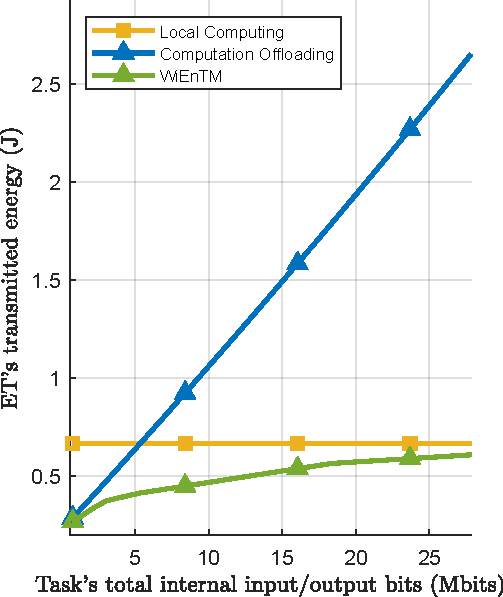
\includegraphics[height=1.2\linewidth]{simulation3_b.pdf}
		\caption{} \label{fig:9b}
	\end{subfigure}
	
	\caption{\textcolor{blue}{Comparison of ET's transmitted energy for three offloading policies when there are 200 WDs. 1) Local computation-only, 2) computation offloading-only, and 3) WiEnTM algorithm.}} \label{fig:9}
\end{figure}

\section{Conclusion}
In this paper, we studied a three-tier WPMEC system that is consisting of edge and cloud servers as well as WDs. We first proposed a harvest-then-offload mechanism that efficiently schedules the computing resources and allocates the wireless energy. This is achieved by formulating an optimization problem that aims to minimize the ET's energy transmission while satisfying the tasks computation deadline. We then proposed a matching algorithm called WiEnTM that optimally solves the aforementioned problem. We further proposed a parallel implementation of this algorithm with nearly logarithmic complexity. We also investigated the performance of WiEnTM through numerical experiments. Our results show a significant reduction in ET's transmitted energy compared to different offloading policies. \textcolor{blue}{Our algorithm also requires up to 34\% less overall ET's energy transmission compared to an existing work in the literature.}

For future work, we will consider the dynamic behavior of three-tier WPMEC system and propose an online learning approach to achieve the optimal decisions under uncertainty. \textcolor{blue}{We will also study more powerful WDs with full-duplex capability in future.}

\bibliographystyle{IEEEtran}
\bibliography{references}

\title{Responses to the Reviewers' Comments}

\maketitle

\vspace{-1.5cm}
\setstretch{1.6}

\setcounter{page}{1}

\begin{itemize}
	\item \textbf{Title of Manuscript}: A QoE-Oriented Computation Offloading Algorithm based on Deep Reinforcement Learning for Mobile Edge Computing
	
	
	\item \textbf{Authors}:  Iman Rahmati, Hamed Shah-Mansouri, and Ali Movaghar
	
	
	\item \textbf{Affiliation}: Departments of Electrical Engineering and Computer Engineering,  Sharif University of Technology, Tehran, Iran
	
	\item \textbf{Paper Reference Number}: TNSE-2024-03-0468 
	
\end{itemize}

\vspace{0.3cm}

\setstretch{1.2}

\noindent We would like to express our gratitude to the reviewers for their valuable recommendations toward improving the quality of our paper. We also want to gratefully thank the associate editor for handling the paper. Our responses to the reviewers' comments are given below. For convenience, we have used blue font for the revised or newly added paragraphs in the manuscript.\newline

\setcounter{section}{0}
\renewcommand*{\thesection}{\Roman{section}}
\makeatletter


\newpage

\section{Response to Reviewer 1}
\begin{enumerate}

\item \underline{Reviewer's Comment}: 
\textit{``Lots of the studies focus on the research on resource optimisation of MEC by DRL, it is expected to survey the state-of-the-art within 3 years, and summarise it as an individual section, departing from the Section of Introduction. Besides, the existing related work only has one paragraph without any discussion about the pros/cons of the previous work.''} \newline

\underline{Authors' Reply}:\\

Ref

\item \underline{Reviewer's Comment}: 
\textit{``Please highlight what and how the proposed approach provides "high performance" to further specify the motivations and contributions. Especially, please highlight the reason why the authors design the framework by integrating LSTM. Otherwise, it will make the innovations seem weak.''} \newline

\underline{Authors' Reply}:\\

\item \underline{Reviewer's Comment}: 
\textit{``In section III, why is the size of the task selected from a discrete set? Is it selected randomly or in another way? Besides, the authors define the offloading indicate function as $y_{i,j}(t$, it should be involved when modelling the Edge Execution phrase.''} \newline

\underline{Authors' Reply}:\\

\item \underline{Reviewer's Comment}: 
\textit{``Some sota methods (e.g., DDQN, DDPG) are expected to be compared in the section on performance evaluation, and authors should have more discussions about the evaluation results rather than merely introducing them. Besides, I think it is better to design the evaluations with a real dataset. Besides, 9\% and 6\% are not significant improvements compared to other methods.''} \newline

\underline{Authors' Reply}:\\

\item \underline{Reviewer's Comment}: 
\textit{``Other concerns are also expected to be addressed: (a) be careful to use words like "battery level" to express the energy consumption, because some of the energy is provided by the wired line power. (b) Most of the references are out of 3 years, please investigate more studies published in recent years. (c) The authors should thoroughly check the writing style, grammar, and spelling to enhance the paper's clarity, conciseness, and overall impact.''} \newline

\underline{Authors' Reply}:\\

Ref

\end{enumerate}


\newpage

\section{Response to Reviewer 2}
\begin{enumerate}
	
	\item \underline{Reviewer's Comment}: 
	\textit{``The authors should provide a comparative table to highlight their contributions. Specially, the authors should compare their method with other references on computation task offloading cited in the paper, including aspects such as scenarios, methods, advances, drawbacks, and so on.''} \newline
	
	
	\underline{Authors' Reply}:\\
	Ref
	
	\begin{table*}[htbp]\textcolor{blue}{
			\renewcommand{\arraystretch}{0.7}
			\captionsetup{name=TABLE}
			\caption{Comparison of Related Works}
			\scalebox{0.7}{%
				\begin{tabular}{ lp{2.3cm}p{4.5cm}p{5cm}p{1.5cm}p{3cm}p{5cm}l} 
					\toprule
					\textbf{Paper} & \textbf{Scenario} &  \textbf{Problem} &  \textbf{Objective} &  \textbf{Model} & \textbf{Algorithm/Methods} &  \textbf{Drawbacks}  \\ \midrule
					\cite{huang2019deep} & Wireless-powered MEC & Computation offloading and resource allocations & Maximize computation rate & MIP & DQN & Not consider delay-sensitive tasks \\\midrule
					\cite{Bolourian-WCL24} & MEC with EH devices& Energy harvesting  computation offloading & Minimize drop rate and energy consumption. & MDP  & Deep Q-Learning & \\\midrule
					\cite{zhao2019deep} & MEC & Wireless channels competition & Optimize downlink utility & MDP & Multi-agent D3QN & \\\midrule
					\cite{9253665} &  MEC &  Computation offloading & Minimize drop rate and computation delay. & MDP & D3QN + LSTM & Not consider system energy consumtion\\\midrule
					\cite{sun2024hierarchical} & MEC & Computation offloading and service caching & Minimize average service delay & MDP & hierarchical DRL & Not consider system energy consumtion \\\midrule
					\cite{dai2020edge} & MEC & Resource allocation and computation offloading & Minimize energy consumption & MDP & DDPG & \\\midrule
					\cite{huang2021deadline} & MEC & Computation offloading & Minimizing total energy consumption & POMDP & DDPG & \\ \midrule
					\cite{liu2021learn} & MEC & Resource allocation and computation offloading & Minimize execution cost & POMDP & MADRL &  Not consider delay-sensitive tasks \\\midrule
					\cite{zhou2021deep} & MEC & Resource allocation and computation offloading & Minimize energy consumption of the entire system & MDP & DDQN & Only for a singel MEC system model \\\midrule
					\cite{gao2022large} & heterogeneous MEC & Decentralized computation offloading & Optimize system cost and completion rates & MDP & Multi-agent DDPG & Not take MD's demans into consideration \\\midrule
					\cite{gong2022edge} & MEC-based IIoT & Resource allocation and computation offloading & Minimize task computation delay and energy consumption & MDP & DRL & Not take MD's demans into consideration\\\midrule
					\cite{liao2023online} & MEC & Online computation offloading & Minimize computation delay and energy consumption & MDP & DDQN & Only for a singel MEC system model  \\\midrule
					\cite{wu2023multi} & MEC-based IIoT & Computation offloading & Optimize delay and energy consumption & POMDP & Multi-agent DQN& \\\midrule
					\cite{wu2023computation} & SDN-based MEC & Stochastic game-based resource allocation & Minimize energy consumption and processing delay & MDP & MARL & \\\midrule
					\cite{wu2024privacy} & MEC-based IIoT  & Joint power allocation and computation offloading  & Optimization of privacy protection and quality of service. & MDP & Multi-agent DDPG & \\\midrule
					\cite{wu2024combining} & MEC-based IIoT & Privacy aware computation offloading & Optimization of computation rate and energy consumption & MDP & DDPG  & \\\midrule
					QECO &  MEC &  Computation offloading & Maximize the QoE of each MD individually &MDP & D3QN + LSTM & \\
					\toprule
			\end{tabular}}
			\label{table}}
	\end{table*}
	
	
	\newpage
	\item \underline{Reviewer's Comment}: 
	\textit{``I think more explanations should be added for the QoE function. How can the defined function reflect QoE?''} \newline
	
	\underline{Authors' Reply}:\\
	\newpage
	\item \underline{Reviewer's Comment}: 
	\textit{``(a) What inputs and outputs of Algorithm 2? (b) They should be added to make readers clearly understand the results.''} \\\newline
	\underline{Authors' Reply}: (a) To address the reviewer concern about algorithm 2, we have revised secound paragraph of subsection (Training Process Algorithm at EN $j \in \mathcal{J})$ in Section IV to clarify the inputs and outputs of algorithms 2, as follows. \newline
	
	\begin{my}{1cm}{1cm}
		\rev{In particular, regarding experience $n$, the target-Q value $\hat{Q}_{i,n}^{\text{T}}$ represents the long-term QoE for action $\boldsymbol{a}_i(n)$ under state $\boldsymbol{s}_i(n)$. This value corresponds to the QoE observed in experience $n$, as well as the approximate expected upcoming QoE. 
			\textcolor{blue}{Based on the previous sample experiences $\mathcal{N}$, the EN computes the vector $\hat{\mathbf{Q}}_i^{\text{T}} = (\hat{Q}^{\text{T}}_{i,n})_{n \in \mathcal{N}}$ and trains the MD's neural network (in steps 11-21 of Algorithm ~\ref{alg:cap2}) to keep parameter vector $\theta^{\text{E}}_i$ in $\textit{Net}_i^{\text{E}}$ update for the MD's \textit{UpdateRequest}}. The key idea of updating $\textit{Net}_i^{\text{E}}$ is to minimize the disparity in Q-values between $\textit{Net}_i^{\text{E}}$ and $\textit{Net}_i^{\text{T}}$, as indicated by the following loss function:\\ \dots}
	\end{my}
		
	We have also revised algorithm 1 and 2, as below.\\	
	

\begin{my}{0.5cm}{0.5cm}	
\rev{\begin{minipage}[b]{0.87\textwidth} 
	\begin{algorithm}[H] \caption{QECO Algorithm (Training Process)}\label{alg:cap2} \centering 
		\begin{algorithmic}[1] \renewcommand{\algorithmicrequire}{\textbf{\textcolor{blue}{Input:}}} \renewcommand{\algorithmicensure}{\textbf{\textcolor{blue}{Output:}}} \Require \textcolor{blue}{experience $(\boldsymbol{s}_i(t), \boldsymbol{a}_i(t), \boldsymbol{q}_i(t), \boldsymbol{s}_i(t+1))$ from MD $i \in \mathcal{I}$} \Ensure \textcolor{blue}{parameter vector $\theta_i^{\text{E}}$} 
	\end{algorithmic} 
\end{algorithm} 
\end{minipage}
\vspace{5mm}

\begin{minipage}[b]{0.87\textwidth} 
	\begin{algorithm}[H] \caption{QECO Algorithm (Offloading Decision)}\label{alg:cap2} \centering 
		\begin{algorithmic}[1] \renewcommand{\algorithmicrequire}{\textbf{Input:}} \renewcommand{\algorithmicensure}{\textbf{Output:}}\Require state space $\mathcal{S}$, action space $\mathcal{A}$
			\Ensure MD $i \in \mathcal{I}$ experience  \textcolor{blue}{ $(\hspace{-0.2mm}\boldsymbol{s}_i(\hspace{-0.2mm}t\hspace{-0.2mm}), \boldsymbol{a}_i(\hspace{-0.2mm}t\hspace{-0.2mm}), \boldsymbol{q}_i(\hspace{-0.2mm}t\hspace{-0.2mm}), \boldsymbol{s}_i(\hspace{-0.2mm}t\hspace{-0.3mm}+\hspace{-0.3mm}\hspace{-0.2mm}1\hspace{-0.2mm}\hspace{-0.2mm})\hspace{-0.2mm})$}
		\end{algorithmic} 
	\end{algorithm} 
\end{minipage}}
\end{my}
	

\vspace{10mm}
	\item \underline{Reviewer's Comment}: 
	\textit{``The authors should open their experiments in github, so that other researchers can compare their work with other ones.''} \newline
	\underline{Authors' Reply}: To address the reviewer comment, we make our experiments more accessible by sharing our GitHub rerepository. We have added it into the end of first paragraph of Section V, as follows.
	\begin{my}{1cm}{1cm}
		\rev{Detailed settings regarding the neural networks and simulation can be found at our github repository. }
	\end{my}
	We have also provided repository URL link in the footnote of Page 8 as below.
	\begin{my}{1cm}{1cm}
		\rev{The code for reproducing the simulation results of this letter is available at\newline https://github.com/ImanRHT/QECO.} \newline
	\end{my}

\newpage
	\item \underline{Reviewer's Comment}: 
	\textit{``The following references closely related to the current work should be discussed or compared with the current work for completeness.''} \newline
		\begin{my}{1cm}{1cm}
		\rev{
			{\small
				\noindent\cite{b35} G. Wu, Z. Xu, H. Zhang, S. Shen, and S. Yu,  ``Multi-agent DRL for joint completion delay and energy consumption with queuing theory in MEC-based IIoT,'' in \textit{Journal of Parallel and Distributed Computing}, vol. 176, pp. 80–94, Jun. 2023.\\[6pt]
				\cite{b38} G. Wu, H. Wang, H. Zhang, Y. Zhao, S. Yu, and S. Shen, ``Computation offloading method using stochastic games for software-defined-network-based multiagent mobile edge computing,'' \textit{IEEE Internet of Things Journal}, vol. 10, no. 20, pp. 17620–17634, Oct. 2023.\\[6pt]
				\cite{b37} G. Wu, X. Chen, Z. Gao, H. Zhang, S. Yu, and S. Shen, ``Privacy-preserving offloading scheme in multi-access mobile edge computing based on MADRL,'' \textit{Journal of Parallel and Distributed Computing}, vol. 10, no. 1, pp. 451--460, Mar. 2022.\\[6pt]
				\cite{b39} G. Wu, X. Chen, Y. Shen, Z. Xu, H. Zhang, S. Shen, and S. Yu,``Combining Lyapunov optimization with Actor-Critic networks for privacy-aware IIoT computation offloading,'' in \textit{IEEE Internet of Things Journal}, 2024, Early Access\\[10pt]}\\}
	\end{my}

	
	\underline{Authors' Reply}:\\
	
	We have also cited these works in the following sentences in Section I of the revised manuscript.\\

\begin{my}{1cm}{1cm}
	\rev{
		
		
		$\cdots$
		
	
		}
\end{my}
	
\end{enumerate}

\newpage

\section{Response to Reviewer 1}
\begin{enumerate}
	
	\item \underline{Reviewer's Comment}: \textit{``(a) The Introduction is verbose and confusing. (b) The authors should consider clarifying the relationship between task offloading and energy optimization in this paper.''} \newline

\underline{Authors' Reply}: (a) To address the reviewer comment, we have first summarized the explanation of the Internet of Things (IoT) applications, mobile edge computing (MEC), and the motivations of the proposed three-tier computing model. We have revised the first paragraph of Section I as follows.\\

\begin{my}{1cm}{1cm}
	\rev{The Internet of Things (IoT) applications (e.g., smart cities \cite{b1}, homes \cite{b3}, and augmented/virtual reality \cite{b11}) are mostly involved with computation-intensive and latency-sensitive tasks. Mobile edge computing (MEC) is a state-of-the-art computation paradigm to address the challenge of insufficient computing resources in IoT networks \cite{b35, b4}. By deploying the edge servers, nearby devices can offload their computation tasks. Dispatching those tasks that require a higher amount of energy will let devices save more energy \cite{b38}. However, as the computation tasks become more and more intensive, coordination with cloud servers will be inevitable \cite{b37}. The three-tier computing models consisting of cloud, edge, and IoT devices are introduced to overcome the aforementioned challenge \cite{b5,b6,b39,b40}. }\newline
\end{my}

We have also revised the second paragraph of Section I to better emphasize the role of the proposed system in overcoming the challenges of IoT systems.\\	

\begin{my}{1cm}{1cm}
	\rev{In addition to their restricted computation resources, IoT devices usually have small battery capacities which is mainly due to their small form factor and the constraints of the production cost \cite{b1}.
	
	$\cdots$
	
By combining the advantages of MEC and WPC, the newly emerged wireless powered MEC (WPMEC) holds a major promise to overcome the fundamental hurdles in scalability of the IoT networks \cite{b9,b10,b30,b33}.}\newline
	
\end{my}

(b) Furthermore, we clarify the relationship between computation offloading and energy optimization. Note that in WPMEC systems, the energy for the operation of WDs is provided by the HAP. Thus, we formulate an optimization problem to minimize the total energy consumption of the HAP at the ET by jointly considering computation offloading, scheduling, and power allocation while guaranteeing the task completion and energy constraints. The following explanations have been added to Section I of the revised manuscript. \\

\begin{my}{1cm}{1cm}
	\rev{ 
		By deploying the edge servers, nearby devices can offload their computation tasks. Dispatching those tasks that require a higher amount of energy will let devices save more energy \cite{b38}.
		
		$\cdots$
		
However, due to the limitation of WET and the cost of ETs, reducing the energy consumption is crucial.

$\cdots$		
		
It helps WDs save more energy and reduce the tasks' execution time, which consequently reduces the energy consumption of WPMEC system as WDs harvest energy from ETs.}\newline
	
\end{my}

We have also revised the first paragraph of Section III.A to address the reviewer comment. \\

\begin{my}{1cm}{1cm}
	\rev{In WPMEC systems, the energy for the operation of WDs is provided by the HAP.  Due to the high attenuation of WET over distances \cite{b8}, a considerable amount of energy is required to be provided for sustainable operation of WDs, which imposes a high cost to HAP. In this paper, we formulate an optimization problem to minimize the total energy consumption of the HAP at the ET by jointly considering computation offloading, scheduling, and power allocation while guaranteeing the task completion and energy constraints.} \newline
\end{my} 

We hope the above changes make the introduction more concise and less confusing.\\

\item \underline{Reviewer's Comment}: \textit {``The authors introduce many works on computation offloading and energy consumption, however, the contributions of the paper are not clear.''} \newline

\underline{Authors' Reply}: We first clarify our contributions in comparison to the existing works. In the ETEM problem formulation, unlike other works in the WPMEC literature (e.g., \cite{b11,b13,b28}), we first consider a three-tier computing paradigm that includes wireless devices, edge servers, and the remote cloud server. This architecture helps in further scaling WPMEC systems in terms of computation capability. We also take the MEC server computation time into account to more accurately model the MEC servers. Another main contribution is considering task interdependencies to capture real-world applications. In the WiEnTM algorithm, we first exploit the bipartite graph matching to tackle the complexity of the combinatorial ETEM problem. With efficient parallelization, we then propose a low complexity algorithm that can solve ETEM in real-time.

In summary, the main contributions of our work are:

\begin{enumerate}
	\item Formulating ETEM problem for a three-tier wireless powered mobile edge computing system considering task interdependencies and MEC server computation time to minimize the energy consumption.
	\item Proposing WiEnTM offloading and scheduling algorithm that greatly enhances energy efficiency while imposing a logarithmic time complexity by leveraging parallel processing and bipartite graph matching. Therefore, the algorithm can easily accommodate the real-time requirements of an offloading scheme. In order to apply the matching algorithm to ETEM problem, we study the characteristics of the problem. We first reduce it into a simplified form (i.e., S-ETEM). Next, we introduce a design parameter $\beta_{v_d^u}$ for each subtask $v_d^u\in\mathcal{V}_d$ of WD $\mathcal{D}^u$ and episode $u\in\mathcal{U}$ to decompose it into a number of independent problems (i.e., DS-ETEM).
	\item Evaluating the performance of WiEnTM in different scenarios and comparing to other state-of-the-art algorithms.
\end{enumerate}

In Section I of the revised manuscript, we have further explained the related works and clarified our main contributions as follows.\\

\begin{my}{1cm}{1cm}
	\rev{
		\textcolor{blue}{In \cite{b39}, authors proposed a scheme that aims to minimize the total cost in terms of energy and delay for a three-tier cloud-edge-IoT system. Gao \textit{et al.} in \cite{b40} proposed an offloading algorithm to minimize an objective called the energy time cost for a three-tier network. Although \cite{b5}, \cite{b39}, and \cite{b40} all benefit from a computationally-scalable three-tier system, IoT devices still rely on battery energy and hence lack the sustainability feature of WPMEC systems.}
		
		$\cdots$
		
		However, the proposed system model is oversimplified and thus less applicable to real-world scenarios.\\
	}
\end{my}

To make the contributions more clear, we have made the following changes to Section I of the revised manuscript.\\

\begin{my}{1cm}{1cm}
	\rev{\textcolor{blue}{By considering the challenges of the aforementioned works, the following questions arise:}
\begin{enumerate}
	\item \textcolor{blue}{\textit{How can we take advantage of cloud computing in addition to MEC to meet different requirements of IoT applications?}}
	\item \textcolor{blue}{\textit{How can we provide RF energy to enable the battery-less IoT devices operate seamlessly?}}
	\item \textcolor{blue}{\textit{What would be the optimal offloading decision when considering the subtasks' interdependencies?}}
\end{enumerate}
	
$\cdots$	
	
	
	
		\begin{enumerate}
			\item \textcolor{blue}{\textit{Problem formulation}: We formally define the mixed-integer ET's energy minimization (ETEM) problem by deciding on offloading, WET time, and computation scheduling of subtasks for a multi-user three-tier WPMEC system} considering task interdependencies and MEC server computation time.
			\item \textcolor{blue}{\textit{Algorithm design}: We propose wireless energy transmission minimization (WiEnTM) algorithm based on bipartite graph matching. We first study the properties of the problem to decompose it into individual problems for each subtask to make it suitable for the matching algorithm.} By efficiently utilizing parallel processing on decomposed problems, we prove that our proposed algorithm has a logarithmic time complexity with respect to the network size.
			\item \textcolor{blue}{\textit{Performance evaluation}: Extensive numerical experiments are carried out to evaluate the proposed algorithm. Our experiments show major reduction in the WDs' required energy in comparison with baseline offloading policies.} The algorithm also reduces the energy consumption by 34\% for large tasks compared to an existing work \cite{b13}.\\
		\end{enumerate}
	}
\end{my}

\item \underline{Reviewer's Comment}: \textit {``Experiments need to be improved. WiEnTm proposed by this paper only compares time with WPMEC- [16]. However, WiEnTm is an energy optimization algorithm, and the main purpose of this paper is energy efficiency. I would like to know the energy performance of WiEnTm compared to other works, but it is not reflected in the paper. In addition, if authors want to show the performance of the proposed mechanism in various aspects, then it is necessary to compare it with state-of-the-art works.''} \newline

\underline{Authors' Reply}: To address the reviewer's comment, we have included Fig. \ref{fig:7r} in Section V of the revised manuscript. This figure shows the energy consumption of our proposed algorithm in comparison to a state-of-the-art work in the literature. We have also updated the following paragraph in Section V of the revised manuscript to explain the results.\newline
\begin{my}{1cm}{1cm}
	\rev{We further investigate the performance of our proposed WiEnTM algorithm by evaluating the ET's transmitted energy in comparison to that of \cite{b13}. Figs. \ref{fig:7ar} and \ref{fig:7br} illustrate the effect of the task's CPU cycles and the task size (i.e., the number of input/output bits), respectively. The results show that by using WiEnTM, the ET consumes up to $34\%$ less energy compared to the algorithm in \cite{b13}.\\
	}

\end{my}

\setcounter{figure}{7}
\begin{figure}
	\centering
	\begin{subfigure}[b]{.43\textwidth}
		\centering
		\includegraphics[width=\linewidth]{simulation2_a.pdf}
		\caption{} \label{fig:7ar}
	\end{subfigure}
	\begin{subfigure}[b]{.43\textwidth}
		\centering
		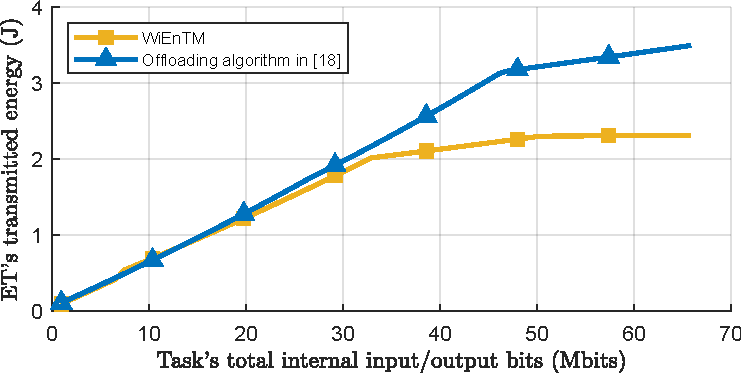
\includegraphics[width=\linewidth]{simulation2_b.pdf}
		\caption{} \label{fig:7br}
	\end{subfigure}
	
	\caption{\textcolor{blue}{Comparison of ET's transmitted energy between WiEnTM and the algorithm proposed in \cite{b13} for different a) task's CPU cycles (i.e., $\sum_{v_d\in\mathcal{V}_d}C_{v_d}$) and, b) task's internal input/output bits (i.e., $\sum_{v_d^i,v_d^j\in\mathcal{V}_d}N_{v_d^i,v_d^j}$).}} \label{fig:7r}
\end{figure}

 \setstretch{1.2}

\end{enumerate}

We highly appreciate the reviewer for the comments and suggestions. We hope that we have properly addressed these issues.


\section{Response to Reviewer 2}
\begin{enumerate}


\item \underline{Reviewer's Comment}: \textit{``It would be great if the authors provided one or multiple tables of key symbols and their corresponding description in the appendix or paper body instead of describing them in the text. This way is much easier to refer to the symbols.''} \newline

\underline{Authors' Reply}: In the revised manuscript, we have added the following table which includes the key notations alongside their descriptions. 

\setcounter{table}{0}

\begin{my}{0cm}{0cm}
	\rev{
		\begin{table}[h]
			\centering
			\caption{\textcolor{blue}{List of key notations}}
			\label{table2}
			{\color{blue}\begin{tabular}{ |p{2cm}|p{12cm}|  }
				\hline
				\textbf{Symbol} & \textbf{Description} \\
				\hline
				$x^{\text{L}}_{v_d^u}, x^{\text{M}}_{v_d^u}, x^{\text{C}}_{v_d^u}$ & Binary offloading decisions \\
				$\tau_{1,v_d^u}$ & Length of scheduled time for data transmission of subtask $v_d^u$ \\
				$\tau_{2,v_d^u}$ & Length of scheduled time for execution of subtask $v_d^u$\\
				$\tau_{3,v_d^u}$ & Length of scheduled time for retrieving the result of subtask $v_d^u$ \\
				$\tau_0^u$ & WET time in episode $u$\\
				$p^{u}$ & ET's power in episode $u$ \\
				$\Gamma^u$ & Length of episode $u$ \\
				$\mu_{v_d^u}$ & Response time of cloud server for subtask $v_d^u$ \\
				$C_{v_d^u}$ & Number of CPU cycles required for subtask $v_d^u$ \\
				$N_{i,j}$ & Number of bits required to transmit the result of subtask $i$ and $j$ \\
				$g_d$ & Channel gain between WD $d$ and ET \\
				$h_d$ & Channel gain between WD $d$ and MEC server \\
				$\sigma^2$ & Noise power at the HAP \\
				$\eta_d$ & Energy harvesting efficiency of WD $d$ \\
				$\zeta_{d}$ & CPU's effective switched capacitance of WD $d$ \\
				$r_{t,v_d^u}$ & Virtual resource for tier $t$ and subtask $v_d^u$ \\
				$F^{\text{M},\max}$ & Maximum CPU frequency of MEC server \\
				$F^{\text{L},\max}_{d}$ & Maximum CPU frequency of WD $d$ \\
				$P^{\text{ET},\max}$ & ET's maximum transmission power \\
				$P^{\text{AP},\max}$ & AP's maximum transmission power \\
				$P^{\text{WD},\max}_d$ & Maximum transmission power of WD $d$ \\
				$D$ & Number of WDs \\
				$V_d$ & Number of subtasks of WD $d$ \\
				$B_d$ & Bandwidth of WD $d$ \\
				$\mathcal{D}$, $\mathcal{D}^u$ & Set of WDs \\ 
				$\mathcal{U}$ & Set of episodes \\
				$\mathcal{V}_d$ & Set of subtasks of WD $d$ \\
				$\mathcal{R}^{\text{virt}}$ & Set of virtual resources \\
				$\mathcal{I}_{v_d^u}$ & Set of episodes associated to executing prerequisite subtasks of the subtask $v_d^u$ \\
				$\mathcal{J}_{v_d^u}$ & Set of episodes associated to executing subtasks with the subtask $v_d^u$ as their prerequisite \\
				\hline
			\end{tabular}}
	\end{table}}
\end{my}

 \setstretch{1.2}

\end{enumerate}

We would like to gratefully thank the reviewer for the valuable suggestion and comment. We hope that we have addressed this comment satisfactorily. \newpage

\section{Response to Reviewer 3}
\begin{enumerate}

\item \underline{Reviewer's Comment}: \textit{``Although the optimization objective of the investigated problem is to minimize energy consumption of the HAP, the time consumption for all subtasks generated by WDs still should be constrained. Otherwise, the QoS of latency-sensitive tasks cannot be guaranteed by the proposed algorithms.''} \newline

\underline{Authors' Reply}: The time consumption for all subtasks generated by WDs are indeed constrained in our work. With the introduction of episodes, we have simultaneously addressed the requirements of harvest-then-offload mechanism and the subtasks' deadlines. Constraint (\ref{eq9}) applies a hard deadline $\Gamma^u$ on each episode $u\in\mathcal{U}$ (i.e., a cycle of subtasks' executions) which is obtained based on the deadline of subtasks. In order to clarify this, we have included the following sentences in Section III of the revised manuscript. \newline

\begin{my}{1cm}{1cm}
\rev{	
	It is worth noting that inequality (\ref{eq9}) also enforces a hard deadline for each cycle of subtasks' execution in each episode. Thus, the total execution time of each task generated by WDs is constrained. This way, we can address the requirements of latency-sensitive tasks as well.
}\newline
\end{my}

Furthermore, we have included the following sentences to better illustrate the intention behind defining an \textit{episode} in Section II of the revised manuscript.\\

\begin{my}{1cm}{1cm}
	\rev{We regard a complete cycle of executing a single subtask for all WDs having a candidate subtask as an \textit{episode}. Each episode jointly models the harvest-then-offload timing, subtasks' deadlines, and TDMA scheduling of WDs.
	}\newline
\end{my}

\item \underline{Reviewer's Comment}: \textit {``(a) The definition of an “episode” is not stated clearly. (b) The first question is how to decide the length of an episode? (c) Since the length of an episode will affect the performance of scheduling, it should be analyzed theoretically. (d) Besides, how to decide the number of episodes?''} \newline

\underline{Authors' Reply}: We address each of the above comments one by one.\newline

(a) In Section II of the revised manuscript, we have first clarified the definition of an episode as follows.\\

\begin{my}{1cm}{1cm}
\rev{We regard a complete cycle of executing a single subtask for all
	WDs having a candidate subtask as an \textit{episode}. Each episode
	jointly models the harvest-then-offload timing, subtasks' deadlines, and TDMA scheduling of WDs.}\newline

\end{my}

(b) An episode is a complete cycle of subtasks' execution, including harvest-then-offload timing and subtasks' deadlines. Therefore, similar to other works in the literature of WPMEC (e.g., \cite{b2,b13,b28}), we consider that the length of an episode is directly related to subtasks' deadlines. In the revised manuscript, we have included the following paragraph in Section II to discuss an approach to calculate the length of an episode.\newline

\begin{my}{1cm}{1cm}
	\rev{Now that we have introduced the network model, we need to provide an approach to calculate the length of episode $\Gamma$. As stated earlier, each episode reflects the requirements of the harvest-then-offload timing and subtask deadlines. Therefore, $\Gamma$ is directly related to the individual subtask deadlines being executed in that episode. In other words, $\Gamma$ can be calculated as the summation of the subtasks' deadlines. In the next section, we will calculate the length of each episode.}\newline
	
\end{my}

(c) The length of an episode is present in inequality constraint (\ref{eq9}). Thus, a longer episode (i.e., the subtasks' deadlines) will enlarge the feasible region of the ETEM optimization problem and enhances the optimal solution and results in less energy consumption. In Section V, we have used this intuition to propose the adaptive approach for calculating the $\beta_{v_d^u}$ parameters. To further clarify, we have included the following sentences in Section III of the revised manuscript.\newline

\begin{my}{1cm}{1cm}
	\rev{Also, it can be concluded that $\Gamma^u$ is a key factor in the optimal value of the ETEM problem. A longer episode (i.e., larger $\Gamma^u$) provides more time for execution of the tasks. In fact, this will enlarge the feasible region of the ETEM optimization problem and enhances the energy-efficiency of the algorithm.}\newline
\end{my}

(d) The number of episodes corresponds to the time horizon of the problem. We defined the horizon to be the time required to accomplish a task on all WDs. Therefore, as long as there exists a subtask to be executed on WDs, a new episode will be required. This will result in having $\max_{d\in\mathcal{D}}V_d$ episodes. In the revised manuscript, we have updated the following sentences to further clarify how the number of required episodes (i.e., $U$) is calculated.\\

\begin{my}{1cm}{1cm}
	\rev{We denote $\mathcal{U}\triangleq\{0,...,U-1\}$ as the set of episodes, where $U\triangleq\max_{d\in\mathcal{D}}V_d$  indicates the number of episodes. Note that $V_d$ is obtained from the call graph of the corresponding task. \newline}
\end{my}

\item \underline{Reviewer's Comment}: \textit {``There are too many symbols in this paper. It is hard for readers to quickly find the meaning of each symbol. A symbol table should be added to improve the readability of this paper.''} \newline

\underline{Authors' Reply}: In the revised manuscript, we have added Table \ref{table3} which includes the key notations alongside their descriptions. \newline

\setcounter{table}{0}

\begin{my}{1cm}{1cm}
	\rev{		\begin{table}[h]
			\centering
			\caption{\textcolor{blue}{List of key notations}}
			\label{table3}
			{\color{blue}\begin{tabular}{ |p{2cm}|p{12cm}|  }
				\hline
				\textbf{Symbol} & \textbf{Description} \\
				\hline
				$x^{\text{L}}_{v_d^u}, x^{\text{M}}_{v_d^u}, x^{\text{C}}_{v_d^u}$ & Binary offloading decisions \\
				$\tau_{1,v_d^u}$ & Length of scheduled time for data transmission of subtask $v_d^u$ \\
				$\tau_{2,v_d^u}$ & Length of scheduled time for execution of subtask $v_d^u$\\
				$\tau_{3,v_d^u}$ & Length of scheduled time for retrieving the result of subtask $v_d^u$ \\
				$\tau_0^u$ & WET time in episode $u$\\
				$p^{u}$ & ET's power in episode $u$ \\
				$\Gamma^u$ & Length of episode $u$ \\
				$\mu_{v_d^u}$ & Response time of cloud server for subtask $v_d^u$ \\
				$C_{v_d^u}$ & Number of CPU cycles required for subtask $v_d^u$ \\
				$N_{i,j}$ & Number of bits required to transmit the result of subtask $i$ and $j$ \\
				$g_d$ & Channel gain between WD $d$ and ET \\
				$h_d$ & Channel gain between WD $d$ and MEC server \\
				$\sigma^2$ & Noise power at the HAP \\
				$\eta_d$ & Energy harvesting efficiency of WD $d$ \\
				$\zeta_{d}$ & CPU's effective switched capacitance of WD $d$ \\
				$r_{t,v_d^u}$ & Virtual resource for tier $t$ and subtask $v_d^u$ \\
				$F^{\text{M},\max}$ & Maximum CPU frequency of MEC server \\
				$F^{\text{L},\max}_{d}$ & Maximum CPU frequency of WD $d$ \\
				$P^{\text{ET},\max}$ & ET's maximum transmission power \\
				$P^{\text{AP},\max}$ & AP's maximum transmission power \\
				$P^{\text{WD},\max}_d$ & Maximum transmission power of WD $d$ \\
				$D$ & Number of WDs \\
				$V_d$ & Number of subtasks of WD $d$ \\
				$B_d$ & Bandwidth of WD $d$ \\
				$\mathcal{D}$, $\mathcal{D}^u$ & Set of WDs \\ 
				$\mathcal{U}$ & Set of episodes \\
				$\mathcal{V}_d$ & Set of subtasks of WD $d$ \\
				$\mathcal{R}^{\text{virt}}$ & Set of virtual resources \\
				$\mathcal{I}_{v_d^u}$ & Set of episodes associated to executing prerequisite subtasks of the subtask $v_d^u$ \\
				$\mathcal{J}_{v_d^u}$ & Set of episodes associated to executing subtasks with the subtask $v_d^u$ as their prerequisite \\
				\hline
			\end{tabular}}
	\end{table}}
\end{my}

\item \underline{Reviewer's Comment}: \textit {``In the proposed MGW algorithm, how could all executions in line 4 to line 17 proceed parallelly? As the authors mentioned that all subtasks have dependencies, one subtask should be computed based on the results of other subtasks. In this case, how could the weights be assigned parallelly? A more delicate methods for dealing the dependencies among subtasks should be provided.''} \newline

\underline{Authors' Reply}: Lines 4 to 17 of the MGW algorithm can be indeed run simultaneously. The algorithm does not require any information about the output of the subtasks' executions in order to execute these lines. In fact, it only requires the sizes of inputs and outputs of each subtask which are given by the task call graph. We have added the following sentences in Section IV of the revised manuscript to better clarify this fact.\\

\begin{my}{1cm}{1cm}
	\rev{Note that in order to calculate the weights of subtasks, there is no need to actually execute them. The only required information is the size of input and output of each subtask which is already known from the task call graph. Thus, Lines 4 to 17 of the MGW algorithm can be run simultaneously.\newline}
\end{my}

\item \underline{Reviewer's Comment}: \textit {``No theoretical guarantee for the energy consumption of the proposed algorithm was provided in this paper. What is the approximation ratio of the proposed algorithm? Theoretical analysis should be provided.''\newline}

\underline{Authors' Reply}: 
It should be noted that S-ETEM problem achieves the optimal solution of the original ET's energy minimization (ETEM) problem. Furthermore, DS-ETEM problem can achieve the optimal solution with no approximation. In particular, the ETEM problem has been transformed into S-ETEM problem. These two problems are equivalent and can achieve the same optimal solution. This has been achieved by converting the many-to-one matching into a one-to-one matching by introducing the concept of virtual resources. In order to further decompose the ETEM problem and eliminate the dependency of constraint (\ref{eq9}), we have introduced the parameter $\beta_{v_d^u}$. By determining the optimal value of $\beta_{v_d^u}$, the optimal energy can be obtained and there would not be any approximation when solving the problem. Please note that determining the optimal value of $\beta_{v_d^u}$ is beyond the scope of our work and is considered for future works. However, there are approaches to calculate it iteratively such as the one given in \cite{b2}. In order to address the reviewer's comment, we have revised the manuscript and further clarified the derivation of ETEM and S-ETEM problems and the role of $\beta_{v_d^u}$.\\

\begin{my}{1cm}{1cm}
	\rev{
	To leverage the matching algorithm, we need to calculate the cost of each matching between subtasks and computing resources. To accomplish this, we first transform the ETEM problem into an equivalent simplified problem. We then show that the transformed problem is decomposable, and the resultant decomposed problems are still equivalent to the ETEM problem. \newline

	$\cdots$
	
	It is also worth noting that for a given $\beta_{v_d^u}$, by solving S-ETEM, we can achieve the optimal solution of the ETEM problem. In other words, by determining the optimal value of $\beta_{v_d^u}$ for each $d\in\mathcal{D}^u$ and $u\in\mathcal{U}$, the optimal ET's transmitted energy can be obtained and there would not be any approximation.\\
}
\end{my}

We have also added the following explanation in the footnote of Page 10.\newline

\begin{my}{1cm}{1cm}
	\rev{
		For the case of non-optimal $\beta_{v_d^u}$, one needs to analyze the approximation ratio of the proposed algorithm. An approach similar to \cite{b2} can be followed. However, we leave this extension as future work.\newline
	}
\end{my}

\item \underline{Reviewer's Comment}: \textit {``In the experiments, only two WDs were deployed in the network. And the dependencies of subtasks generated by each WD were not provided in the experiments. Besides, the authors only evaluated the impact of CPU cycles for WDs on algorithm performance, which is not enough.''} \newline

\underline{Authors' Reply}: To address the reviewer's comment, we have included more simulation results in the revised manuscript. First, we have considered a scenario with 200 WDs and included Figs. \ref{fig:10a} and \ref{fig:10b} that show ET’s transmitted energy for WiEnTM and two baseline schemes. As suggested by the reviewer, in Fig. \ref{fig:10a}, we vary the task's total internal input and output bits, while in Fig. \ref{fig:10b}, we evaluate the effect of total CPU cycles on energy consumption. In addition, we have included Figs. \ref{fig:7arr} and \ref{fig:7brr} that evaluate the effect of both the total number of CPU cycles and the total internal input/output bits of the task on ET's transmitted energy for WiEnTM in comparison to the offloading algorithm in \cite{b13}. We have included the following explanations in Section V of the revised manuscript.\\

\setcounter{figure}{7}
\begin{figure}
	\centering
	\begin{subfigure}[b]{.43\textwidth}
		\centering
		\includegraphics[width=\linewidth]{simulation2_a.pdf}
		\caption{} \label{fig:7arr}
	\end{subfigure}
	\begin{subfigure}[b]{.43\textwidth}
		\centering
		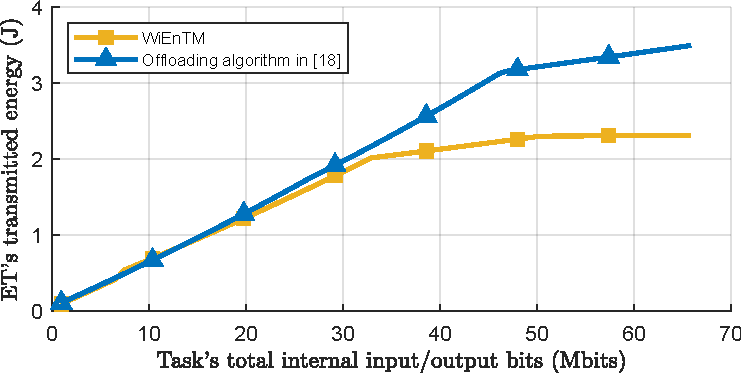
\includegraphics[width=\linewidth]{simulation2_b.pdf}
		\caption{} \label{fig:7brr}
	\end{subfigure}
	
	\caption{\textcolor{blue}{Comparison of ET's transmitted energy between WiEnTM and the algorithm proposed in \cite{b13} for different a) task's CPU cycles (i.e., $\sum_{v_d\in\mathcal{V}_d}C_{v_d}$) and, b) task's internal input/output bits (i.e., $\sum_{v_d^i,v_d^j\in\mathcal{V}_d}N_{v_d^i,v_d^j}$).}} \label{fig:7rr}
\end{figure}

\begin{figure}
	\centering
	\begin{subfigure}[b]{.24\textwidth}
		\centering
		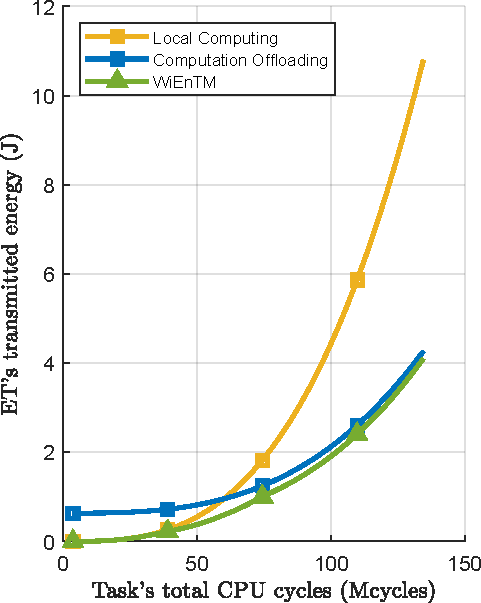
\includegraphics[height=1.2\linewidth]{simulation3_a.pdf}
		\caption{} \label{fig:10a}
	\end{subfigure}
	\begin{subfigure}[b]{.24\textwidth}
		\centering
		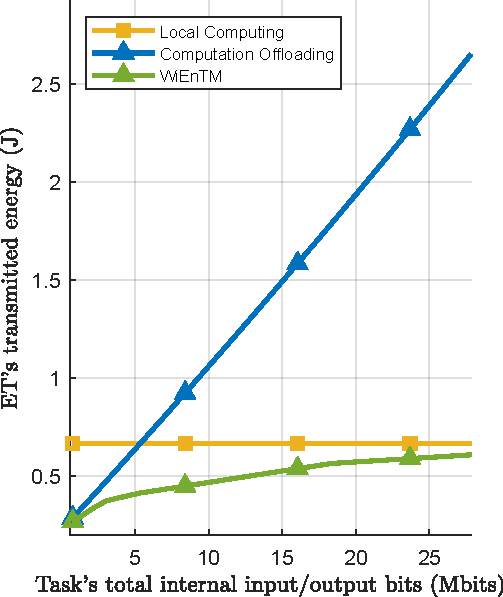
\includegraphics[height=1.2\linewidth]{simulation3_b.pdf}
		\caption{} \label{fig:10b}
	\end{subfigure}
	
	\caption{\textcolor{blue}{Comparison of ET's transmitted energy for three offloading policies when there are 200 WDs. 1) Local computation only, 2) computation offloading only, and 3) WiEnTM algorithm.}} \label{fig:10}
\end{figure}

\begin{my}{1cm}{1cm}
	\rev{
	We further investigate the performance of our proposed WiEnTM algorithm by evaluating the ET's transmitted energy in comparison to that of \cite{b13}. Figs. \ref{fig:7arr} and \ref{fig:7brr} illustrate the effect of the task's CPU cycles and the task size (i.e., the number of input/output bits), respectively. The results show that by using WiEnTM, the ET consumes up to $34\%$ less energy compared to the algorithm in \cite{b13}.
	
	$\cdots$
		
	We now consider 200 WDs and investigate the ET transmission energy required to enable WDs execute their tasks. We study three different policies: 1) Local computing, 3) computation offloading, and 3) WiEnTM algorithm. We assume that among these devices, 100 WDs have a task with the call graph shown in Fig. \ref{fig:5a} and the rest with the task call graph of Fig. \ref{fig:5b}.
		
		$\cdots$
		
	Fig. \ref{fig:10a} shows the ET's energy transmission when we vary the task's total CPU cycles. Additionally, Fig. \ref{fig:10b} illustrates the ET's energy for different numbers of the task's total  input/output bits, which reflect the size of the tasks.
	
		$\cdots$
	
	In particular, according to Fig. \ref{fig:10a}, comparing to the local computing case, a higher improvement is obtained for the computationally intensive tasks.
	
		$\cdots$
		
	The results of Fig. \ref{fig:10b} imply that WiEnTM mainly follows the policy of offloading to edge/cloud server for tasks with a small number of input/output bits. As we increase the number of bits, the algorithm tends to rely more on local computing. As can be observed, WiEnTM greatly outperforms both schemes.
	}\newline
\end{my}

Furthermore, the dependencies between subtasks of each WD are shown in Fig. \ref{fig:5}. We have included the following sentences in Section V of the revised manuscript to further clarify this issue.\newline

\begin{my}{1cm}{1cm}
	\rev{
		These figures show the dependencies in the task call graph of each WD. An arrow leaving node $i$ toward $j$ indicates that subtask $j$ is dependent on subtask $i$.
	}\newline
\end{my}

\end{enumerate}

We would like to gratefully thank the reviewer for the valuable comments and suggestions. We hope that we have addressed these comments satisfactorily.\newline

\section{Response to Reviewer 4}
\begin{enumerate}
	
	
	\item \underline{Reviewer's Comment}: \textit{````an'' MEC rather than ``a'' MEC;''} \newline
	
	\underline{Authors' Reply}: We have applied the reviewer's comment throughout the paper and updated the manuscript.\\
	
	\item \underline{Reviewer's Comment}: \textit{``This paper considers half-duplex transmission for WDs, where computation offloading cannot be performed simultaneously with energy harvesting. How about the full-duplex?''} \newline
	
	\underline{Authors' Reply}: Inspired by \cite{b2,b10,b11,b14}, in our work, we consider half-duplex transmission for WDs. Due to the production costs, battery-less devices usually lack a full-duplex transceiver. In the case that devices are equipped with full-duplex transceivers, we do not need a harvest-then-offload mechanism as both offloading and energy harvesting can be done simultaneously. There are several works studying simultaneous wireless information and power transfer (SWIPT) \cite{b8} for devices with full-duplex transmission. However, this is beyond the scope of our work and is considered for future works. We have added the following explanations to Section II of the revised manuscript. \newline
		
	\begin{my}{1cm}{1cm}
		\rev{
			In contrast, for the case of full-duplex transmission, scheduling algorithms are categorized as the simultaneous wireless information and power transfer (SWIPT) \cite{b8} mode. However, considering the constraints of the production costs and devices' form factor for battery-less WDs, they usually lack a full-duplex transceiver to perform energy harvesting and data transmission simultaneously.
		}\newline
	\end{my}
	
	We have also added the following sentence to Section VI of the revised manuscript.

	\begin{my}{1cm}{1cm}
		\rev{
				We will also study more powerful WDs with full-duplex capability in future.
		}\newline
	\end{my}
	
	
	\item \underline{Reviewer's Comment}: \textit{``The font size in Fig. 2 should be adjusted. For example, the font is too large for ``WET''.''} \newline
	
	\underline{Authors' Reply}: We have adjusted the font size of Fig. \ref{fig2r} as suggested. \newline
	
	\renewcommand{\figurename}{Fig.}
	\renewcommand{\thefigure}{2}
	\begin{my}{1cm}{1cm}
		\rev{
			\begin{figure}[h!]
				\centering
				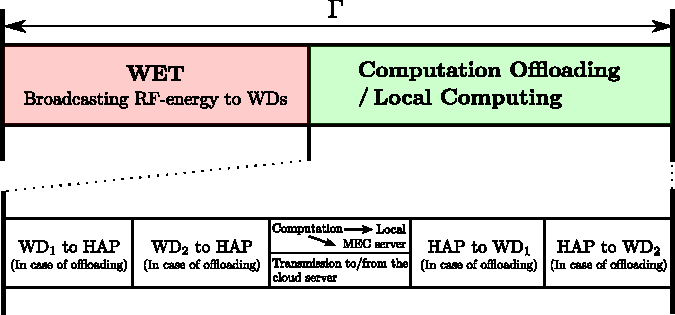
\includegraphics[height=95pt]{TDMA.pdf}
				\caption{\textcolor{blue}{Harvest-then-offload scheduling with TDMA protocol for a system of two WDs. An episode of length $\Gamma$ is divided into two times frames of WET and offloading/local computing. In the case of offloading, the offloading/local computing time frame consists of three slots. The first and last slots are for transmitting the data and retrieving the results, respectively. The second slot is dedicated to the computation in the MEC server or transmission to/from the cloud server.}}\label{fig2r}
			\end{figure}
		}
	\end{my}
	
	\item \underline{Reviewer's Comment}: \textit{``The authors state that “the partial offloading provides a more realistic model of tasks”. It is suggested to provide more explanation.''}\newline
	
	\underline{Authors' Reply}: In the partial offloading model, each task is represented by its call stack which exactly maps to a real computer program. Note that binary offloading is a special case of partial offloading when we only consider a single partition. To further clarify this issue, we have included the following explanation in Section II of the revised manuscript.\newline
	
	\begin{my}{1cm}{1cm}
		\rev{
			The partial offloading provides a more realistic model of tasks as it leverages the task call graph to represent each task. This accurately models the call stack of a computer program.\newline
		}
	\end{my}

	We have also provided an application example in the footnote of Page 3 as below.\newline
	
	\begin{my}{1cm}{1cm}
		\rev{
			\textcolor{blue}{For instance, \textit{Pyan}\cite{b41} is a Python module that generates the task call graph of a Python code by analysis of its modules and functions.}\newline
		}
	\end{my}

	\item \underline{Reviewer's Comment}: \textit{``Why ``the cumulative energy consumption of the devices is no more than their harvested energy''? could you please give a realistic example to illustrate the assumption?''}\newline
	
	\underline{Authors' Reply}: Indeed, the cumulative energy consumption of devices must be no more than their harvested energy. It is because we consider wireless-powered devices which cannot store energy for later use. Thus, the devices cannot use more energy than the harvested amount. It also ensures the sustainable operation of the devices. The same assumption has been made in similar works \cite{b10,b30,b13,b39,b26,b2}. We have included the following sentences in Section II of the revised manuscript to make this fact more clear.\newline
	
	\begin{my}{1cm}{1cm}
		\rev{
			As described earlier, we assume sustainable operation of WDs by only relying on the harvested energy (i.e., battery-less network). Thus, the cumulative energy consumption of the devices on each episode must be no more than their harvested energy.\\
		}
	\end{my}

	\item \underline{Reviewer's Comment}: \textit{``More recent and important references are required.''}\newline
	
	\underline{Authors' Reply}: To address the reviewer's comment, we have removed a few of outdated references and cited five recently published papers as follows. \newline
	\begin{my}{1cm}{1cm}
		\rev{
	{\small
		\noindent\cite{b35} Y. Yu, Y. Yan, S. Li, and D. Wu, ``Task delay minimization in wireless powered mobile edge computing networks: A deep reinforcement learning approach,'' in \textit{Proc. of Int. Conf. Wireless Commun. Signal Process. (WCSP)}, Changsha, China, Mar. 2021.\\[10pt]
		\cite{b38} Y. Li, Y. Wu, M. Dai, B. Lin, W. Jia, and X. Shen, ``Hybrid NOMA-FDMA assisted dual computation offloading: A latency minimization approach,'' \textit{IEEE Trans. Netw. Sci. Eng.}, vol. 9, no. 5, pp. 3345--3360, Sep. 2022.\\[10pt]
		\cite{b37} K. Guo, M. Yang, Y. Zhang, and J. Cao, ``Joint computation offloading and bandwidth assignment in cloud-assisted edge computing,'' \textit{IEEE Trans. Cloud Comput.}, vol. 10, no. 1, pp. 451--460, Mar. 2022.\\[10pt]
		\cite{b39} R. Zhang and C. Zhou, ``A computation task offloading scheme based on mobile-cloud and edge computing for WBANs,'' in \textit{Proc. of IEEE Int. Conf.	Commun. (ICC)}, Seoul, Korea, Repulic of, Mar. 2022.\\[10pt]
		\cite{b40} Z. Gao, W. Hao, and S. Yang, ``Joint offloading and resource allocation for multi-user multi-edge collaborative computing system,'' \textit{IEEE Trans. Veh. Technol.}, vol. 71, no. 3, pp. 3383--3388, Mar. 2022.}\\}
	\end{my}

	We have also cited these works in the following sentences in Section I of the revised manuscript.\\
	
	\begin{my}{1cm}{1cm}
		\rev{
			Mobile edge computing (MEC) is a state-of-the-art computation paradigm to address the challenge of insufficient computing resources in Internet of Things (IoT) networks \cite{b35, b4}. By deploying the edge servers, nearby devices can offload their computation tasks. Dispatching those tasks that require a higher amount of energy will let devices save more energy \cite{b38}. However, as the computation tasks become more and more intensive, a coordination with cloud servers might be inevitable \cite{b37}. As a result, three-tier models consisting of cloud, edge, and IoT devices are introduced to overcome the aforementioned challenges \cite{b5,b6,b39,b40}.
			
			$\cdots$
			
			In the existing work \cite{b39}, authors proposed a scheme that aims to minimize the total cost in terms of energy and delay for a three-tier cloud-edge-IoT system. Gao \textit{et al.} in \cite{b40} proposed an offloading algorithm to minimize an objective called the energy time cost (ETC) for a three-tier network. Although \cite{b5}, \cite{b39}, and \cite{b40} all benefit from a computationally-scalable three-tier system, IoT devices still rely on battery energy and they thus lack the sustainability feature of WPMEC systems.
			\\}
	\end{my}
	
\end{enumerate}

We would like to gratefully thank the reviewer for the valuable comments and suggestions. We hope that we have satisfactorily addressed these comments.\newline

\end{document}


